\chapter{Delay and Predict Dereverberation Parameters}

\section{Multi-channel Linear Prediction Order}

\textbf{MINT Results}

\begin{figure}[H]
	\centering
	%
	\begin{subfigure}[c]{0.2\textwidth}
		\centering
		\begin{minipage}[c][0.3\textwidth][c]{\linewidth} % Height + center alignment
			\centering
			(a) \newline $p2 = L / (M-1)$
		\end{minipage}
	\end{subfigure}
	\begin{subfigure}[b]{0.3\textwidth}
		\centering
		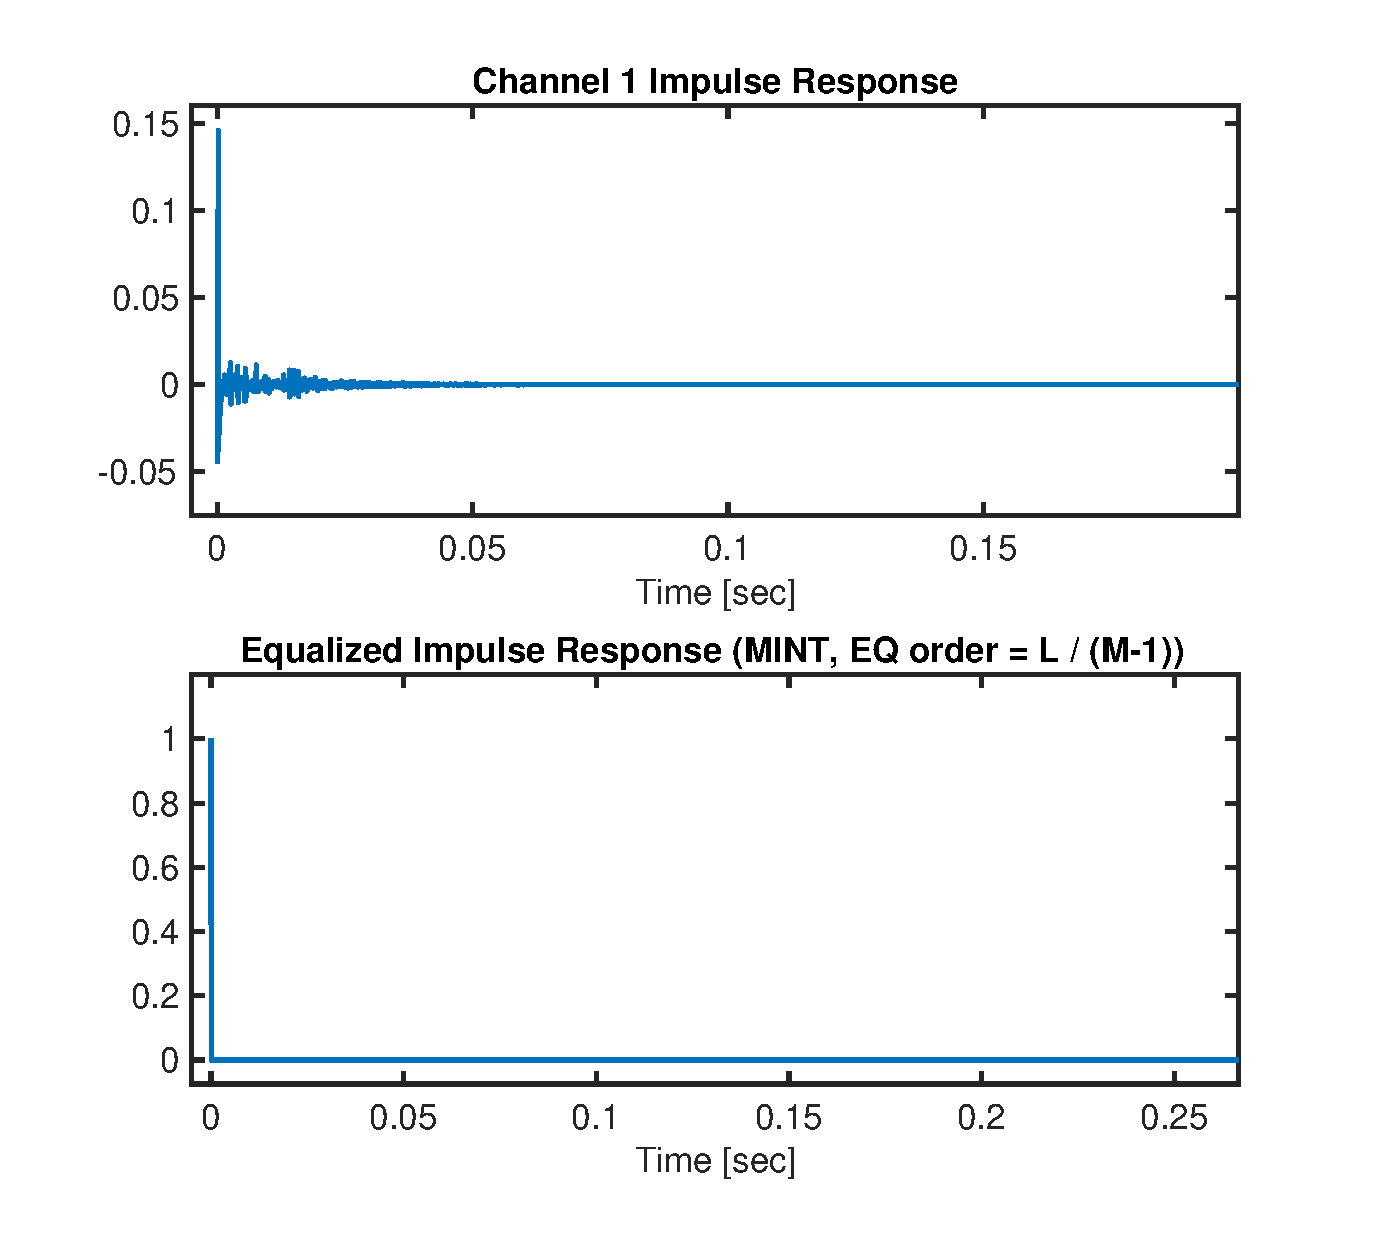
\includegraphics[width=\textwidth]{MINT_EIR_L_div_M_minus_1}
	\end{subfigure}
	\begin{subfigure}[b]{0.3\textwidth}
		\centering
		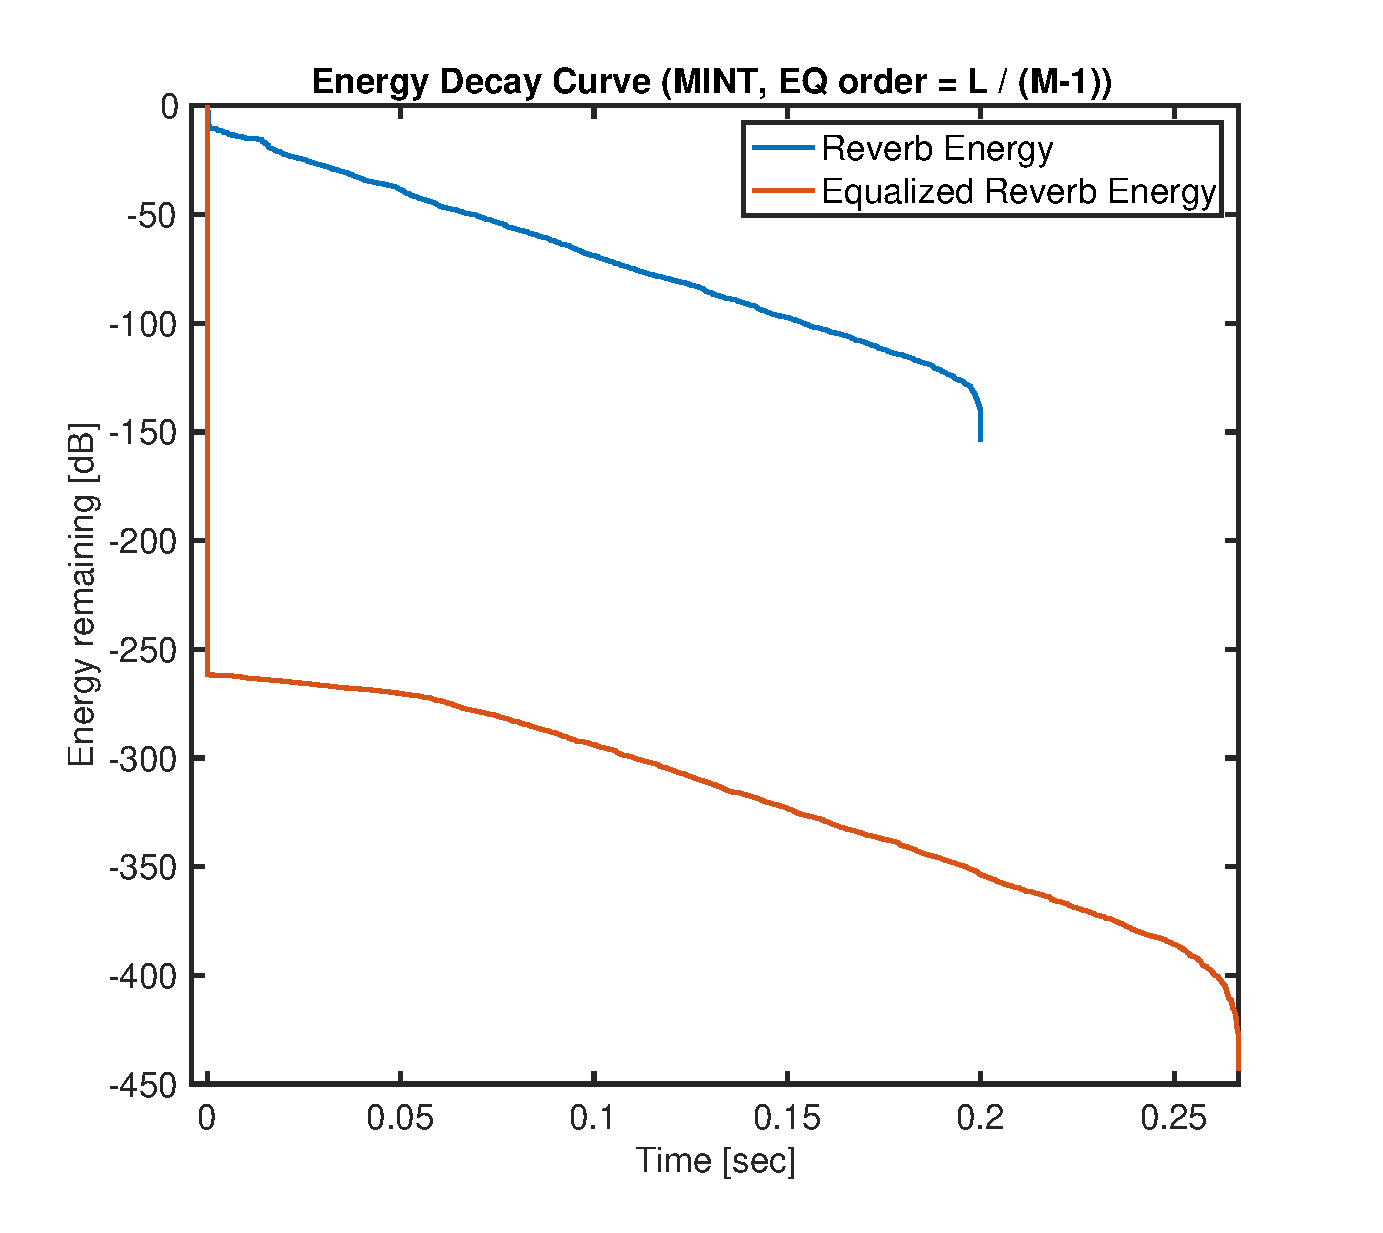
\includegraphics[width=\textwidth]{MINT_EDC_L_div_M_minus_1}
	\end{subfigure}
	%
	\begin{subfigure}[c]{0.2\textwidth}
		\centering
		\begin{minipage}[c][0.3\textwidth][c]{\linewidth} % Height + center alignment
			\centering
			(b) \newline $p2 = N60 / (M-1)$
		\end{minipage}
	\end{subfigure}
	\begin{subfigure}[b]{0.3\textwidth}
		\centering
		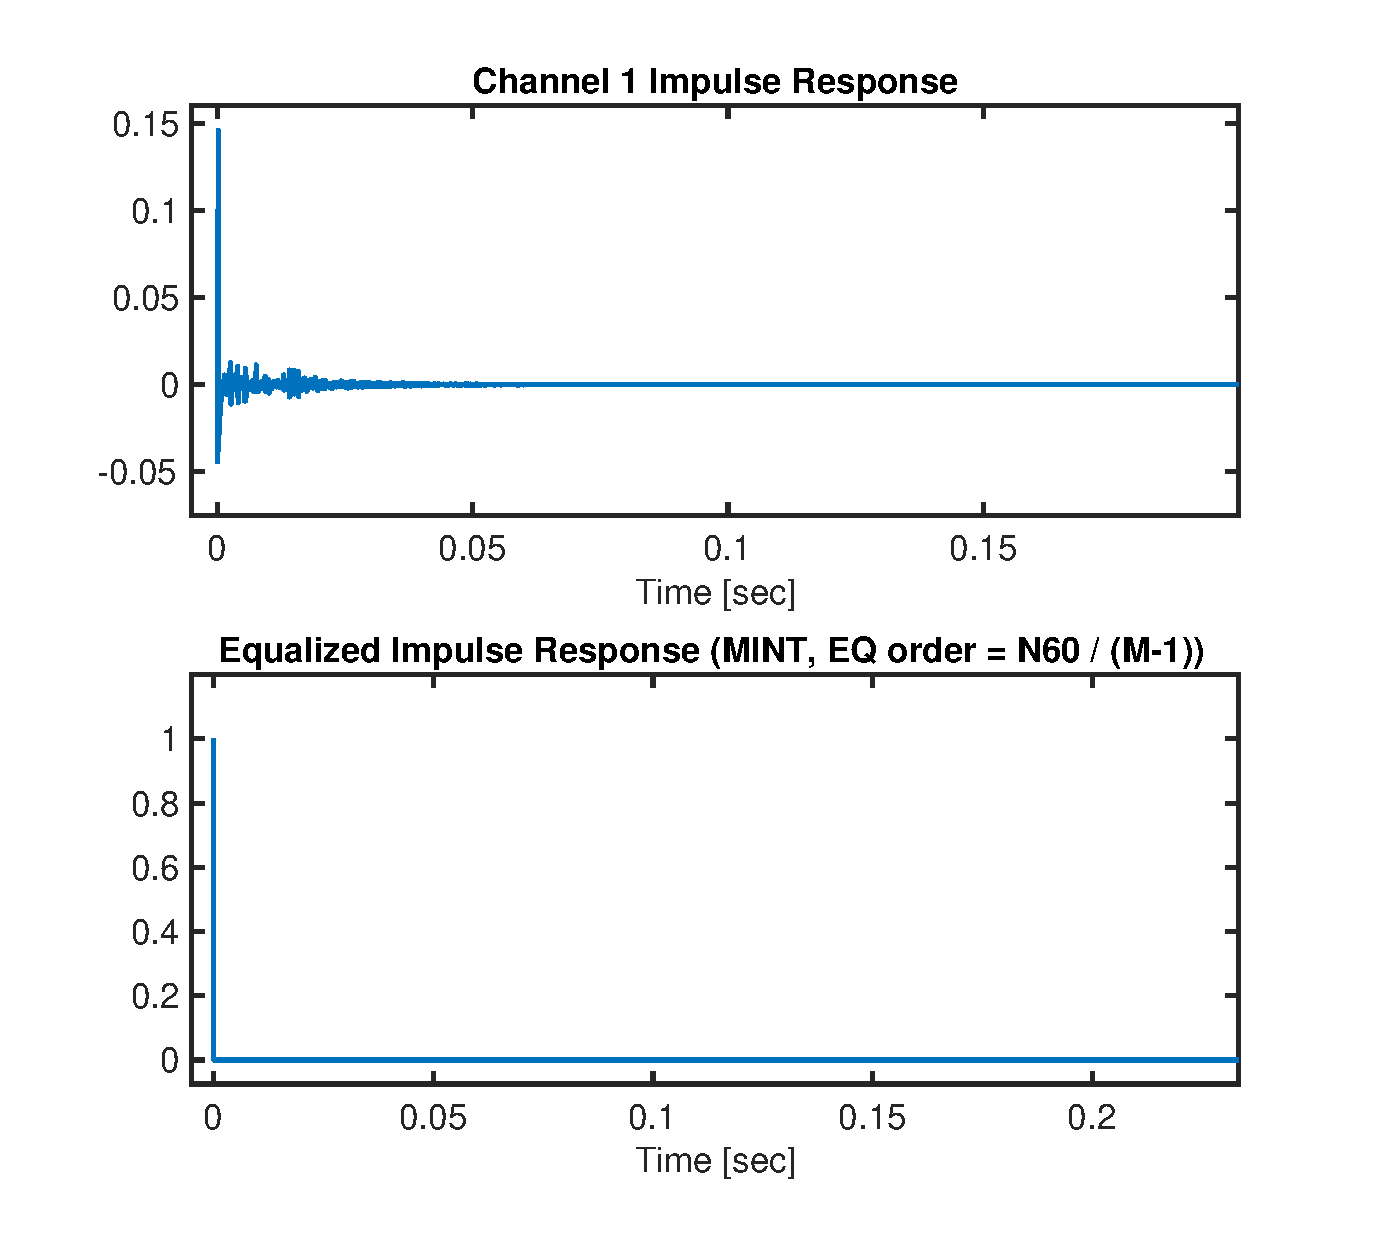
\includegraphics[width=\textwidth]{MINT_EIR_N60_div_M_minus_1}
	\end{subfigure}
	\begin{subfigure}[b]{0.3\textwidth}
		\centering
		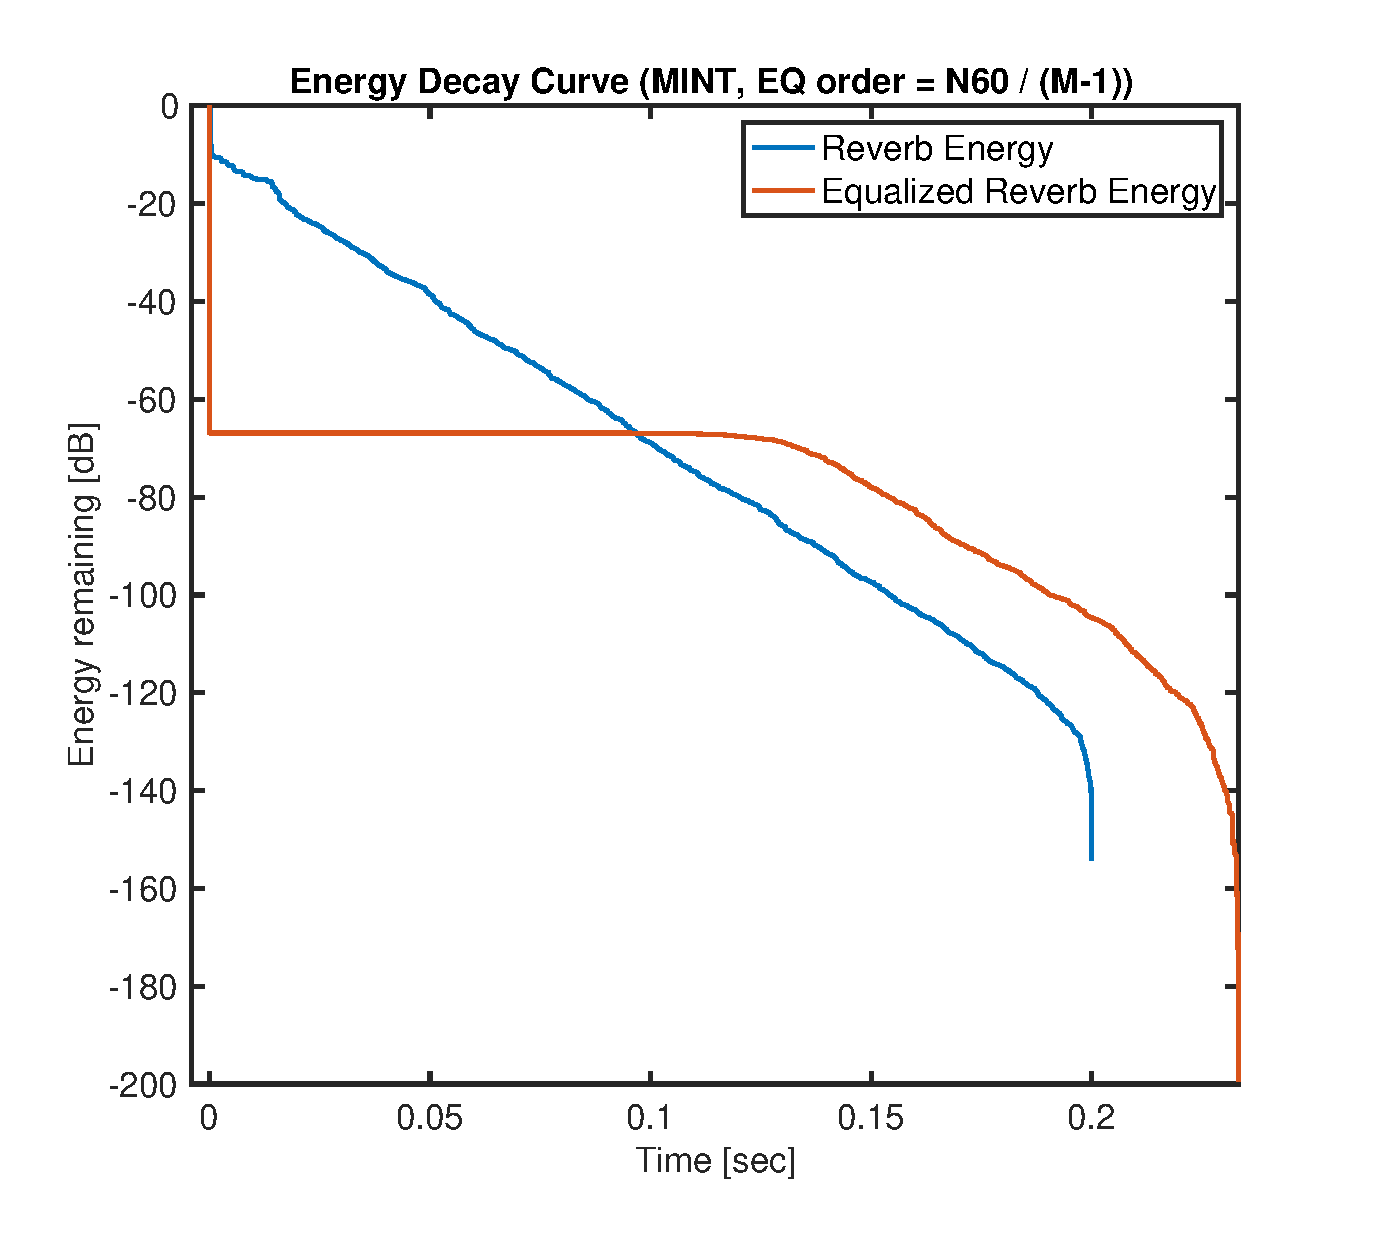
\includegraphics[width=\textwidth]{MINT_EDC_N60_div_M_minus_1}
	\end{subfigure}
	%
	\begin{subfigure}[c]{0.2\textwidth}
		\centering
		\begin{minipage}[c][0.3\textwidth][c]{\linewidth} % Height + center alignment
			\centering
			(c) \newline $p2 = 0.75 \cdot N60 / (M-1)$
		\end{minipage}
	\end{subfigure}
	\begin{subfigure}[b]{0.3\textwidth}
		\centering
		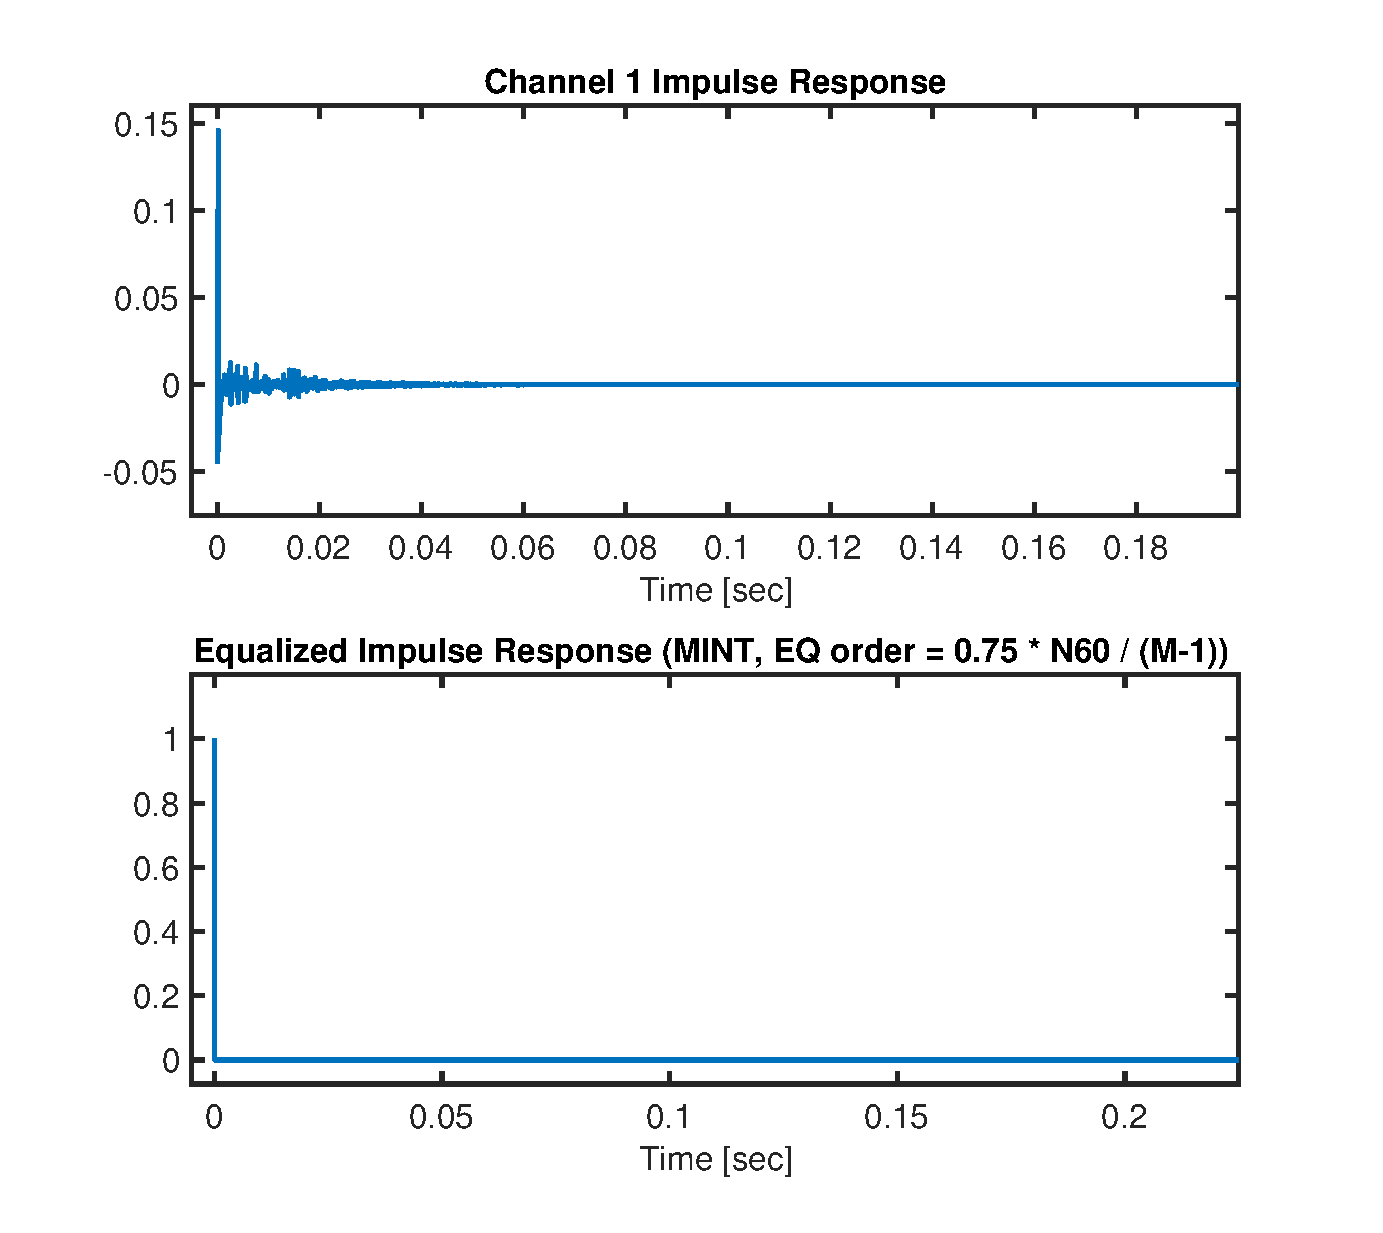
\includegraphics[width=\textwidth]{MINT_EIR_0p75N60_div_M_minus_1}
	\end{subfigure}
	\begin{subfigure}[b]{0.3\textwidth}
		\centering
		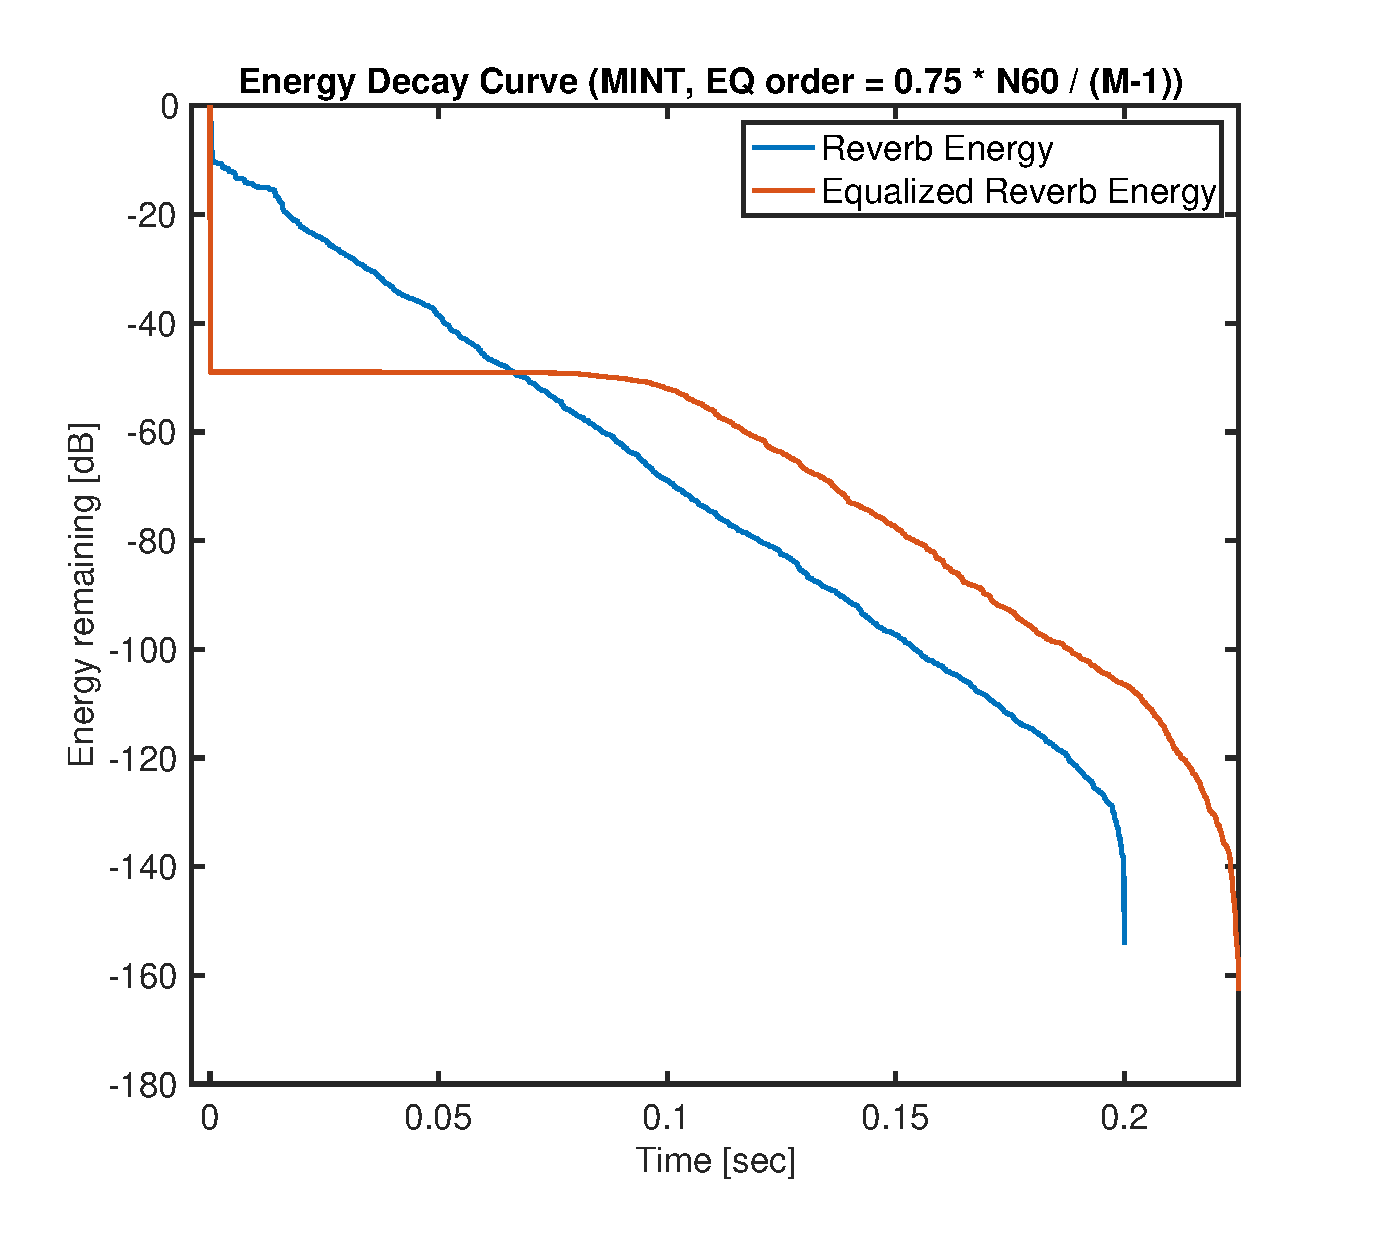
\includegraphics[width=\textwidth]{MINT_EDC_0p75N60_div_M_minus_1}
	\end{subfigure}
	%
	\begin{subfigure}[c]{0.2\textwidth}
		\centering
		\begin{minipage}[c][0.3\textwidth][c]{\linewidth} % Height + center alignment
			\centering
			(d) \newline $p2 = 0.5 \cdot N60 / (M-1)$
		\end{minipage}
	\end{subfigure}
   \begin{subfigure}[b]{0.3\textwidth}
		\centering
		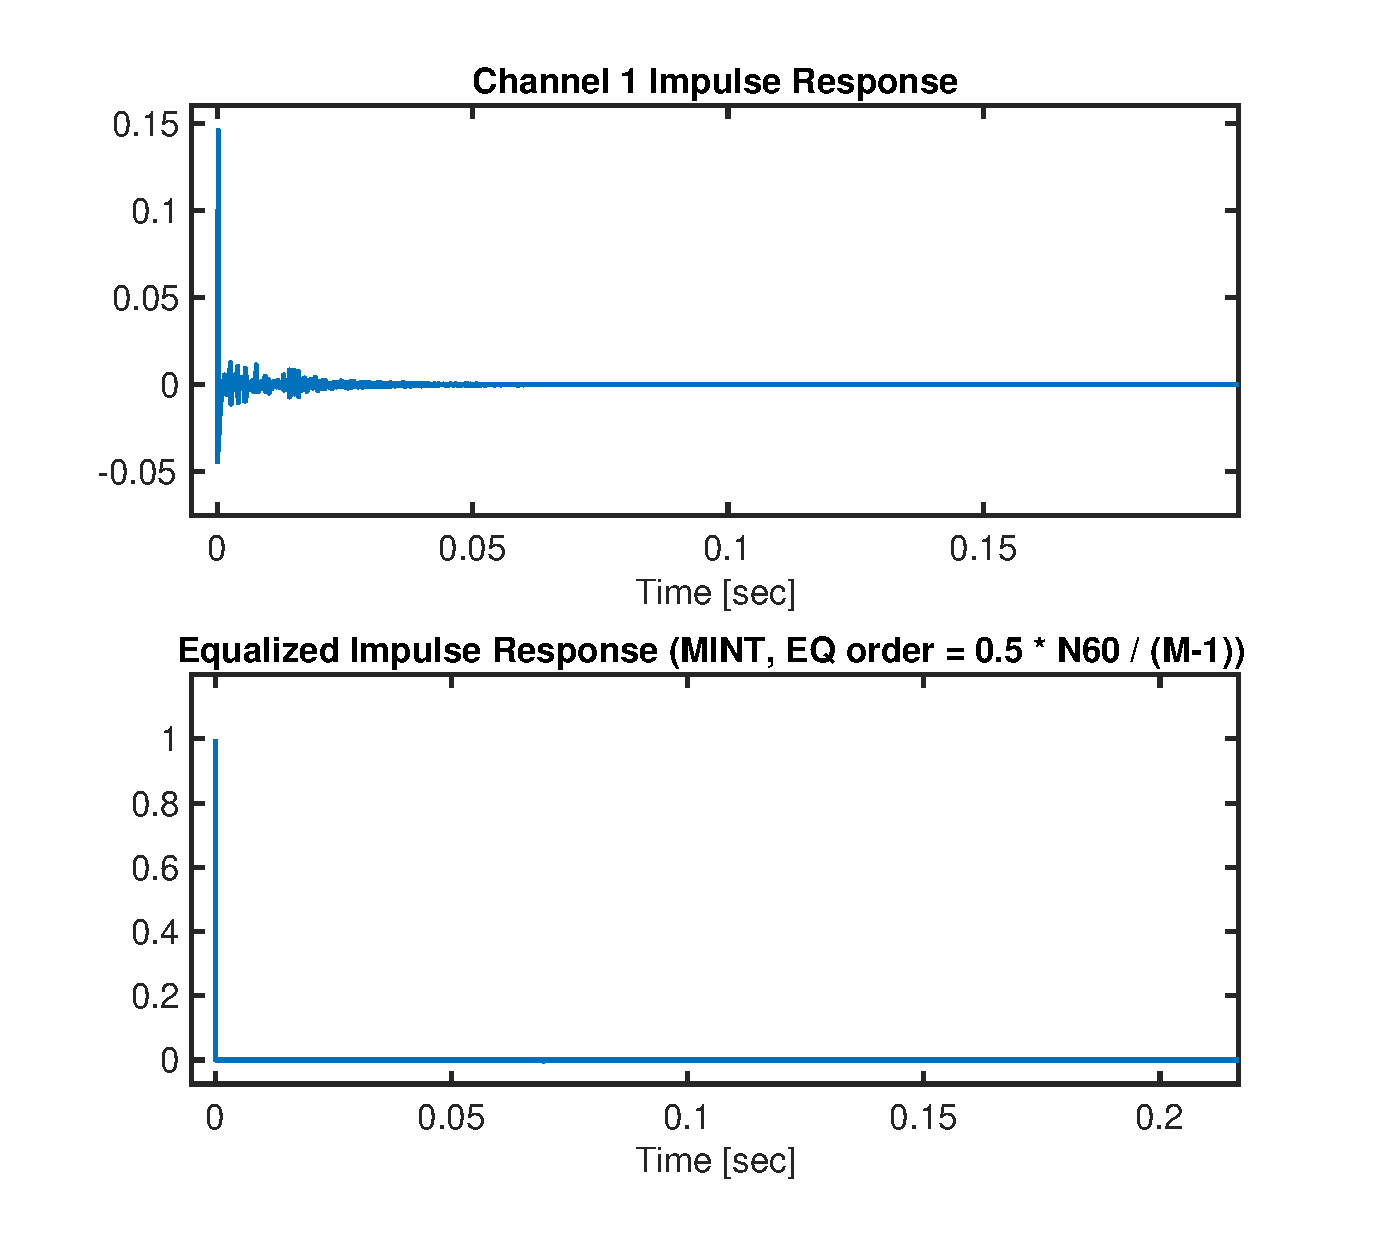
\includegraphics[width=\textwidth]{MINT_EIR_0p5N60_div_M_minus_1}
	\end{subfigure}
	\begin{subfigure}[b]{0.3\textwidth}
		\centering
		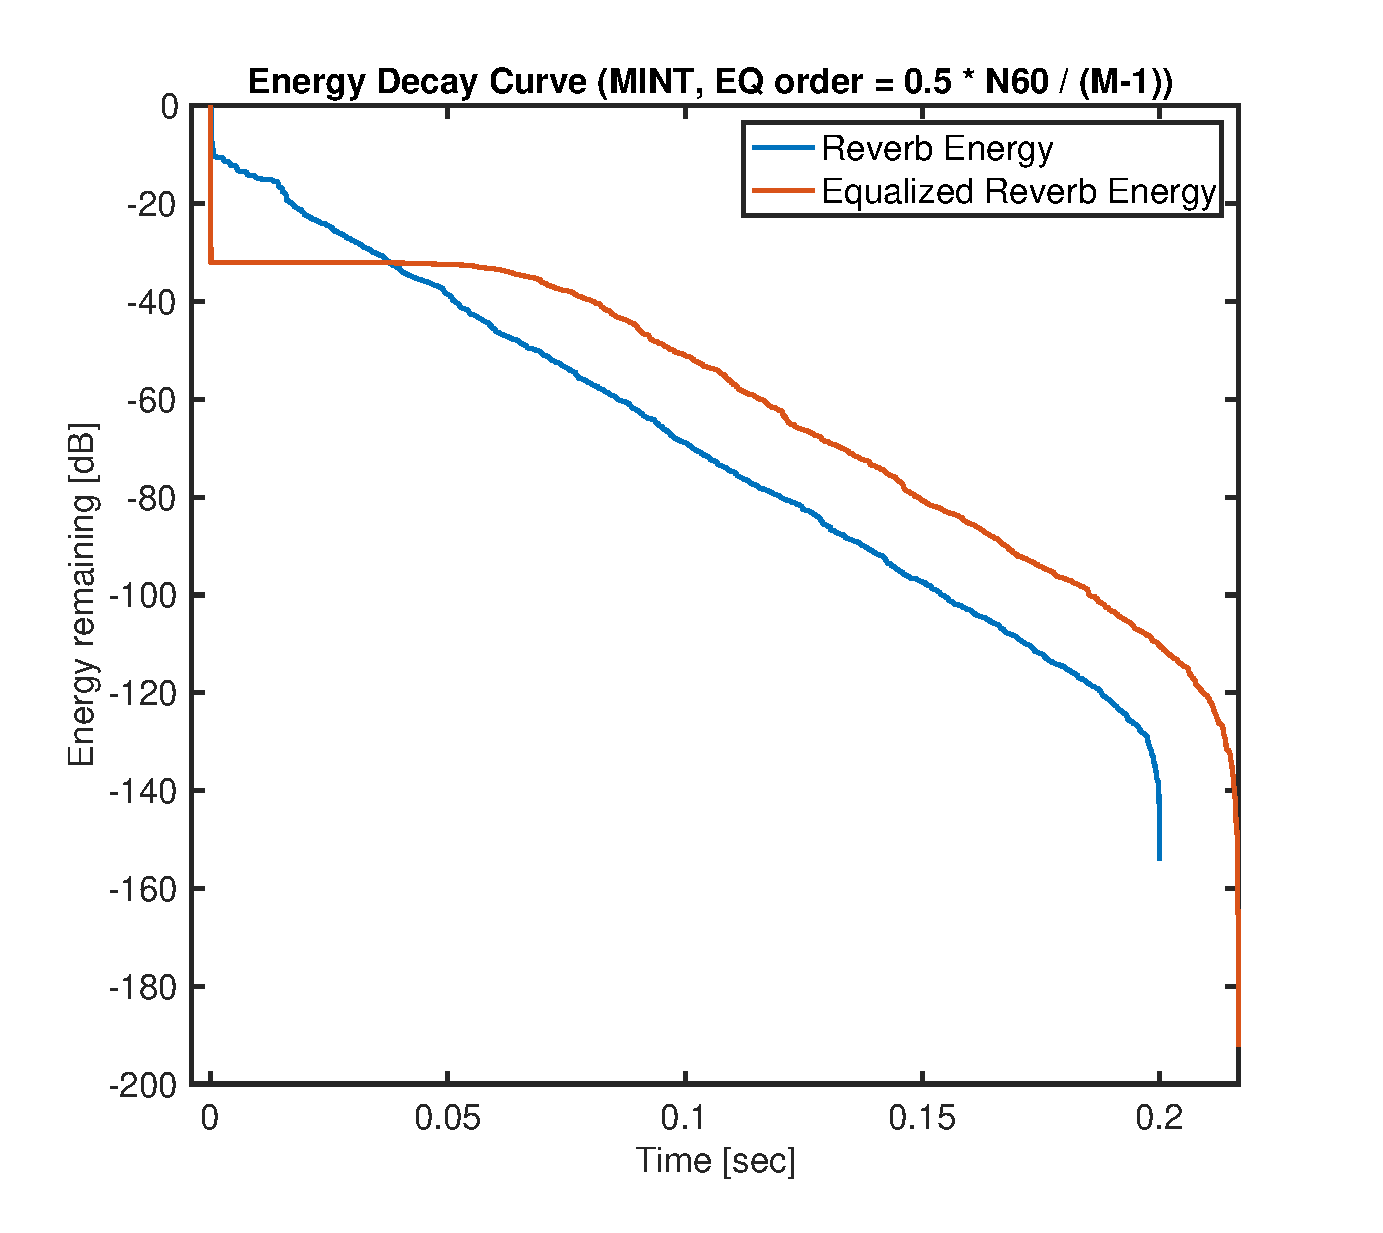
\includegraphics[width=\textwidth]{MINT_EDC_0p5N60_div_M_minus_1}
	\end{subfigure}
	\caption{MINT equalizer performance for various equalizer orders relative to the actual length of the FIR channel ($L$) and the number of samples corresponding to the T60 of the channel ($\mathrm{N60} = \mathrm{T60}  \cdot \mathrm{sample\ rate}$)}
	\label{fig:params_p2_MINT_compare}
\end{figure}

Test Conditions for all:
- Source Signal = SA1.WAV
- Source length = 348366
- RIR = MYRiAD SAL Measured RIR (T60 = 2100 msec, Truncated Exponentially to T60 = 100 msec)
- RIR length = 3200
- T60 = 100 msec (N60 = 1600 samples)
- SNR = 300 dB
- Noise Signal = office ventilation
- SIR = Inf dB
- Interference Signal = None

Delay-and-Predict config:
- Number of Microphones (M) = 4
- Source whitening order (p1) = 4000
- Multichannel Linear Prediction order (p2) = varied
- Source whitening Enabled? = 1
- Source whitening on clean speech? = 1

\textbf{Source Whitening stage, the same in all tests (p1 = 4000)}

\begin{figure}[H]
	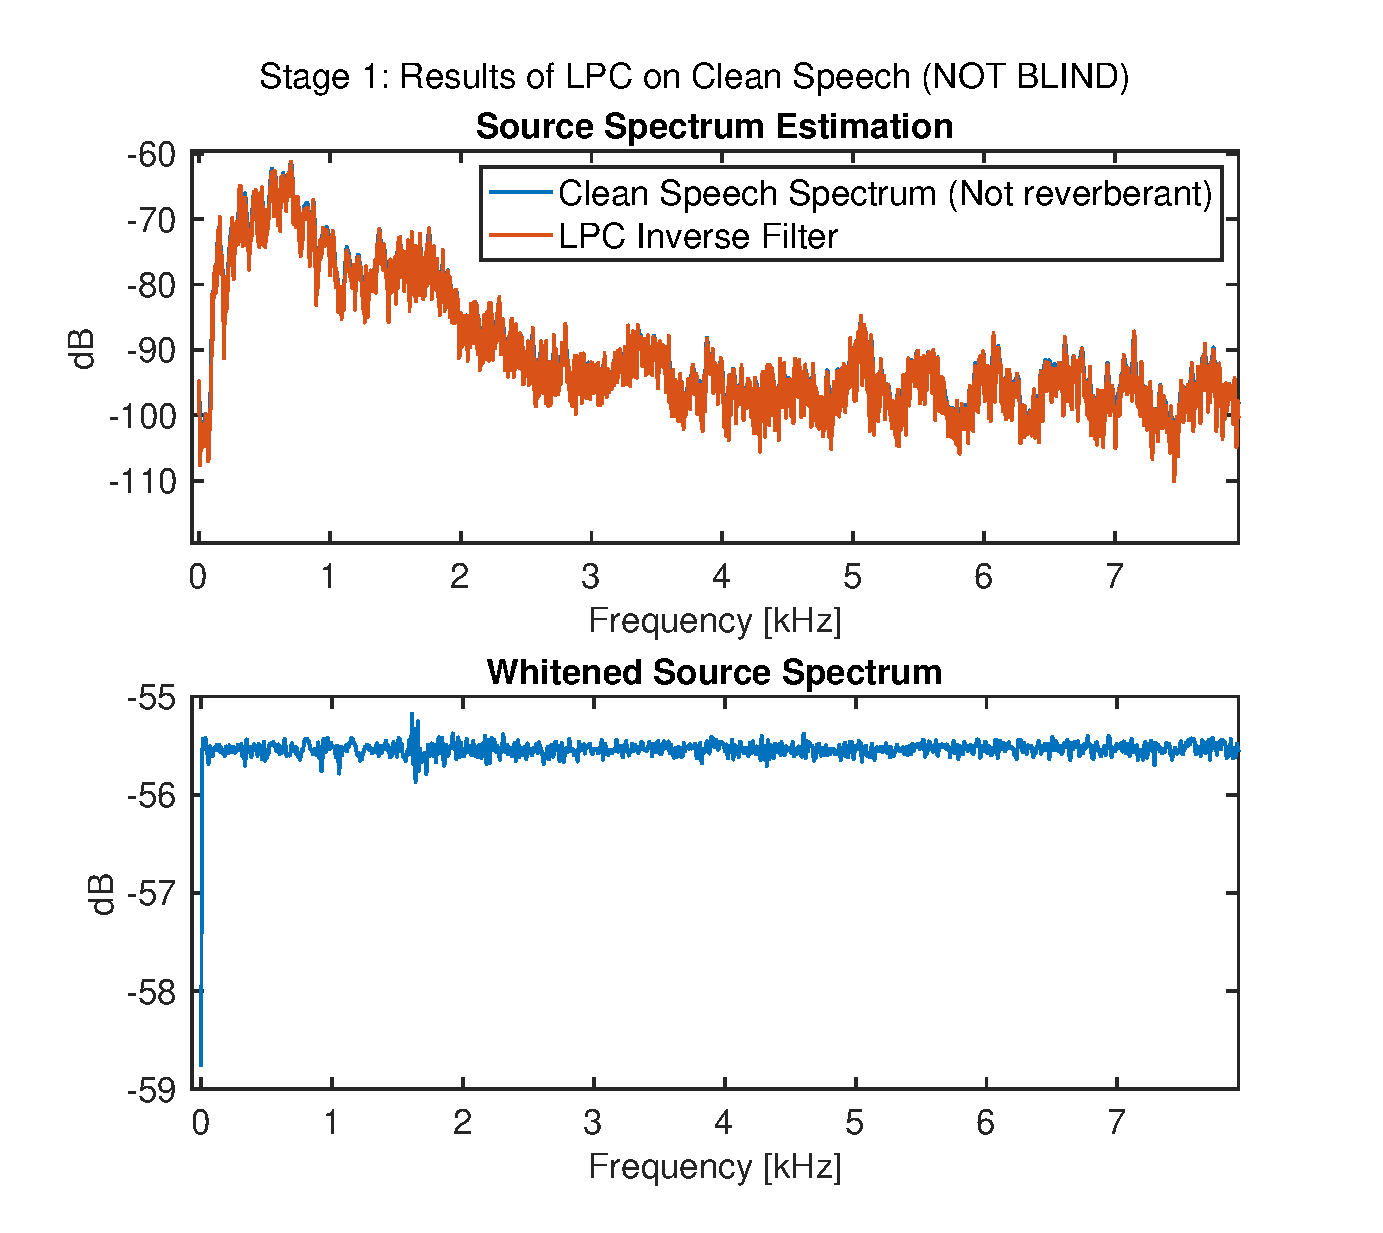
\includegraphics[width=0.49\textwidth]{S1_N60_div_M_minus_1}
	\centering
	\caption{Source whitening results using a $\mathrm{p1} = 4000$ order linear predictor. The prediction error filter coefficients were computed based on clean speech and the same filter was used in all tests in this section to assess the multichannel prediction stage of the delay-and-predict algorithm in isolation.}
	\label{fig:params_p2_stage1}
\end{figure}

\textbf{p2 = L / (M-1) (MINT Condition)}

\begin{figure}[H]
	\centering
	\begin{subfigure}[b]{0.32\textwidth}
		\centering
		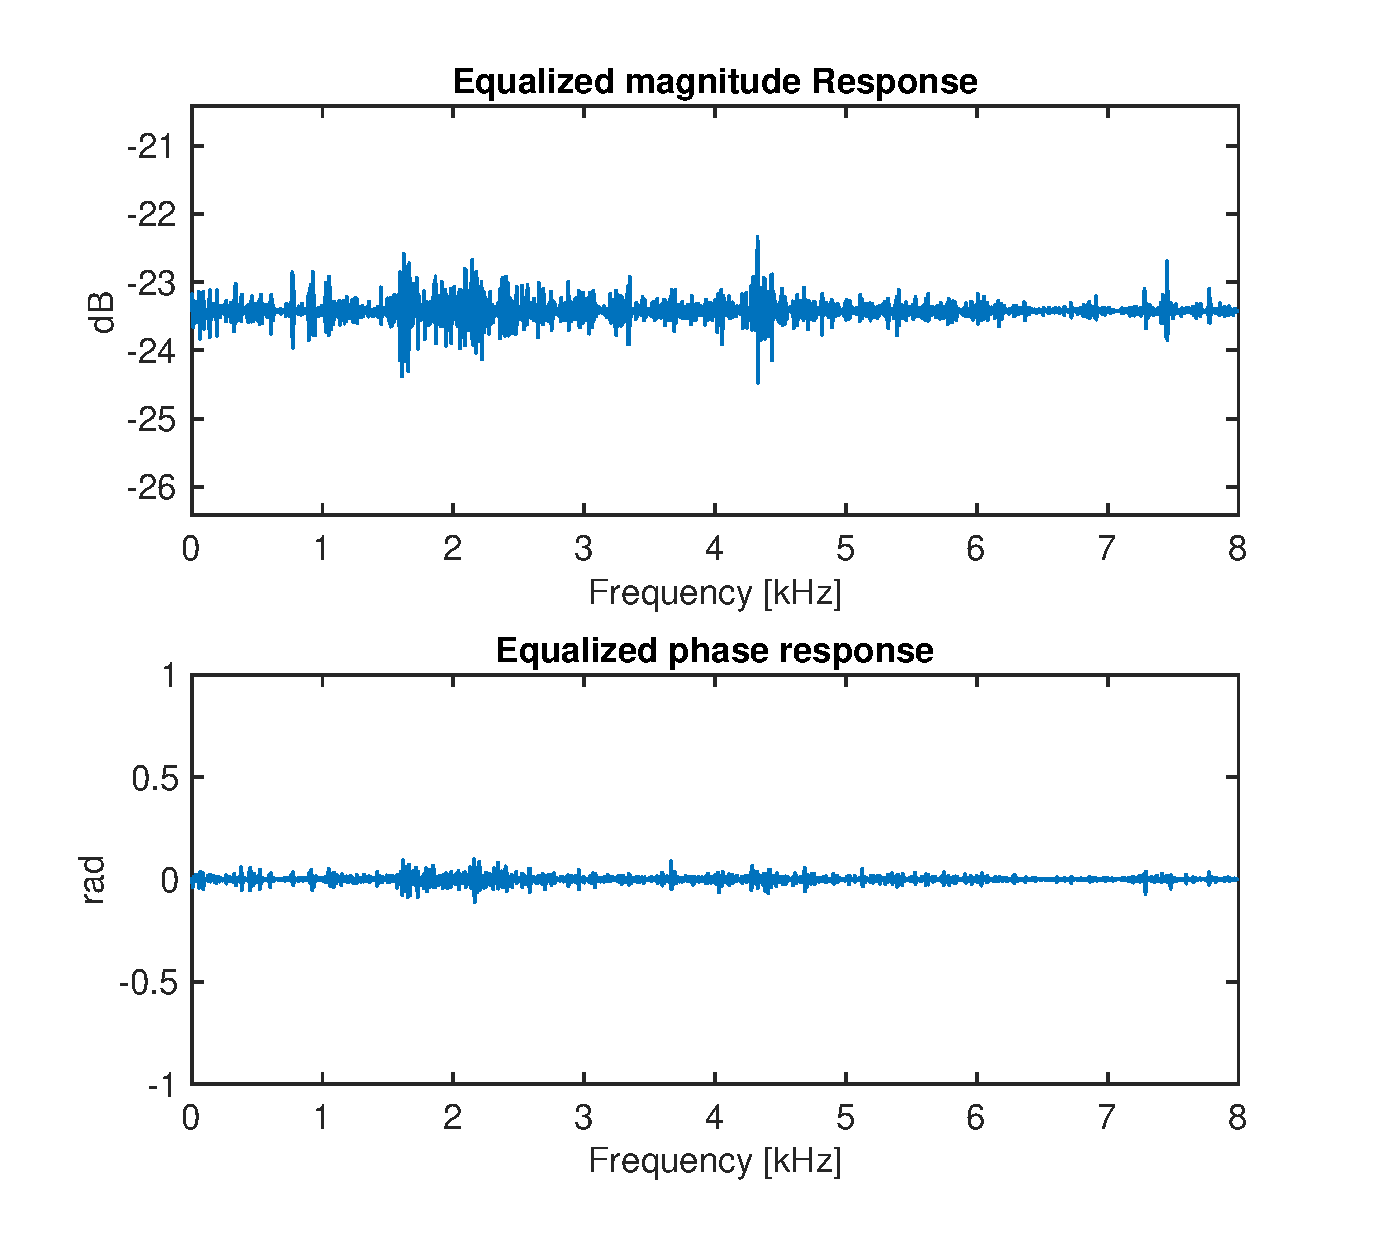
\includegraphics[width=\textwidth]{Equalized_RTF_L_div_M_minus_1}
	    \subcaption{test} \label{subfig:test_subfig_1}
	\end{subfigure}
	\hfill
	\begin{subfigure}[b]{0.32\textwidth}
		\centering
		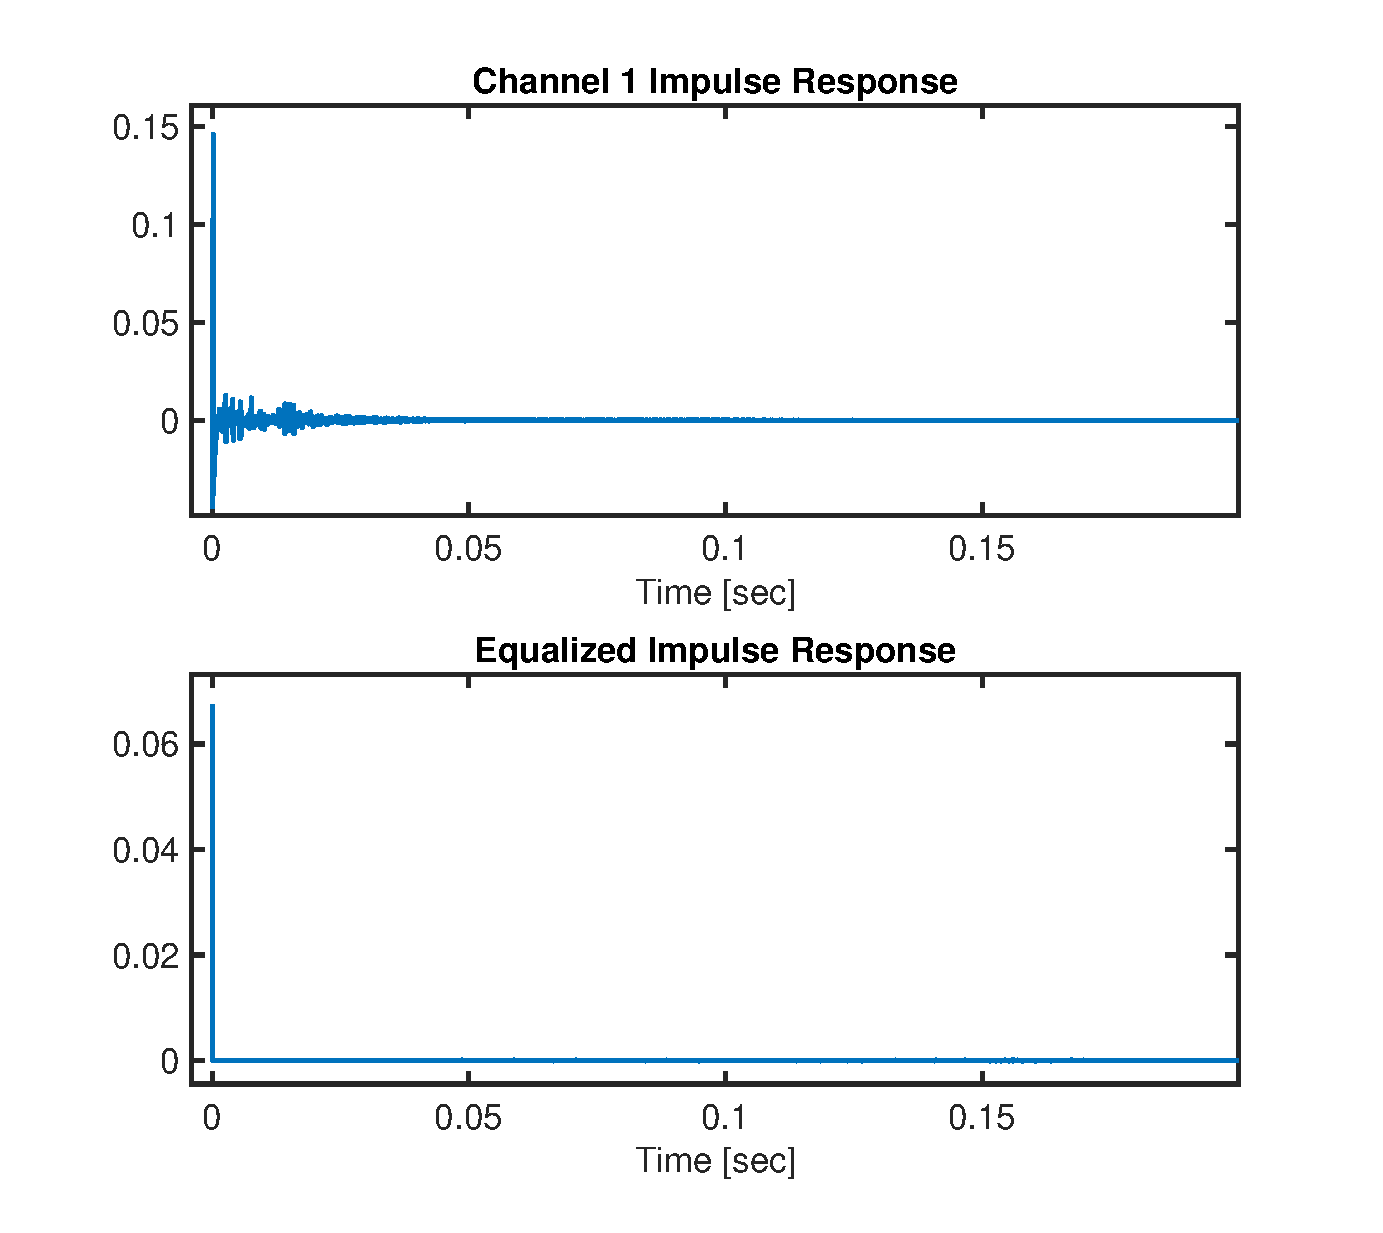
\includegraphics[width=\textwidth]{EIR_L_div_M_minus_1}
	\end{subfigure}
	\hfill
	\begin{subfigure}[b]{0.32\textwidth}
		\centering
		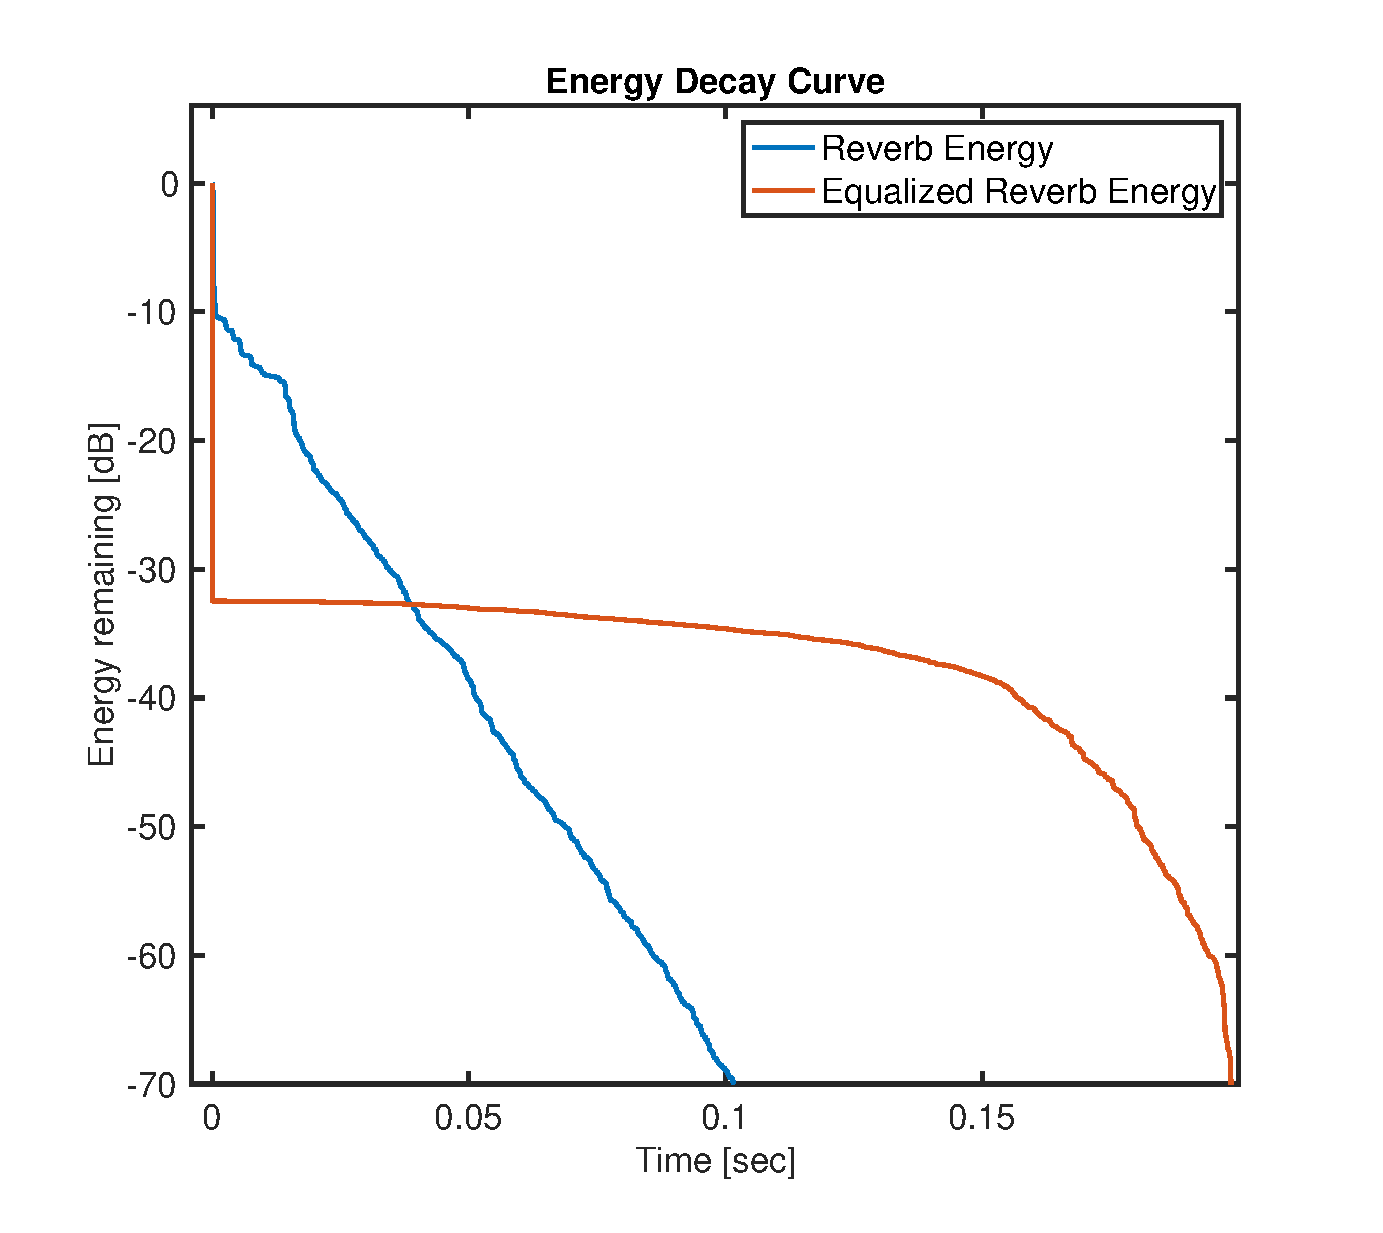
\includegraphics[width=\textwidth]{EDC_L_div_M_minus_1}
	\end{subfigure}
	\hfill
	\caption{Delay-and-Predict dereverberation performance with multichannel linear prediction order $\mathrm{p2} = L / (M-1)$, where $L$ is the FIR RIR length and $M$ is the number of channels. Figure \ref{fig:params_p2_stage1} shows the common source whitening filter used.}
	\label{fig:params_p2_L}
\end{figure}

My subcaption is \ref{subfig:test_subfig_1}.

\textbf{Comparison: p2 = [L  N60  0.75*N60  0.5*N60] / (M-1)}

\begin{figure}[H]
	\centering
	\begin{subfigure}[b]{0.4\textwidth}
		\centering
		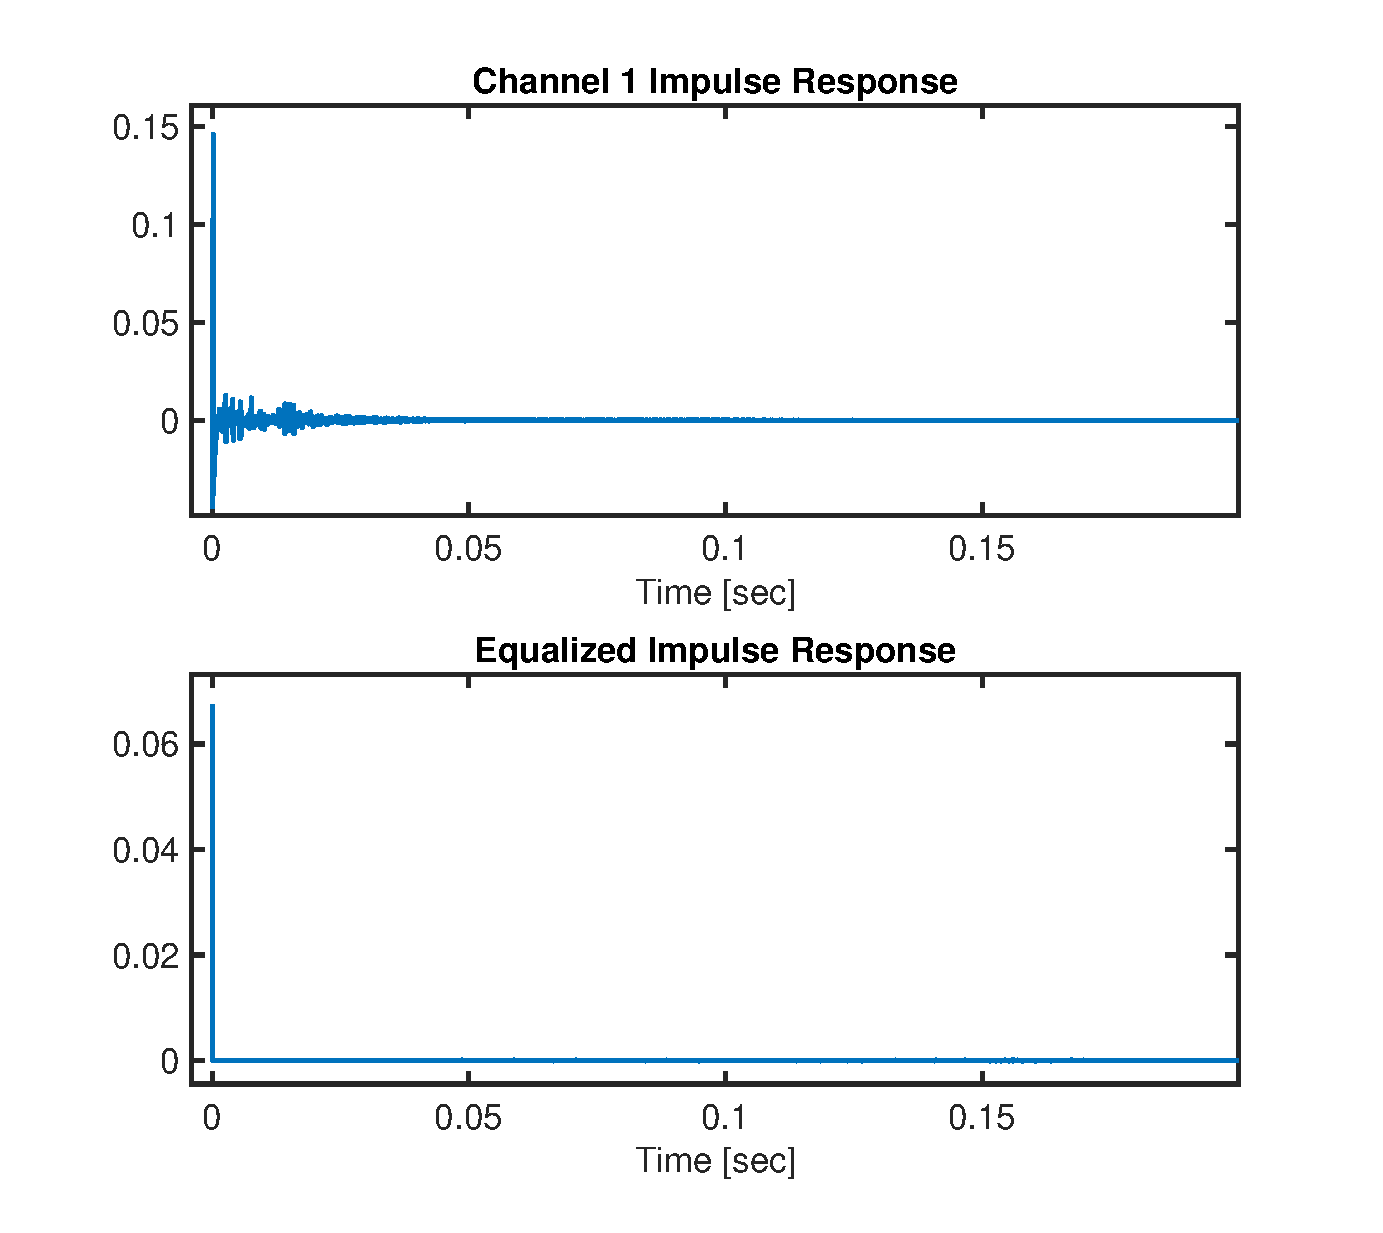
\includegraphics[width=\textwidth]{EIR_L_div_M_minus_1}
	\end{subfigure}
	\begin{subfigure}[b]{0.4\textwidth}
		\centering
		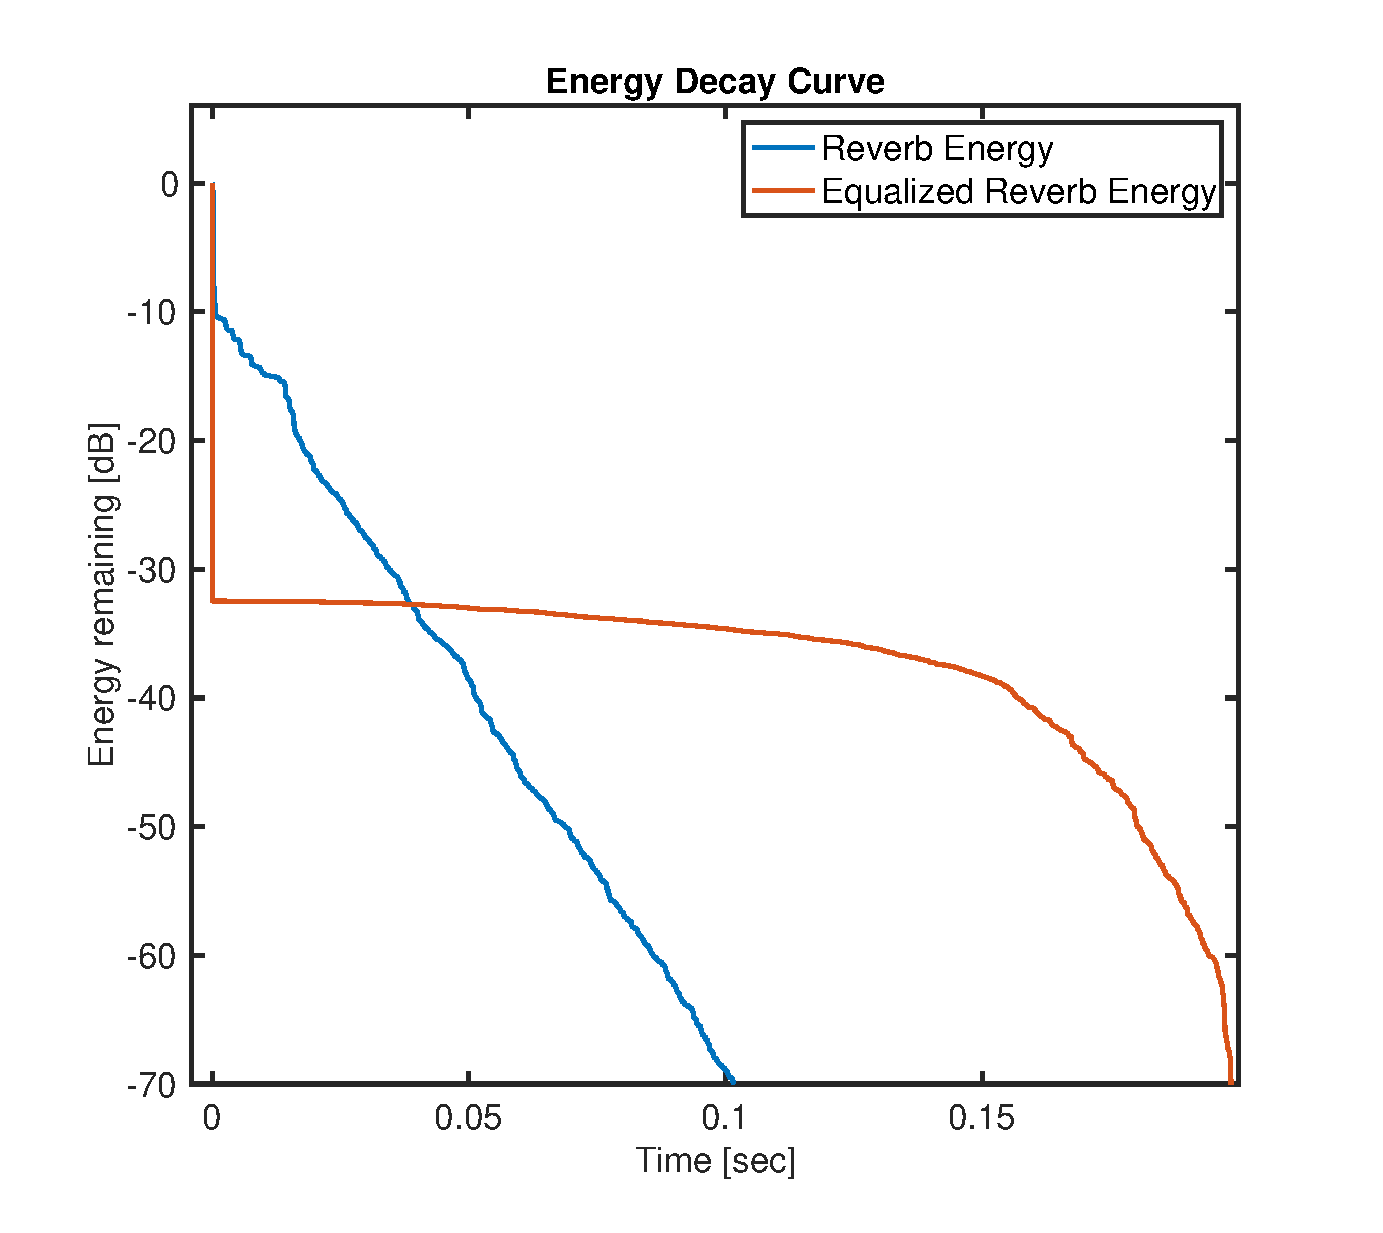
\includegraphics[width=\textwidth]{EDC_L_div_M_minus_1}
	\end{subfigure}
	\begin{subfigure}[b]{0.4\textwidth}
		\centering
		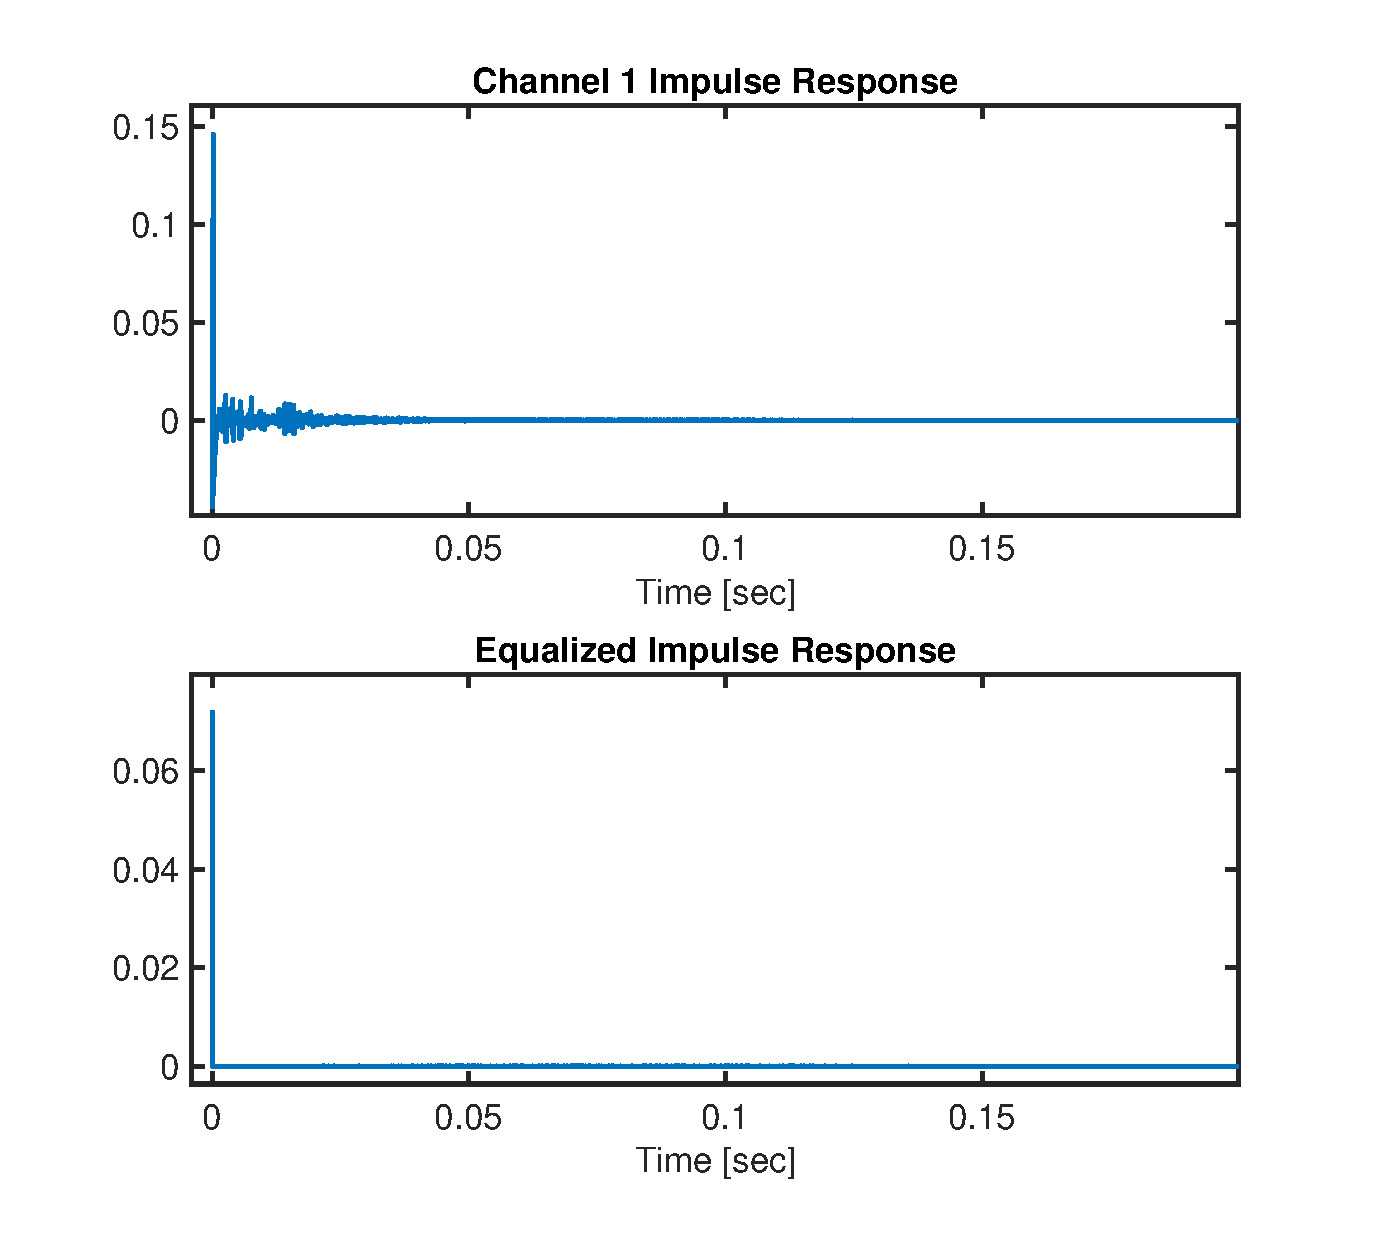
\includegraphics[width=\textwidth]{EIR_N60_div_M_minus_1}
	\end{subfigure}
	\begin{subfigure}[b]{0.4\textwidth}
		\centering
		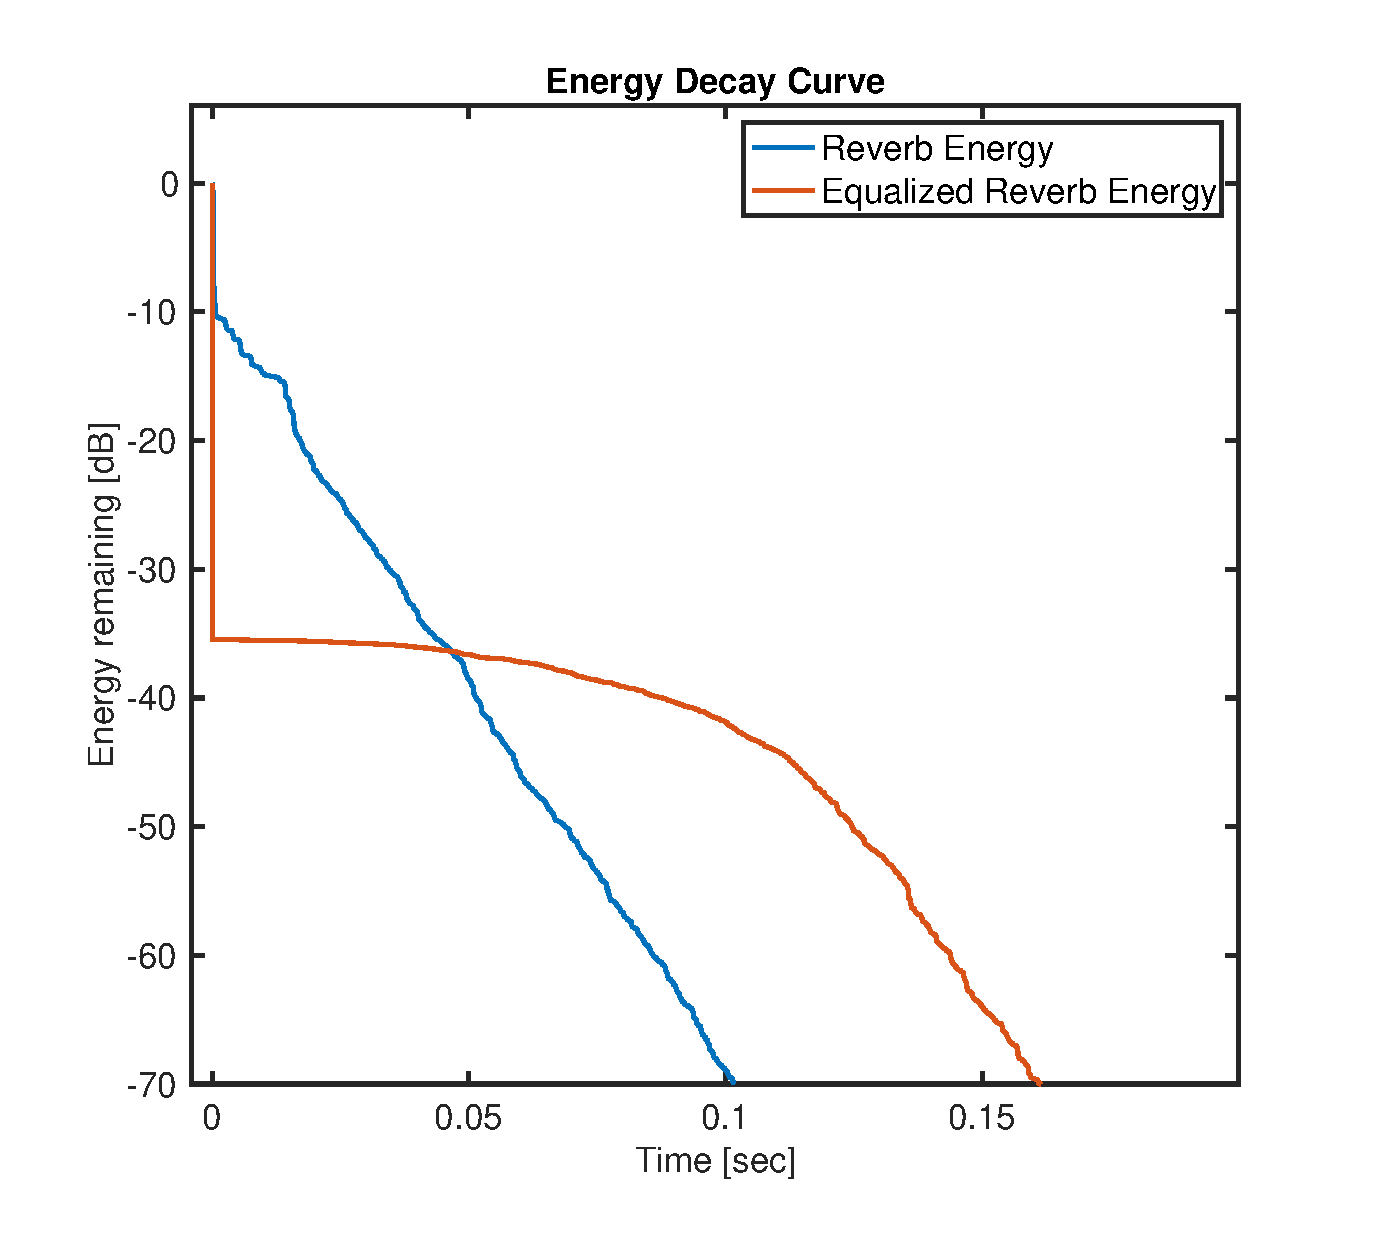
\includegraphics[width=\textwidth]{EDC_N60_div_M_minus_1}
	\end{subfigure}
	\begin{subfigure}[b]{0.4\textwidth}
		\centering
		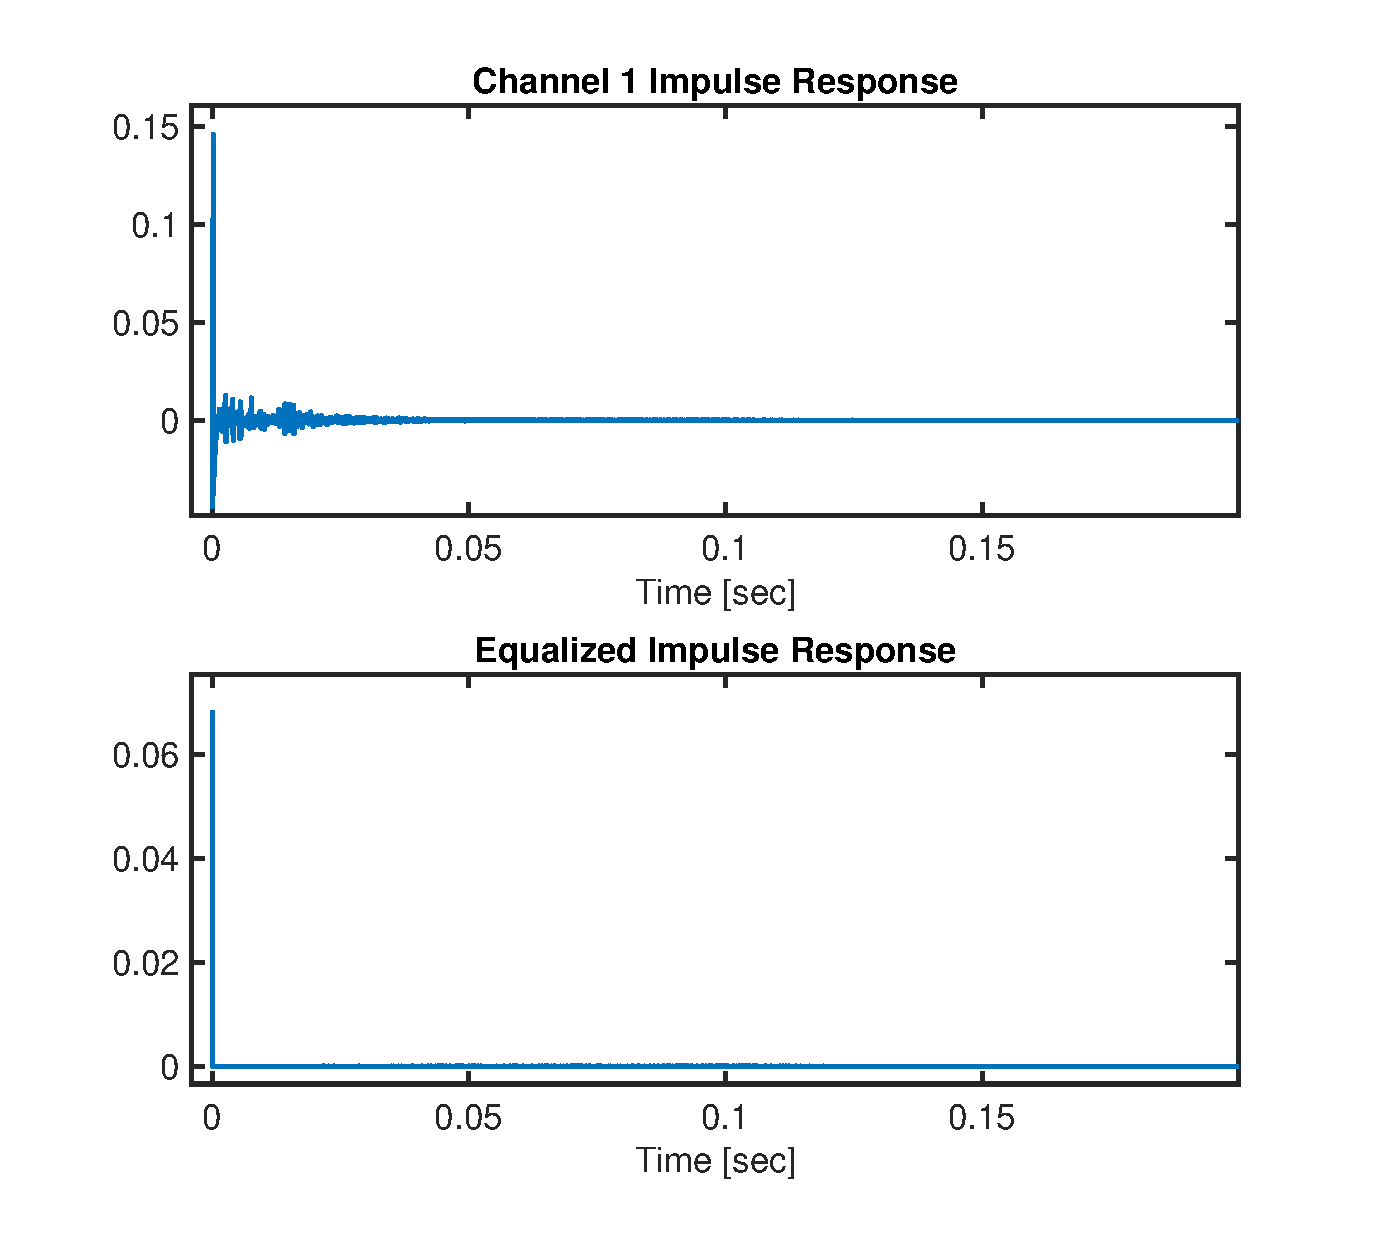
\includegraphics[width=\textwidth]{EIR_0p75N60_div_M_minus_1}
	\end{subfigure}
	\begin{subfigure}[b]{0.4\textwidth}
		\centering
		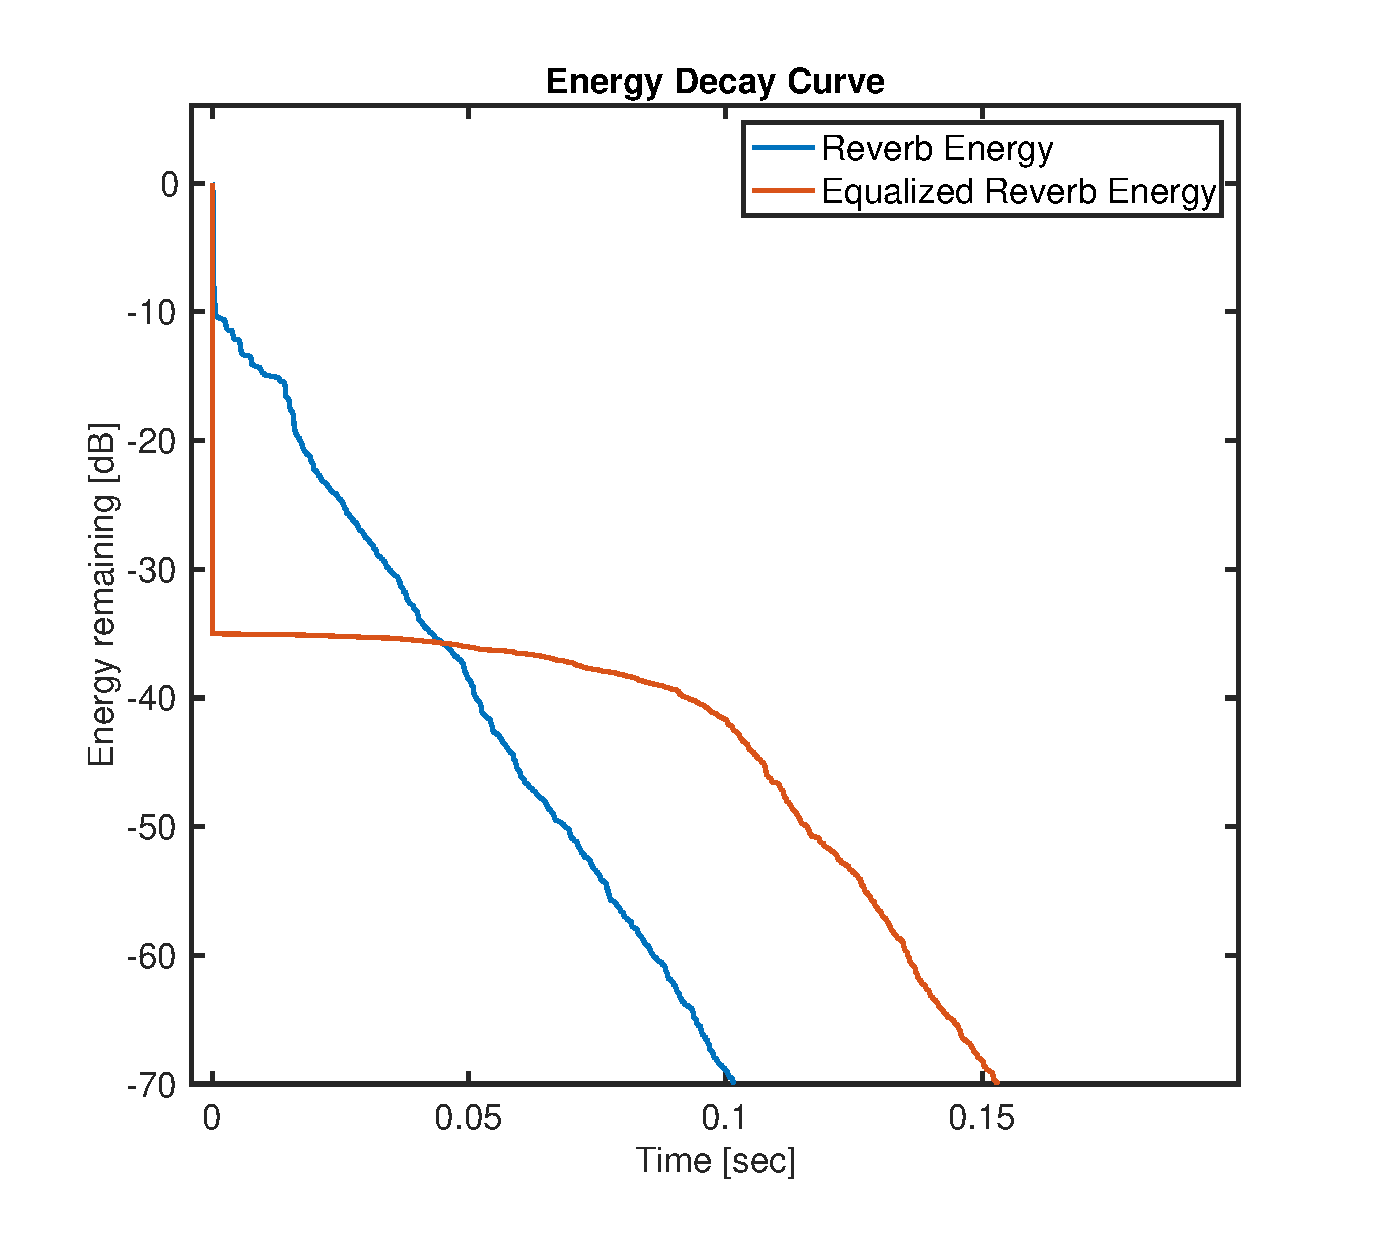
\includegraphics[width=\textwidth]{EDC_0p75N60_div_M_minus_1}
	\end{subfigure}
	\begin{subfigure}[b]{0.4\textwidth}
		\centering
		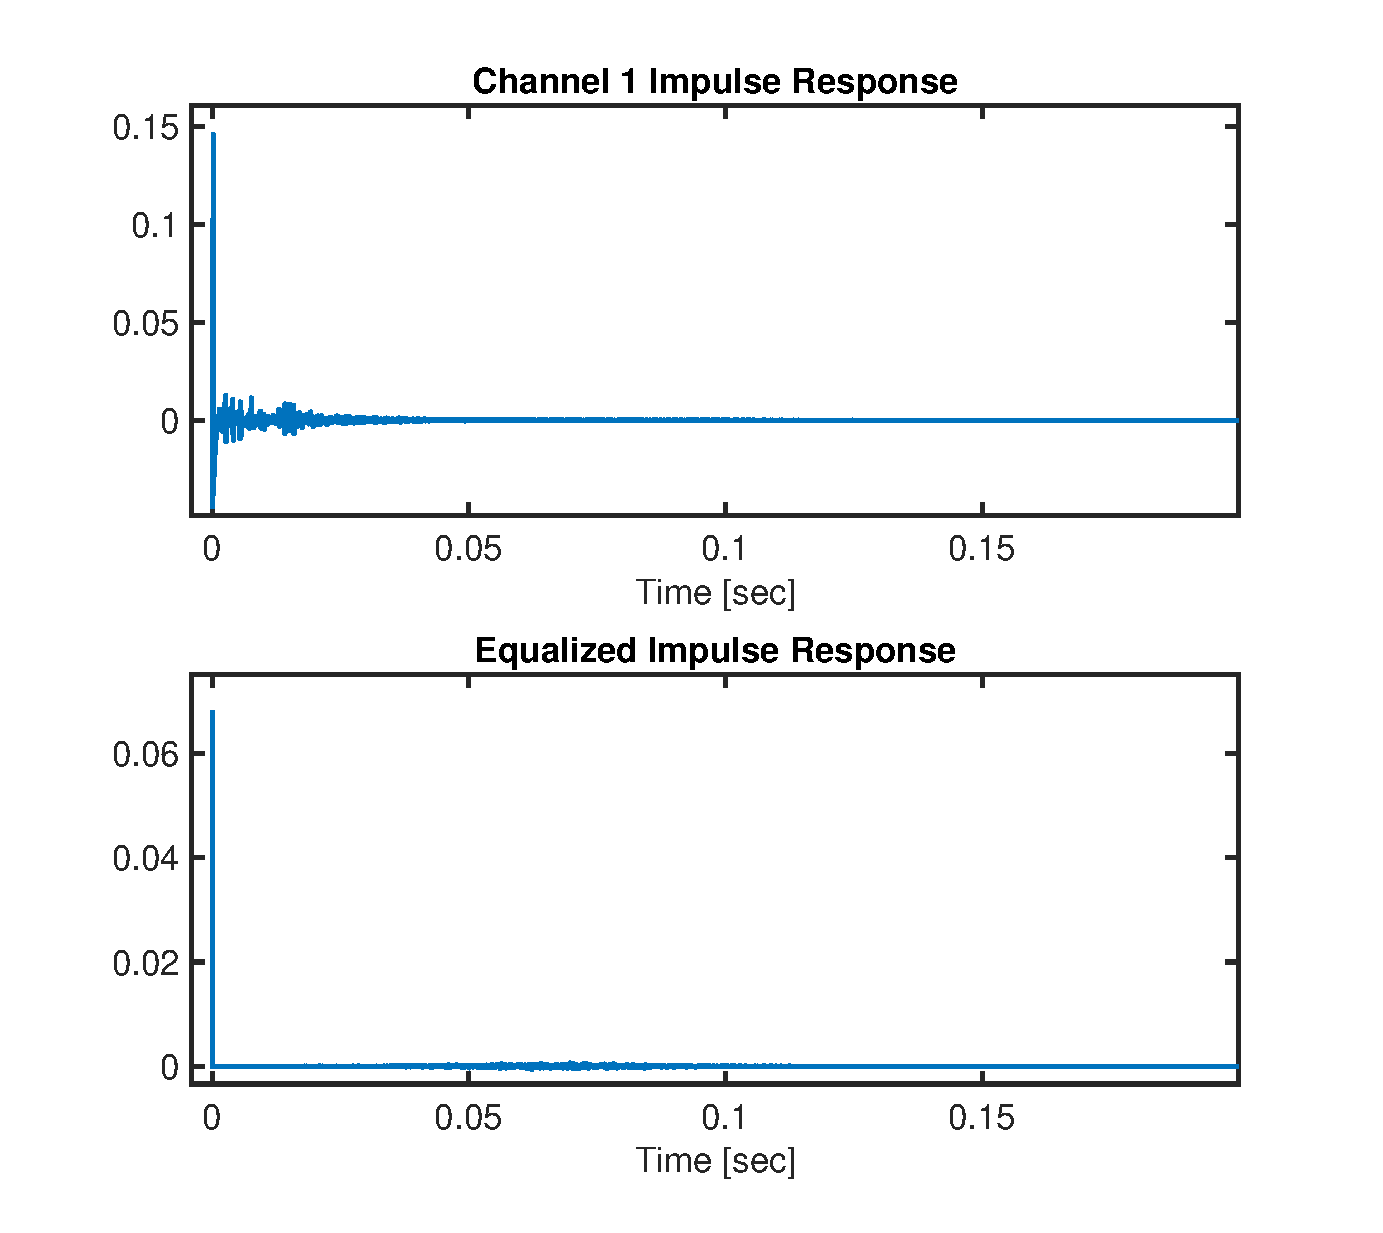
\includegraphics[width=\textwidth]{EIR_0p5N60_div_M_minus_1}
	\end{subfigure}
	\begin{subfigure}[b]{0.4\textwidth}
		\centering
		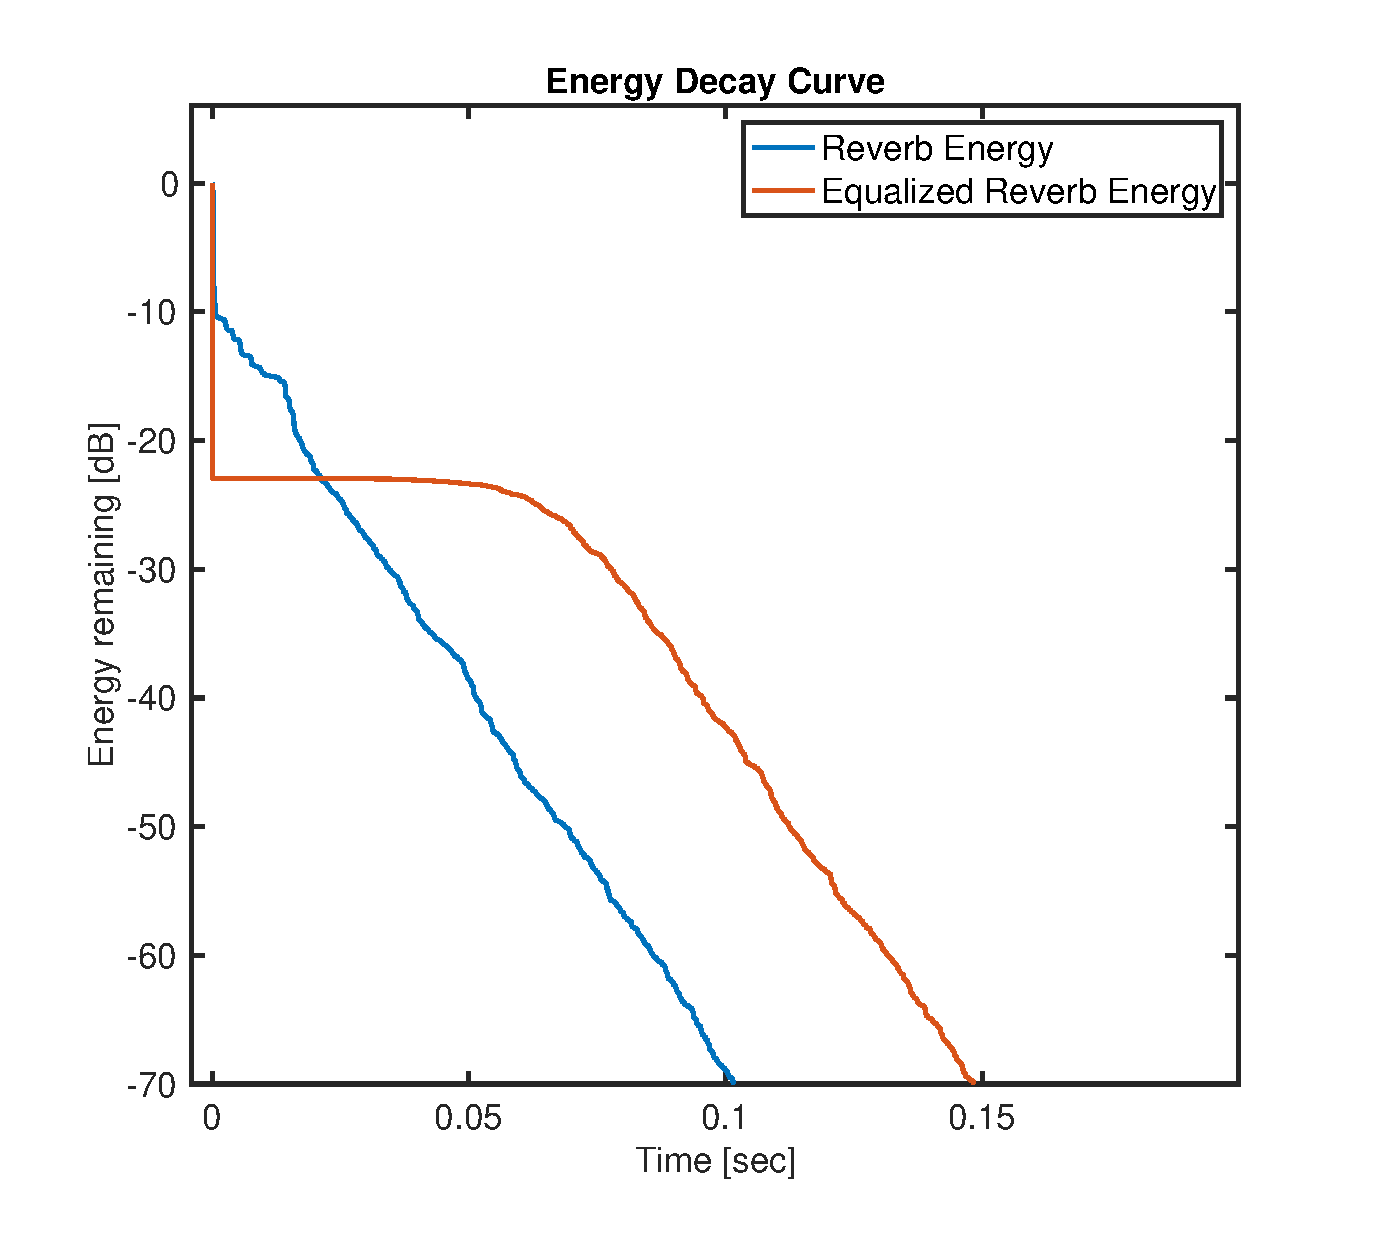
\includegraphics[width=\textwidth]{EDC_0p5N60_div_M_minus_1}
	\end{subfigure}
	\caption{Delay-and-Predict dereverberation performance with various multichannel linear prediction orders ($\mathrm{p2}$) relative to the actual length of the FIR channel ($L$) and the number of samples corresponding to the T60 of the channel ($\mathrm{N60}$). Figure \ref{fig:params_p2_stage1} shows the common source whitening filter used.}
	\label{fig:params_p2_compare}
\end{figure}

\section{Source Whitening Linear Prediction Order}


Test Conditions:
- Source Signal = SA1.WAV
- Source length = 348366
- RIR = MYRiAD SAL Measured RIR (T60 = 2100 msec, Truncated Exponentially to T60 = 100 msec)
- RIR length = 3200
- T60 = 100 msec (N60 = 1600 samples)
- SNR = 300 dB
- Noise Signal = office ventilation
- SIR = Inf dB
- Interference Signal = None

Delay-and-Predict config:
- Number of Microphones (M) = 4
- Source whitening order (p1) = varied
- Multichannel Linear Prediction order (p2) = 533 (N60 / (M-1))
- Source whitening Enabled? = 1
- Source whitening on clean speech? = 1

\textbf{p1 = 200 (Original Paper)}

\begin{figure}[H]
	\centering
	\begin{subfigure}[b]{0.49\textwidth}
		\centering
		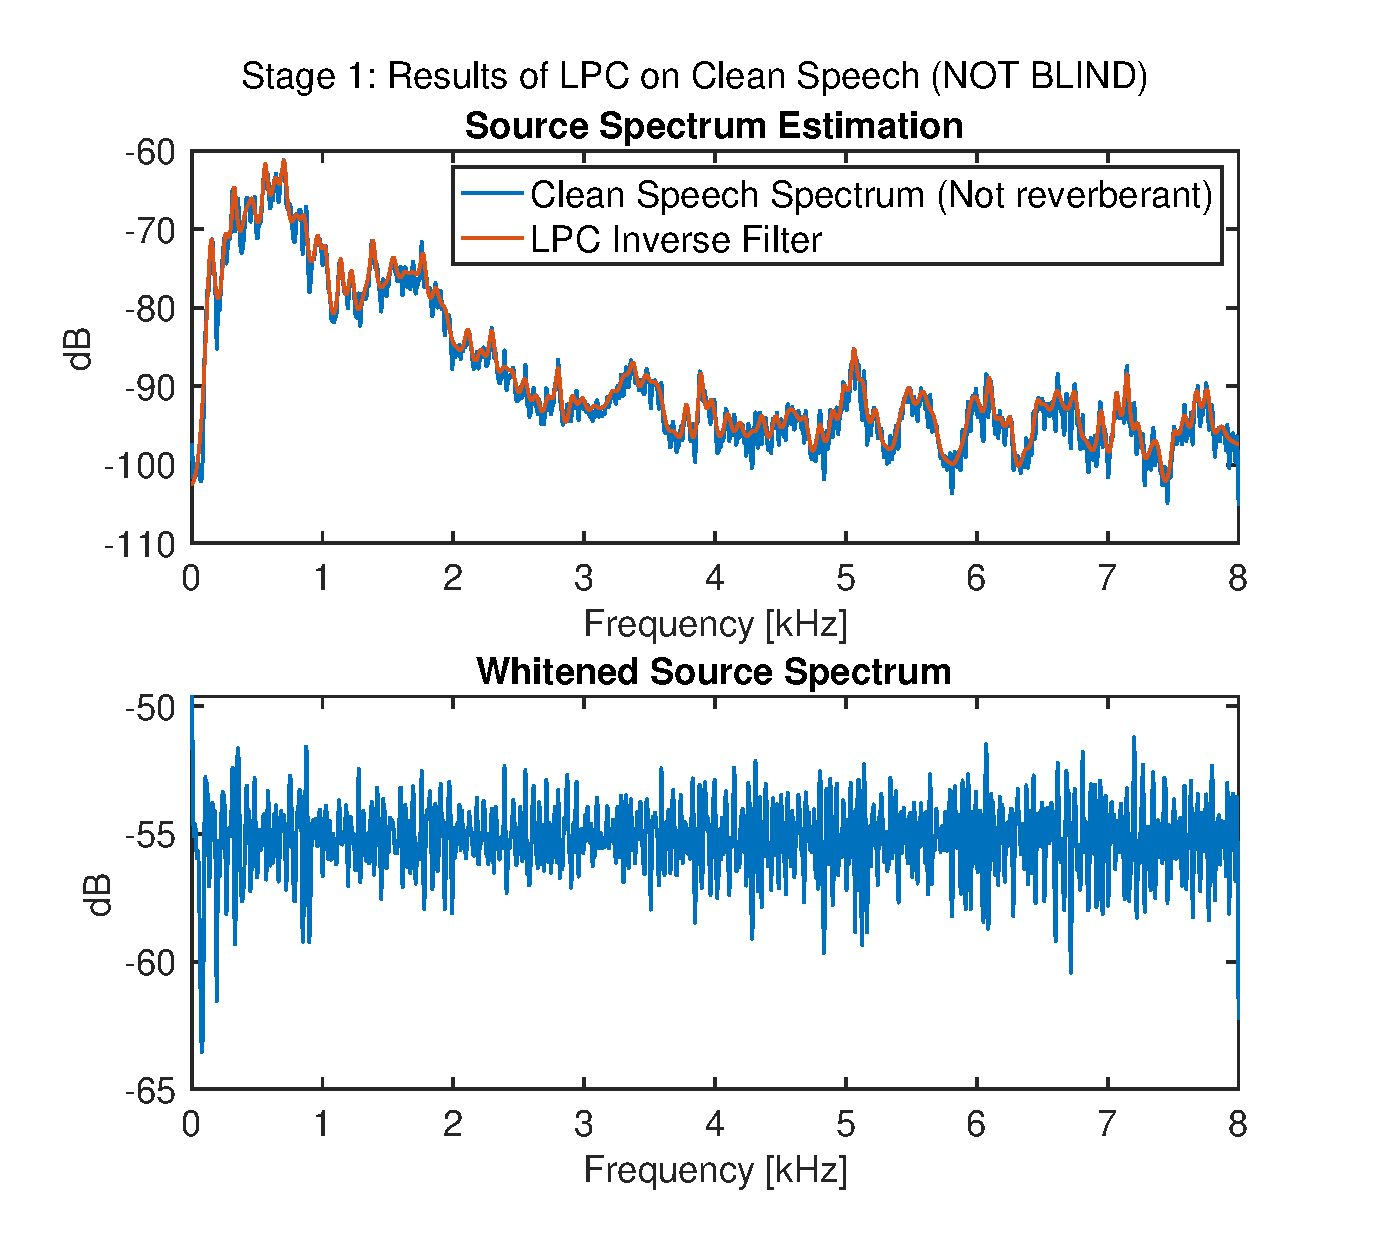
\includegraphics[width=\textwidth]{S1_p1_200}
	\end{subfigure}
	\hfill
	\begin{subfigure}[b]{0.49\textwidth}
		\centering
		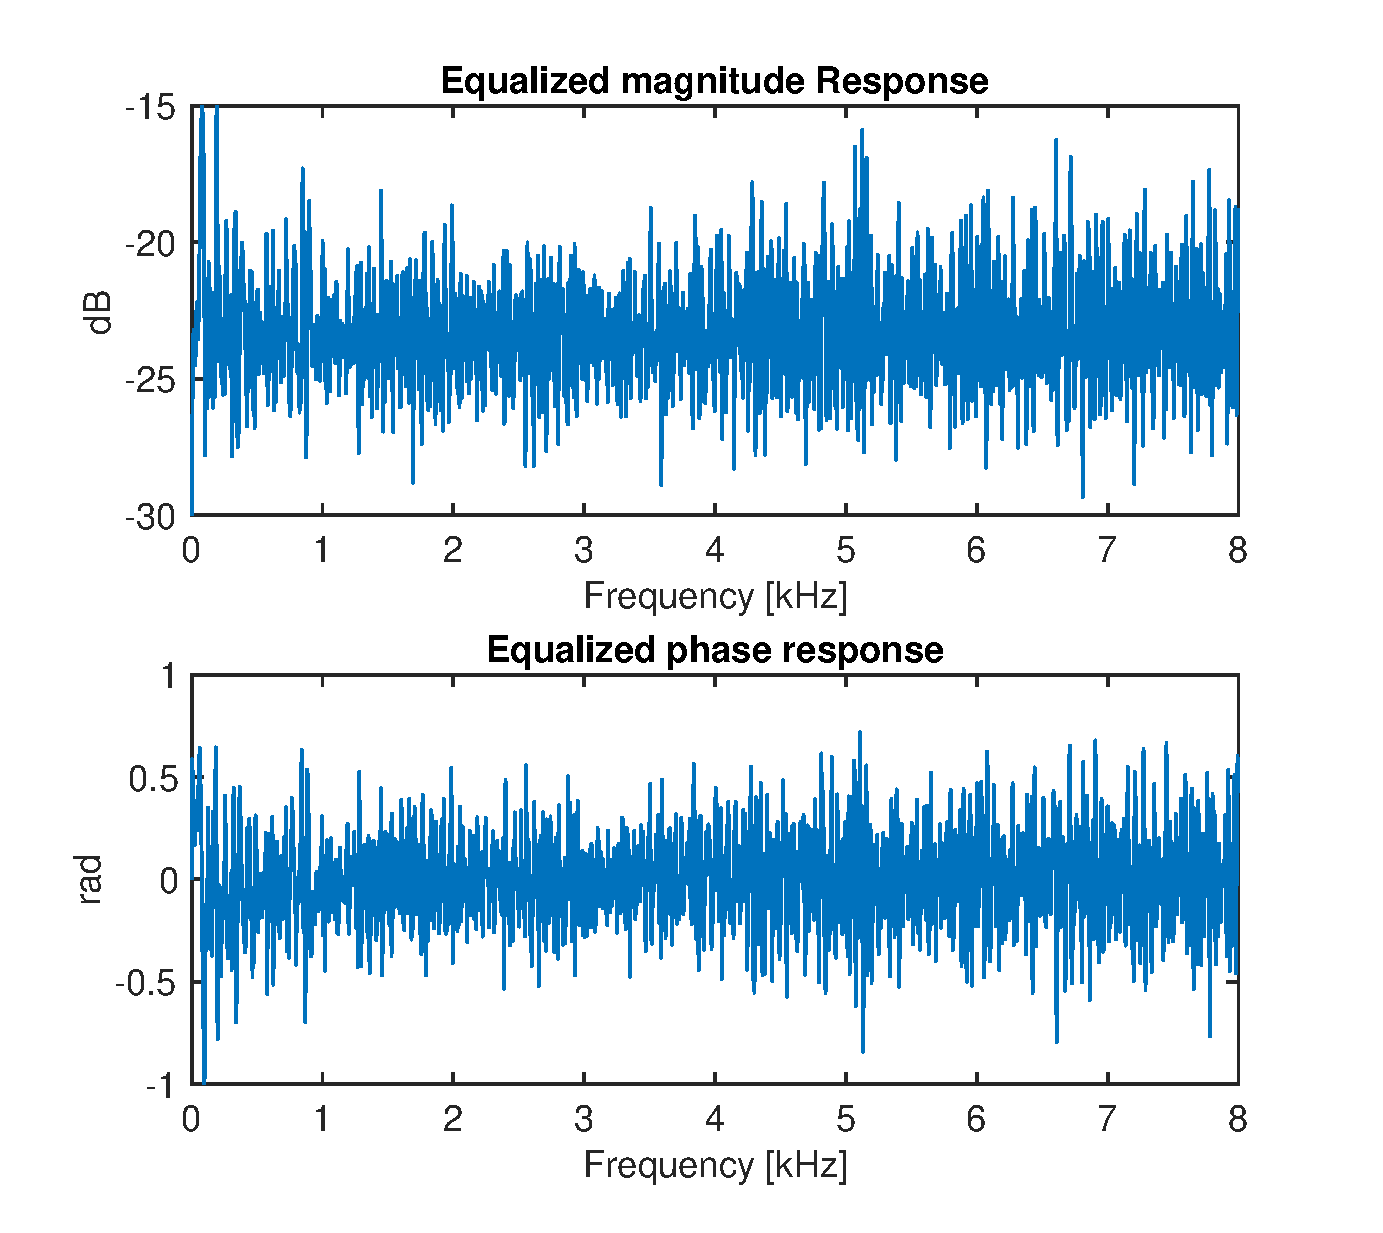
\includegraphics[width=\textwidth]{Equalized_RTF_p1_200}
	\end{subfigure}
	\hfill
	\begin{subfigure}[b]{0.49\textwidth}
		\centering
		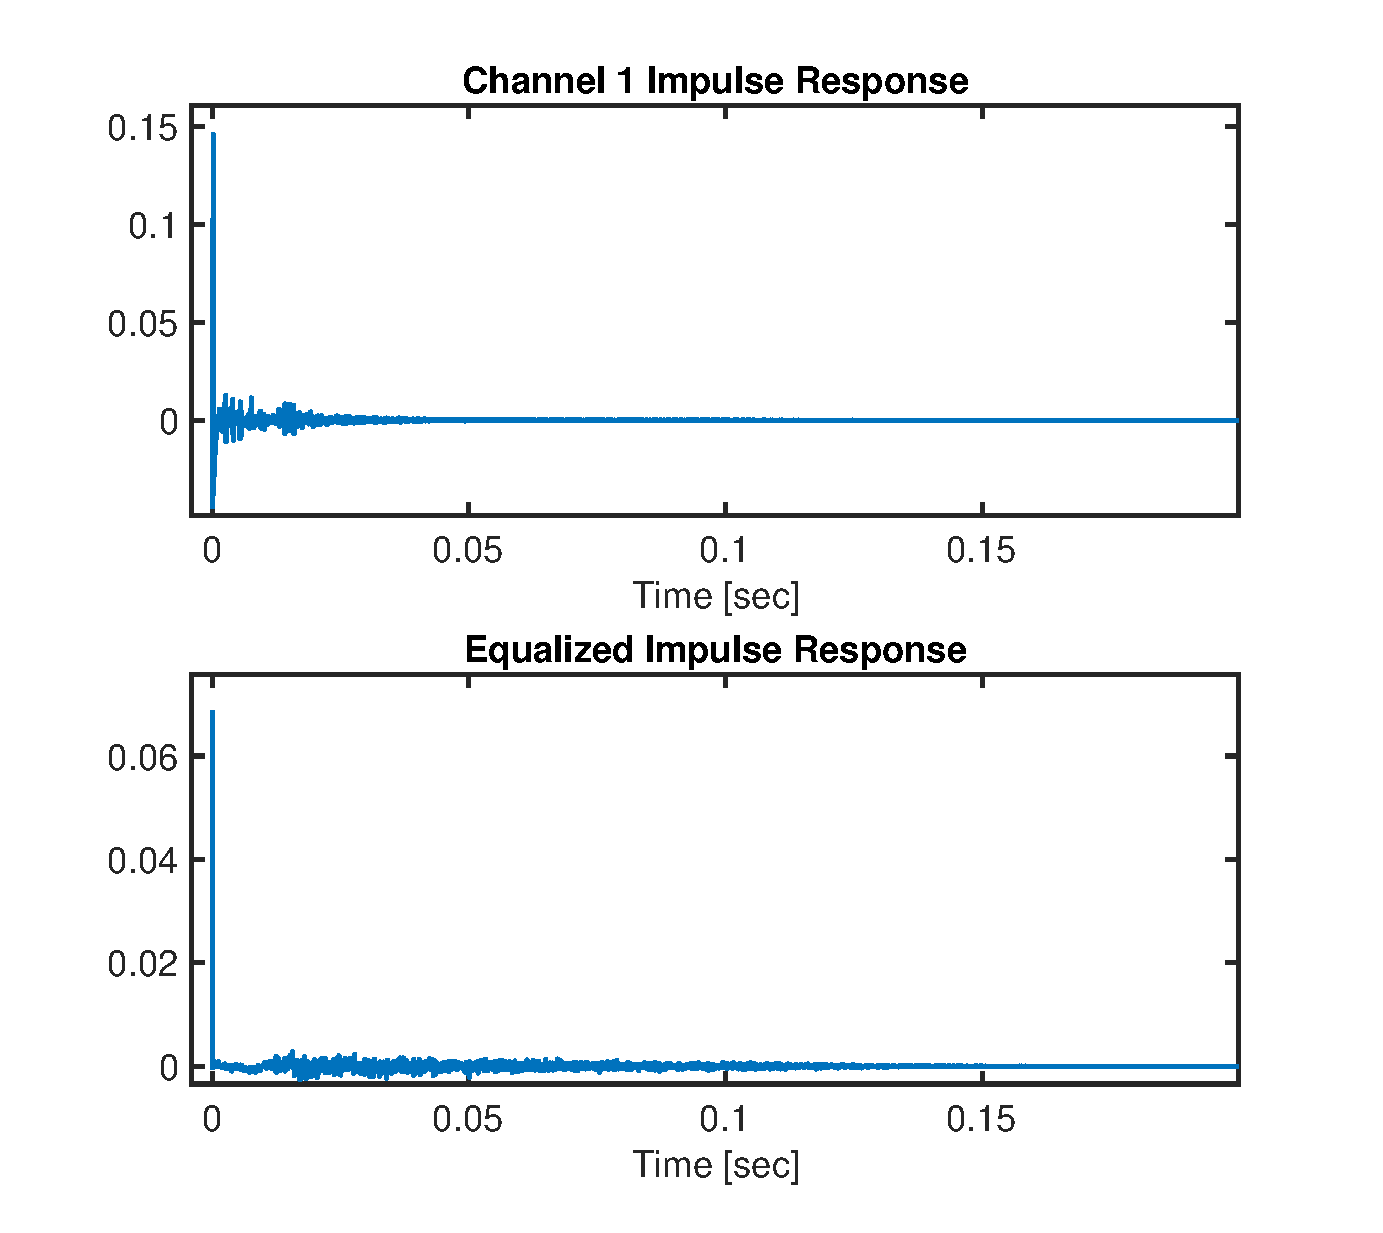
\includegraphics[width=\textwidth]{EIR_p1_200}
	\end{subfigure}
	\hfill
	\begin{subfigure}[b]{0.49\textwidth}
		\centering
		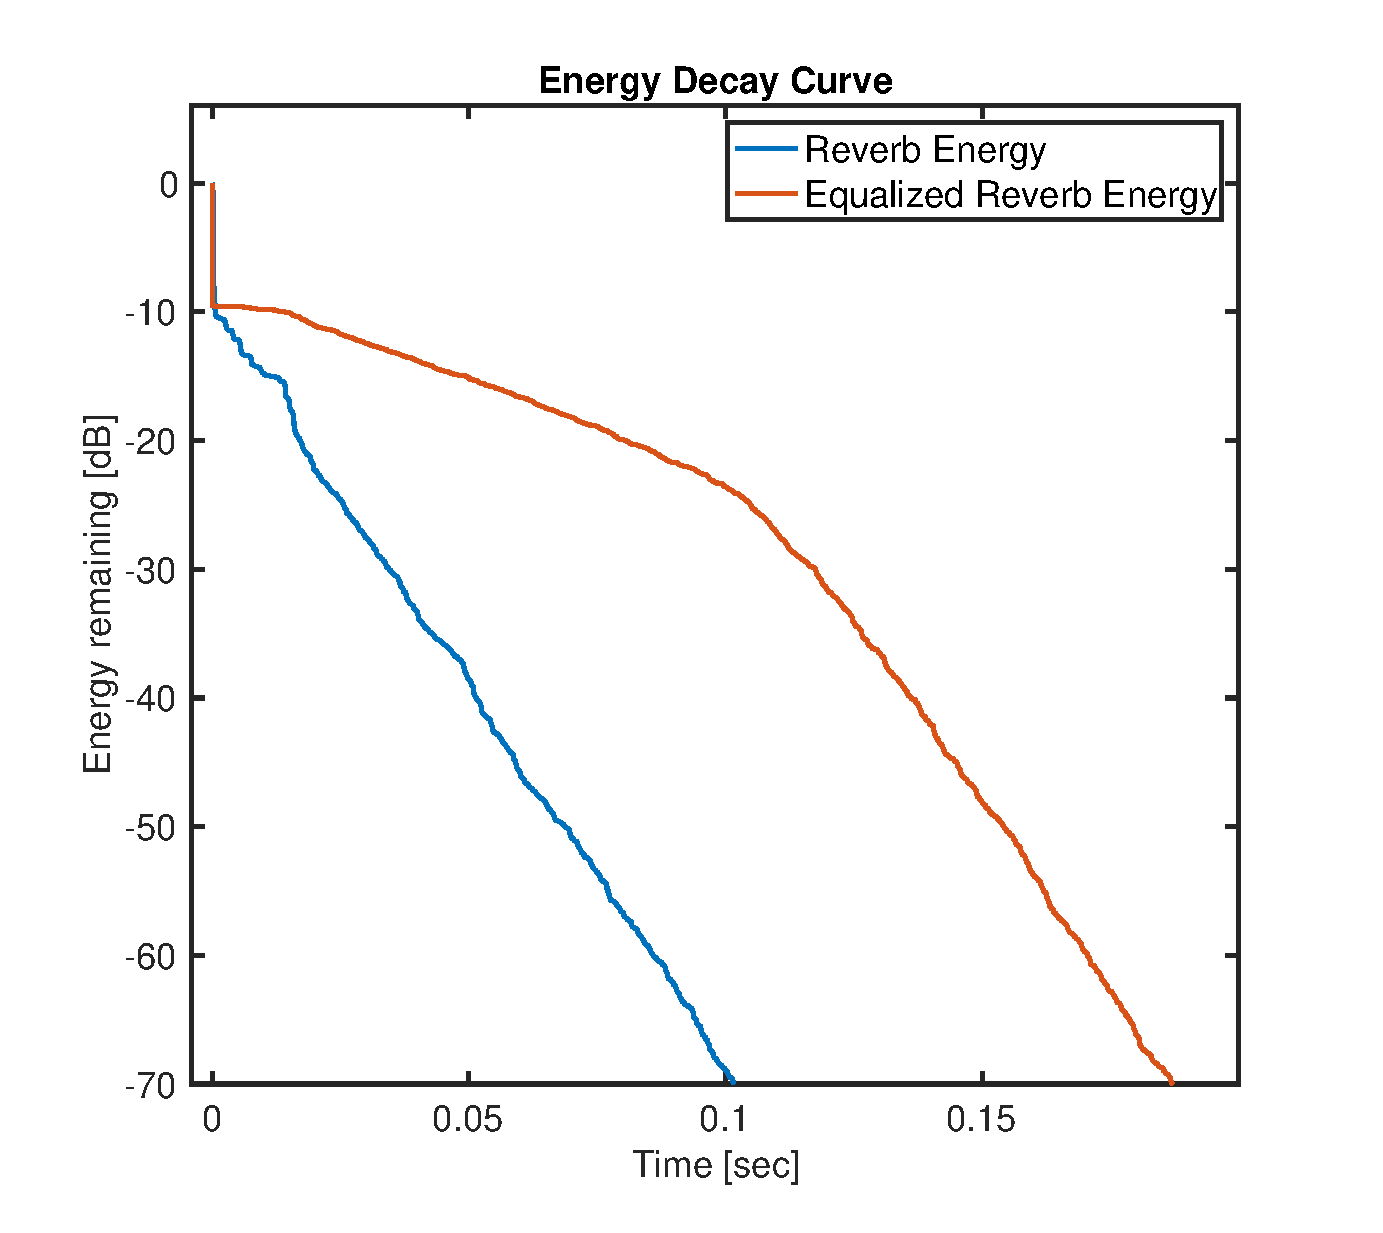
\includegraphics[width=\textwidth]{EDC_p1_200}
	\end{subfigure}
	\hfill
	\caption{Delay-and-Predict dereverberation performance with source whitening prediction order $\mathrm{p1} = 200$ and multichannel linear prediction order $\mathrm{p2} = N60 / (M-1)$.}
	\label{fig:params_p1_200}
\end{figure}

\textbf{Comparison: p1 = [200  1000  p2*(M-1)  2*p2*(M-1)]}

\begin{figure}[H]
	\centering
	\begin{subfigure}[b]{0.4\textwidth}
		\centering
		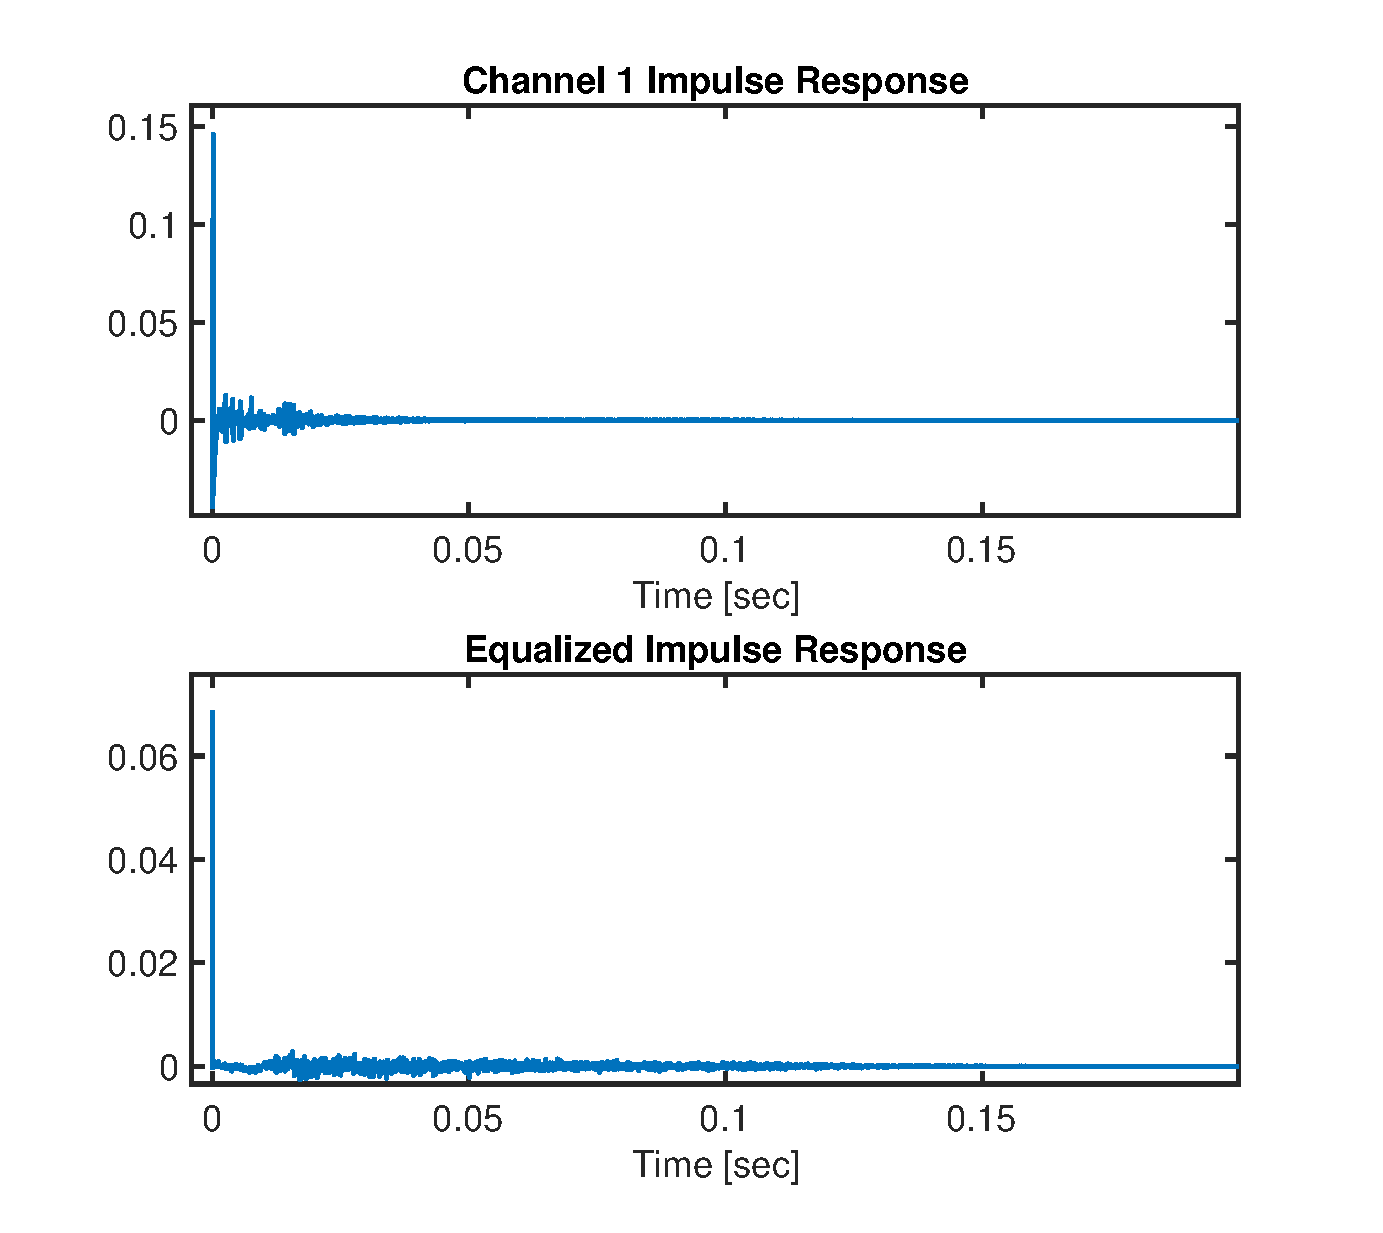
\includegraphics[width=\textwidth]{EIR_p1_200}
	\end{subfigure}
	\begin{subfigure}[b]{0.4\textwidth}
		\centering
		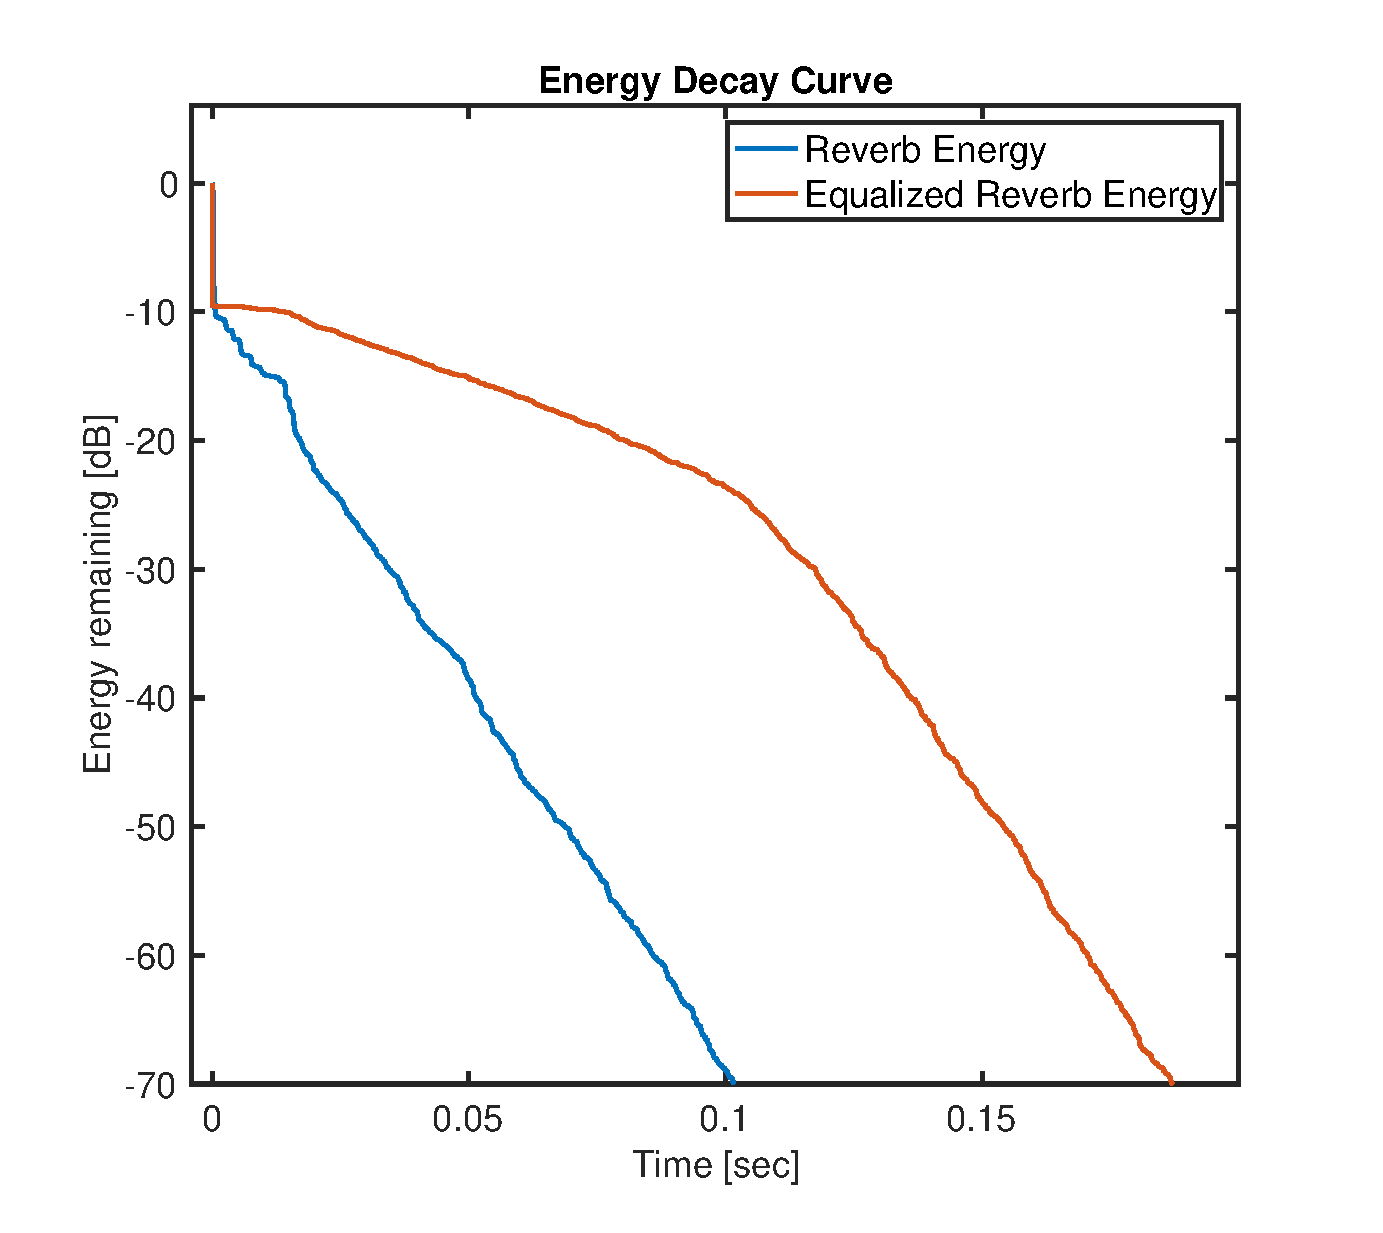
\includegraphics[width=\textwidth]{EDC_p1_200}
	\end{subfigure}
	\begin{subfigure}[b]{0.4\textwidth}
		\centering
		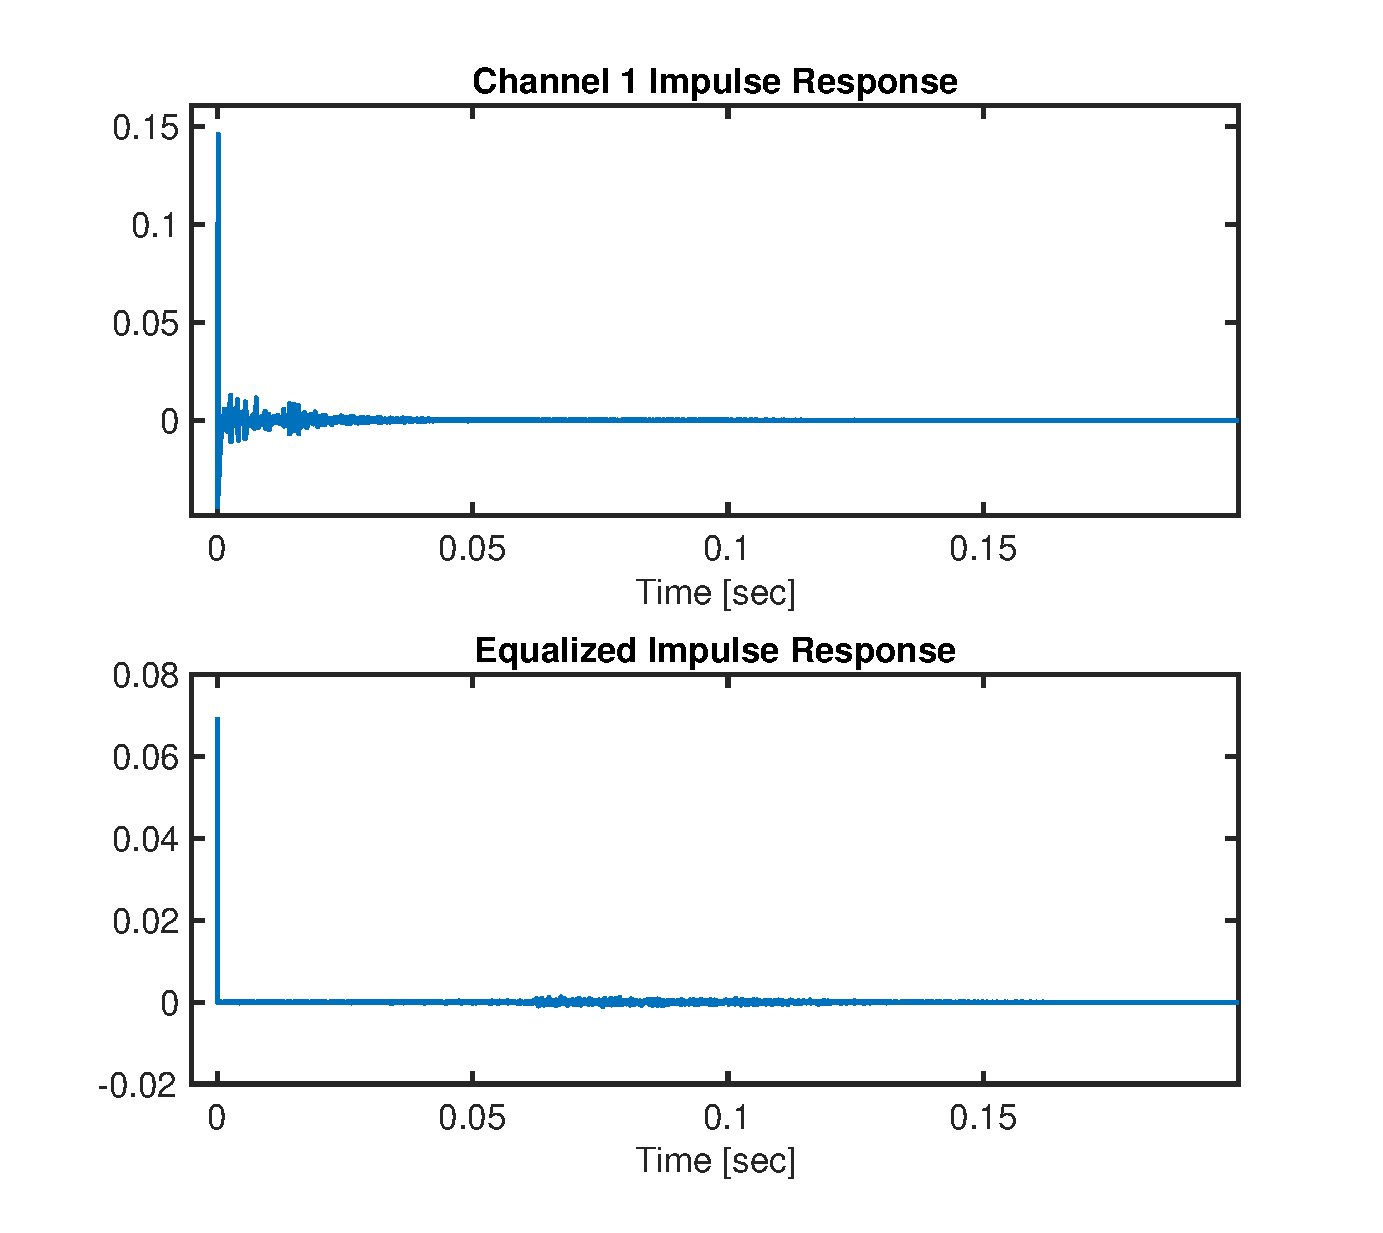
\includegraphics[width=\textwidth]{EIR_p1_1000}
	\end{subfigure}
	\begin{subfigure}[b]{0.4\textwidth}
		\centering
		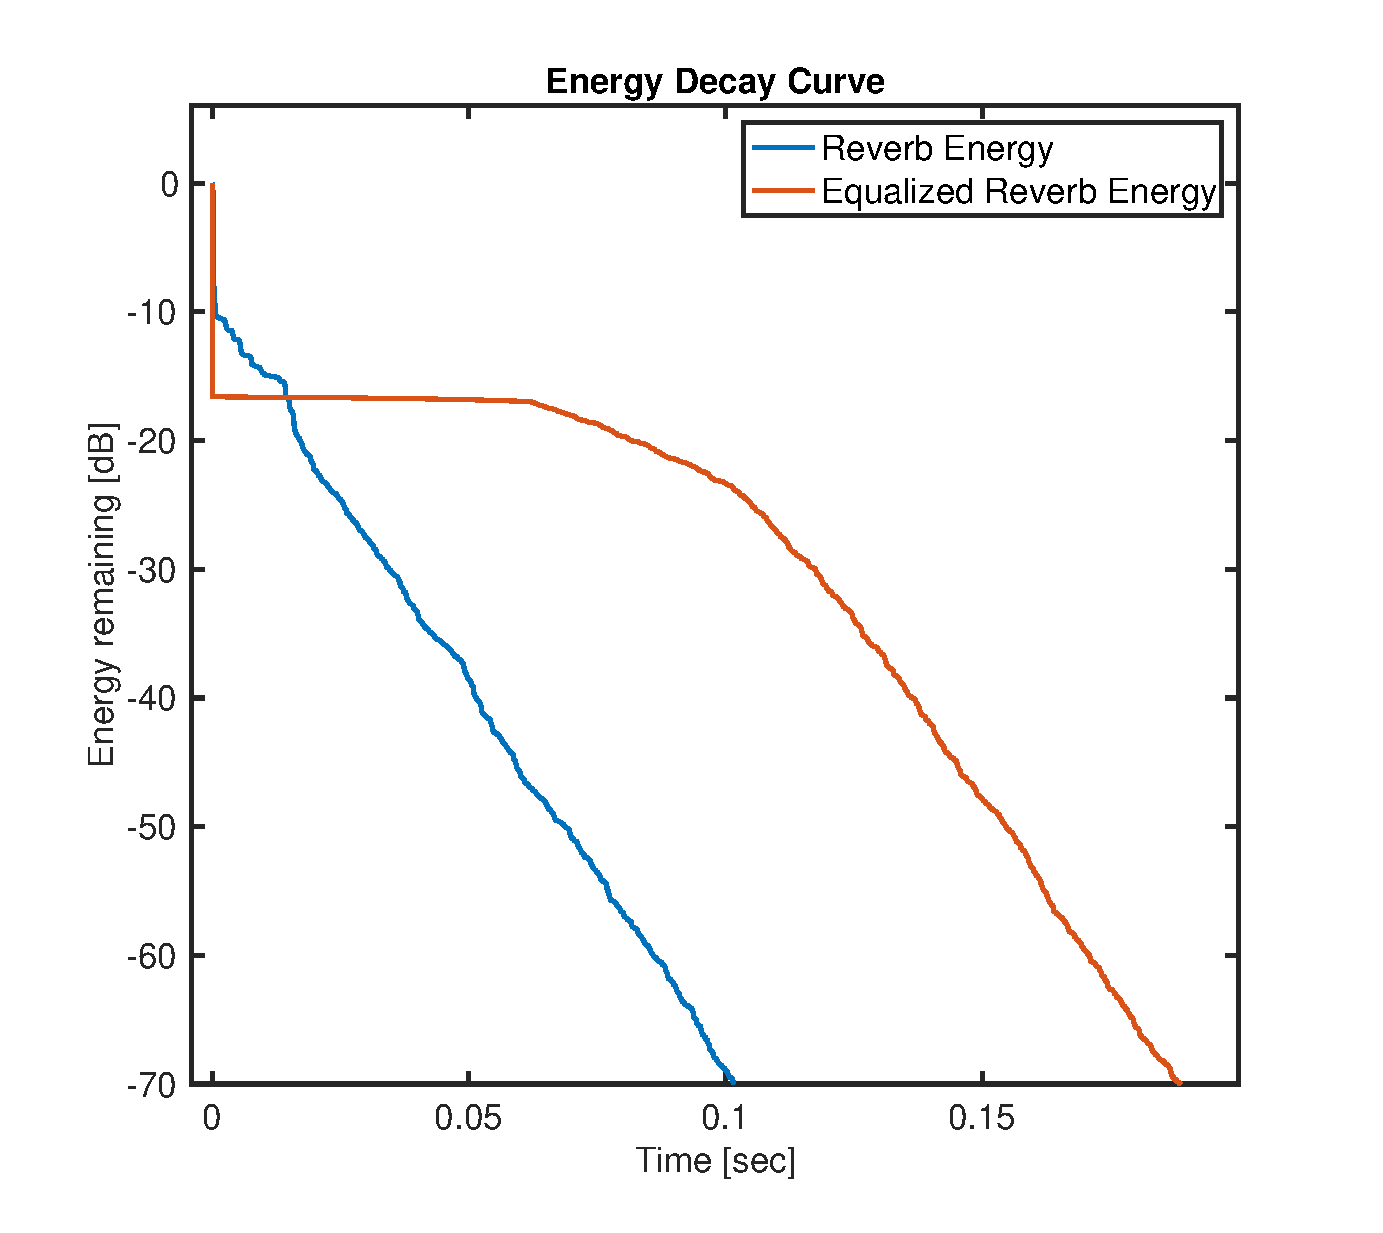
\includegraphics[width=\textwidth]{EDC_p1_1000}
	\end{subfigure}
	\begin{subfigure}[b]{0.4\textwidth}
		\centering
		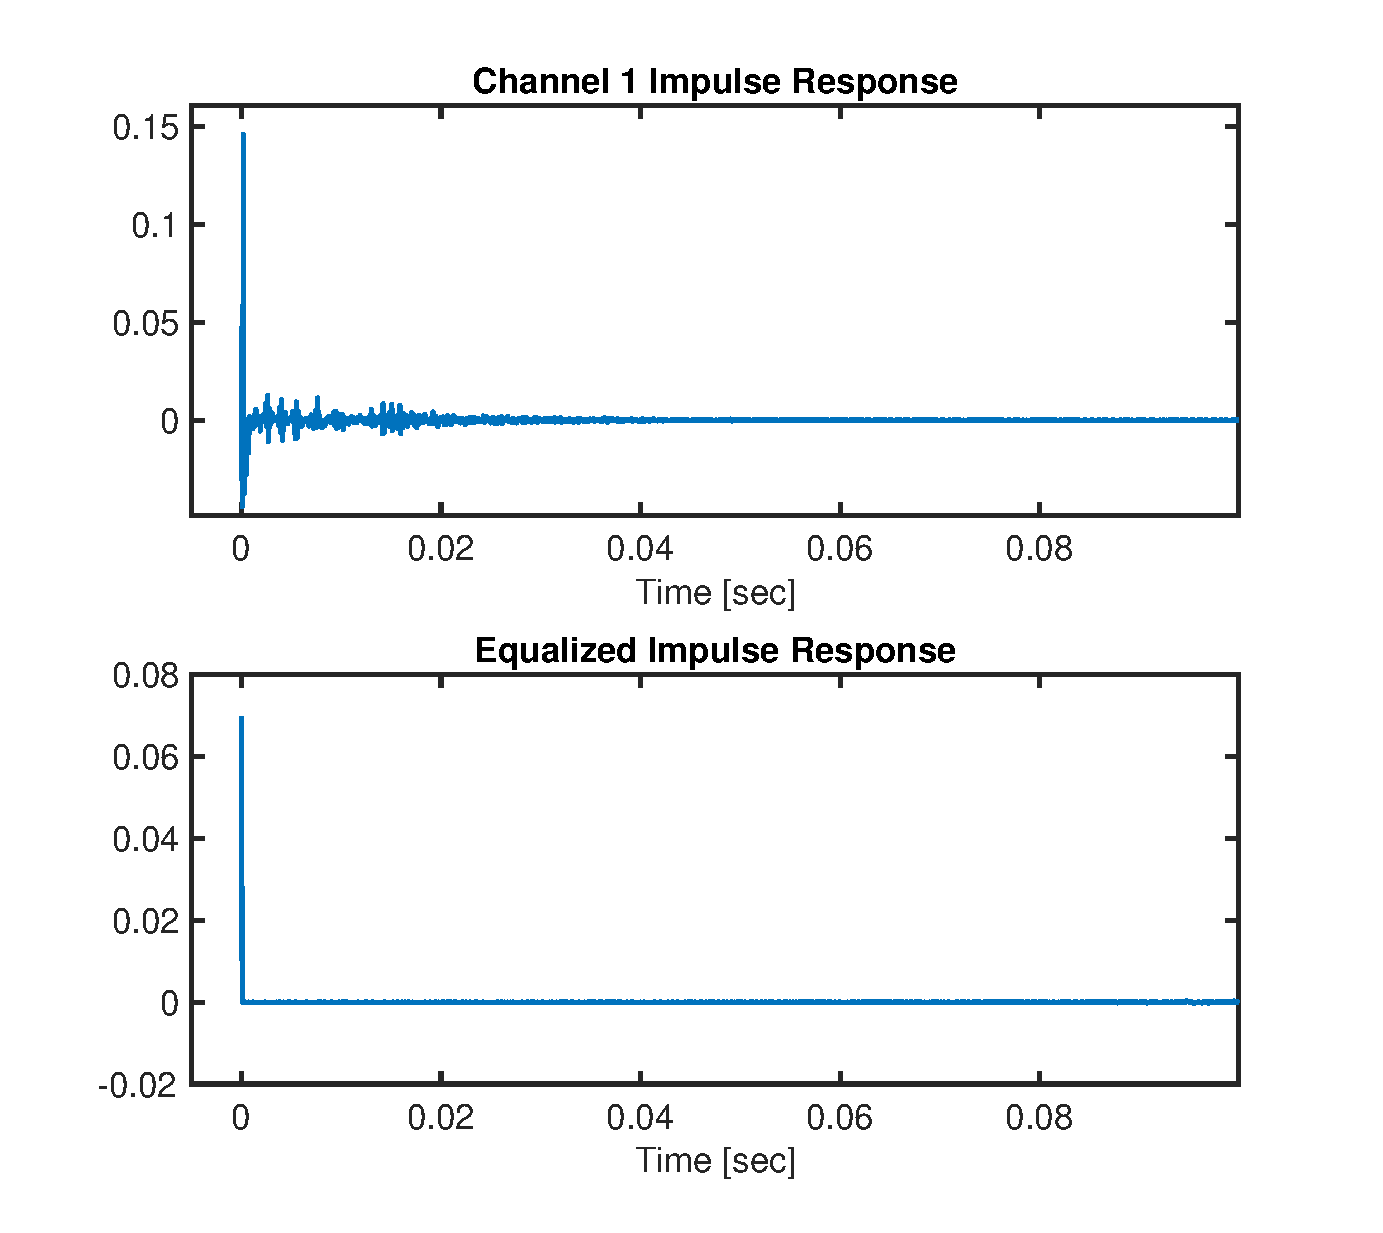
\includegraphics[width=\textwidth]{EIR_p1_based_on_p2}
	\end{subfigure}
	\begin{subfigure}[b]{0.4\textwidth}
		\centering
		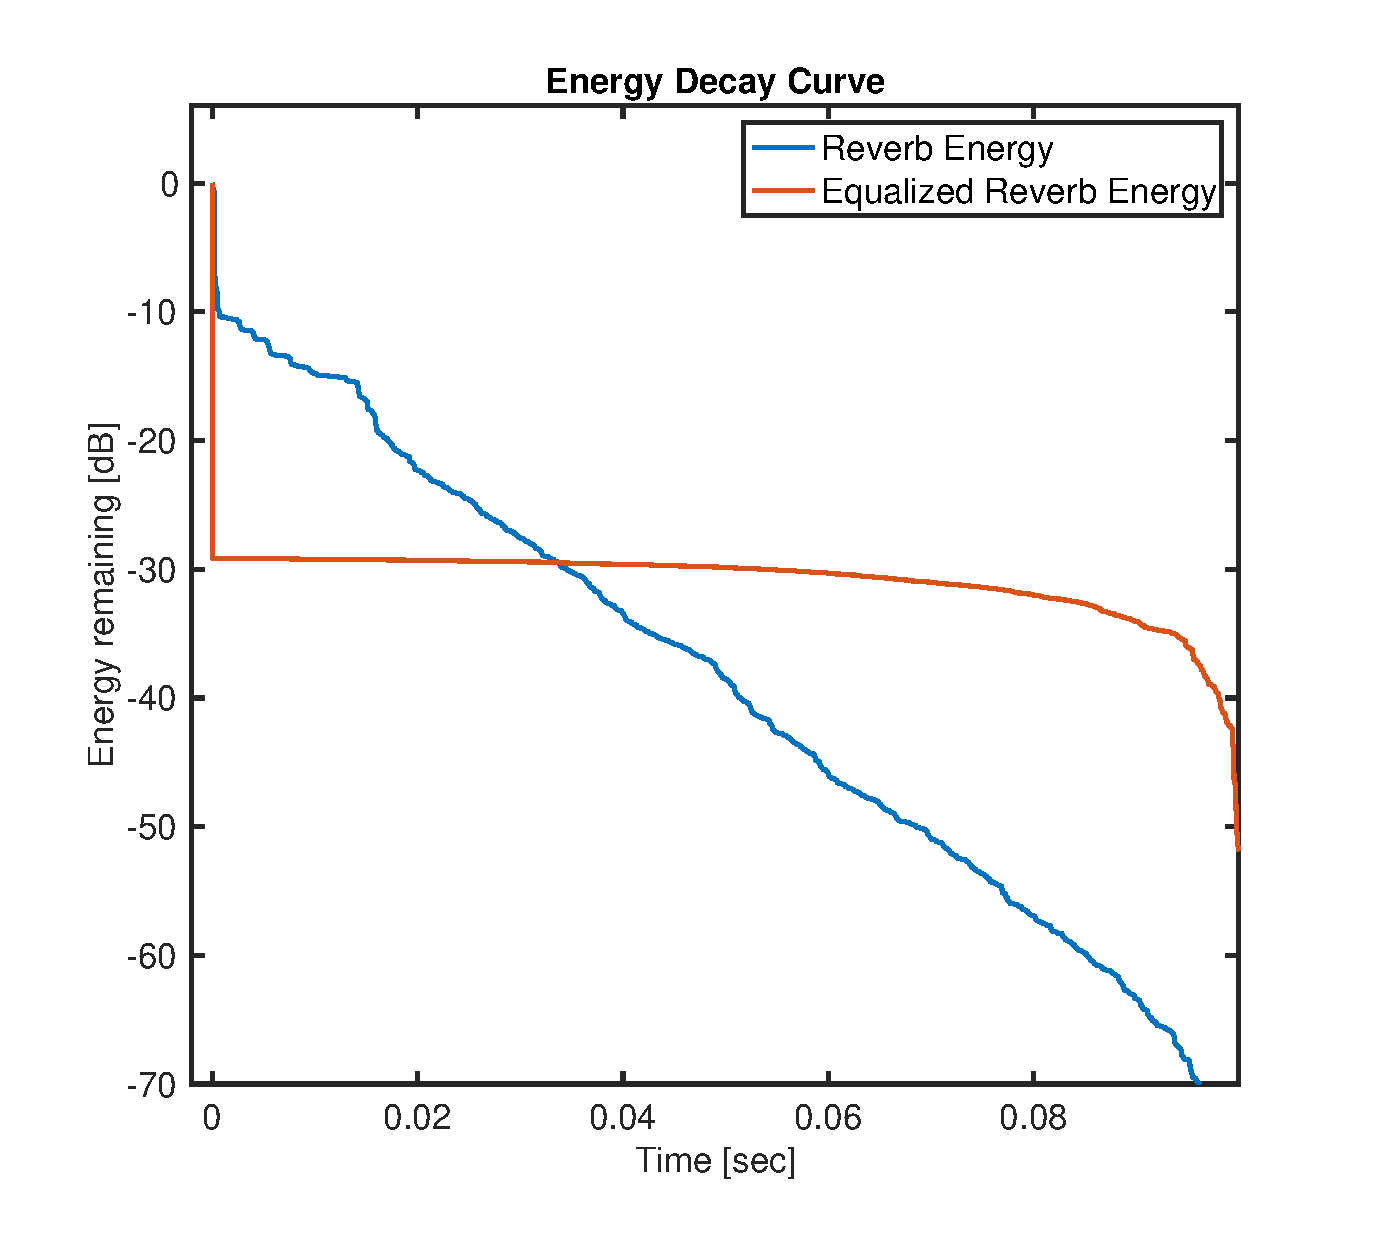
\includegraphics[width=\textwidth]{EDC_p1_based_on_p2}
	\end{subfigure}
	\begin{subfigure}[b]{0.4\textwidth}
		\centering
		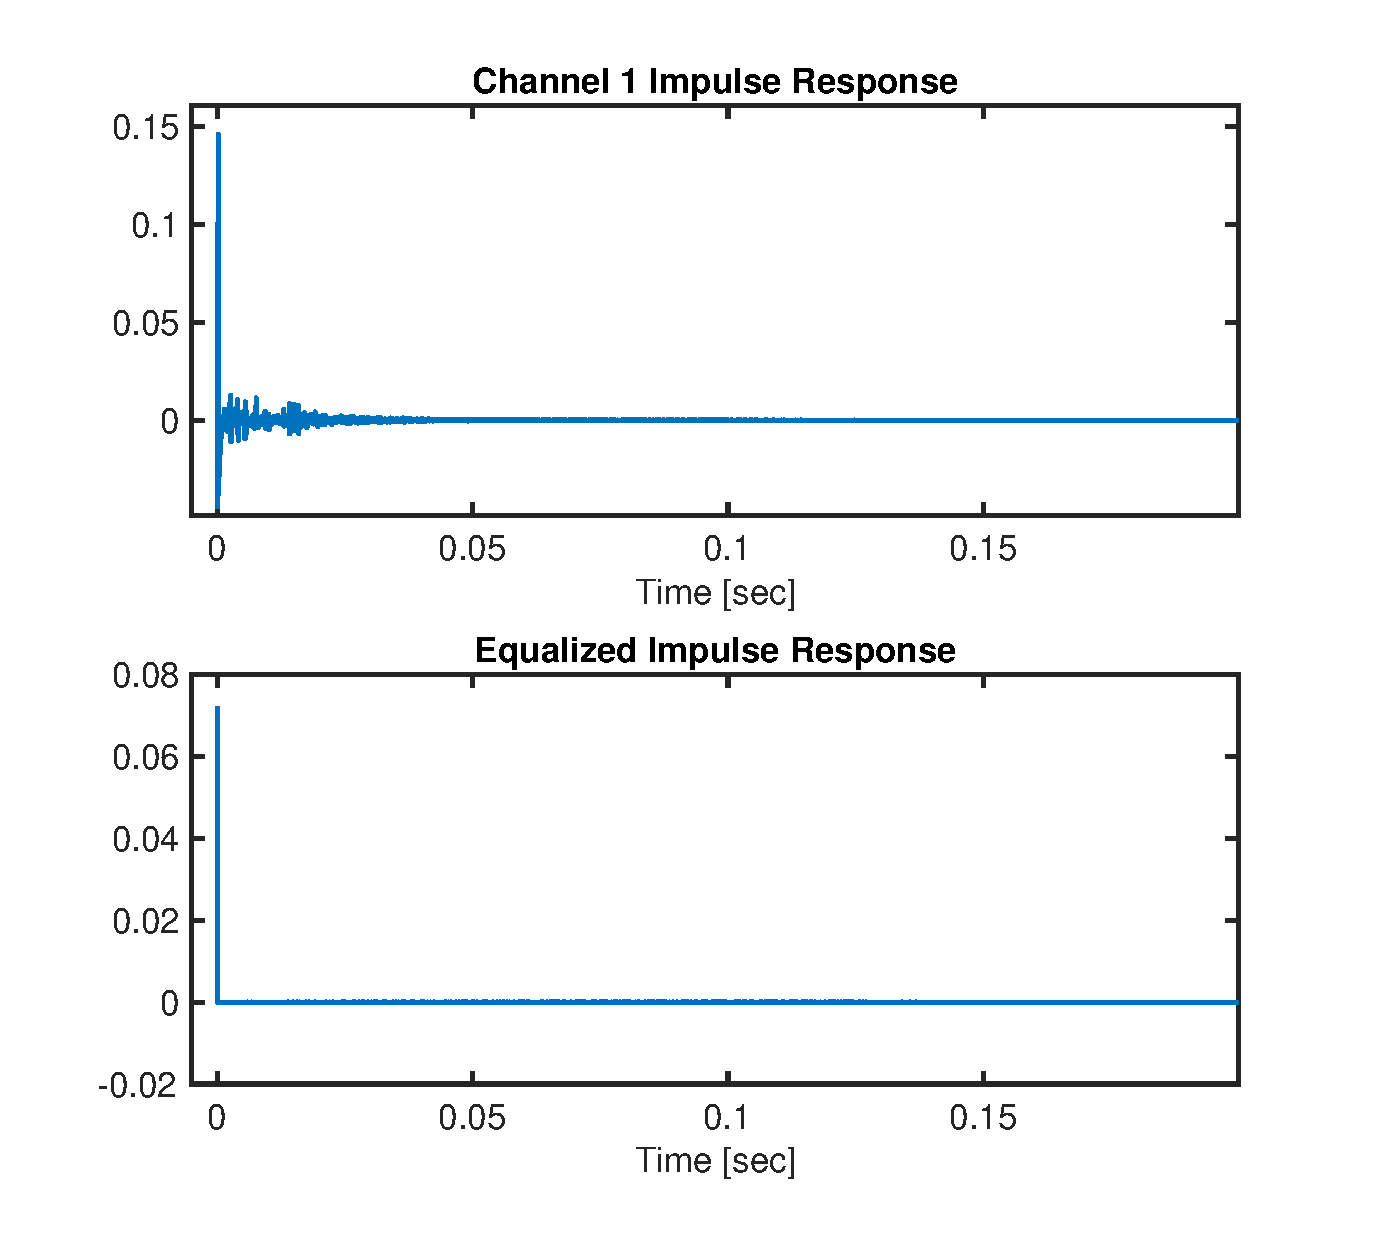
\includegraphics[width=\textwidth]{EIR_p1_2x_p2}
	\end{subfigure}
	\begin{subfigure}[b]{0.4\textwidth}
		\centering
		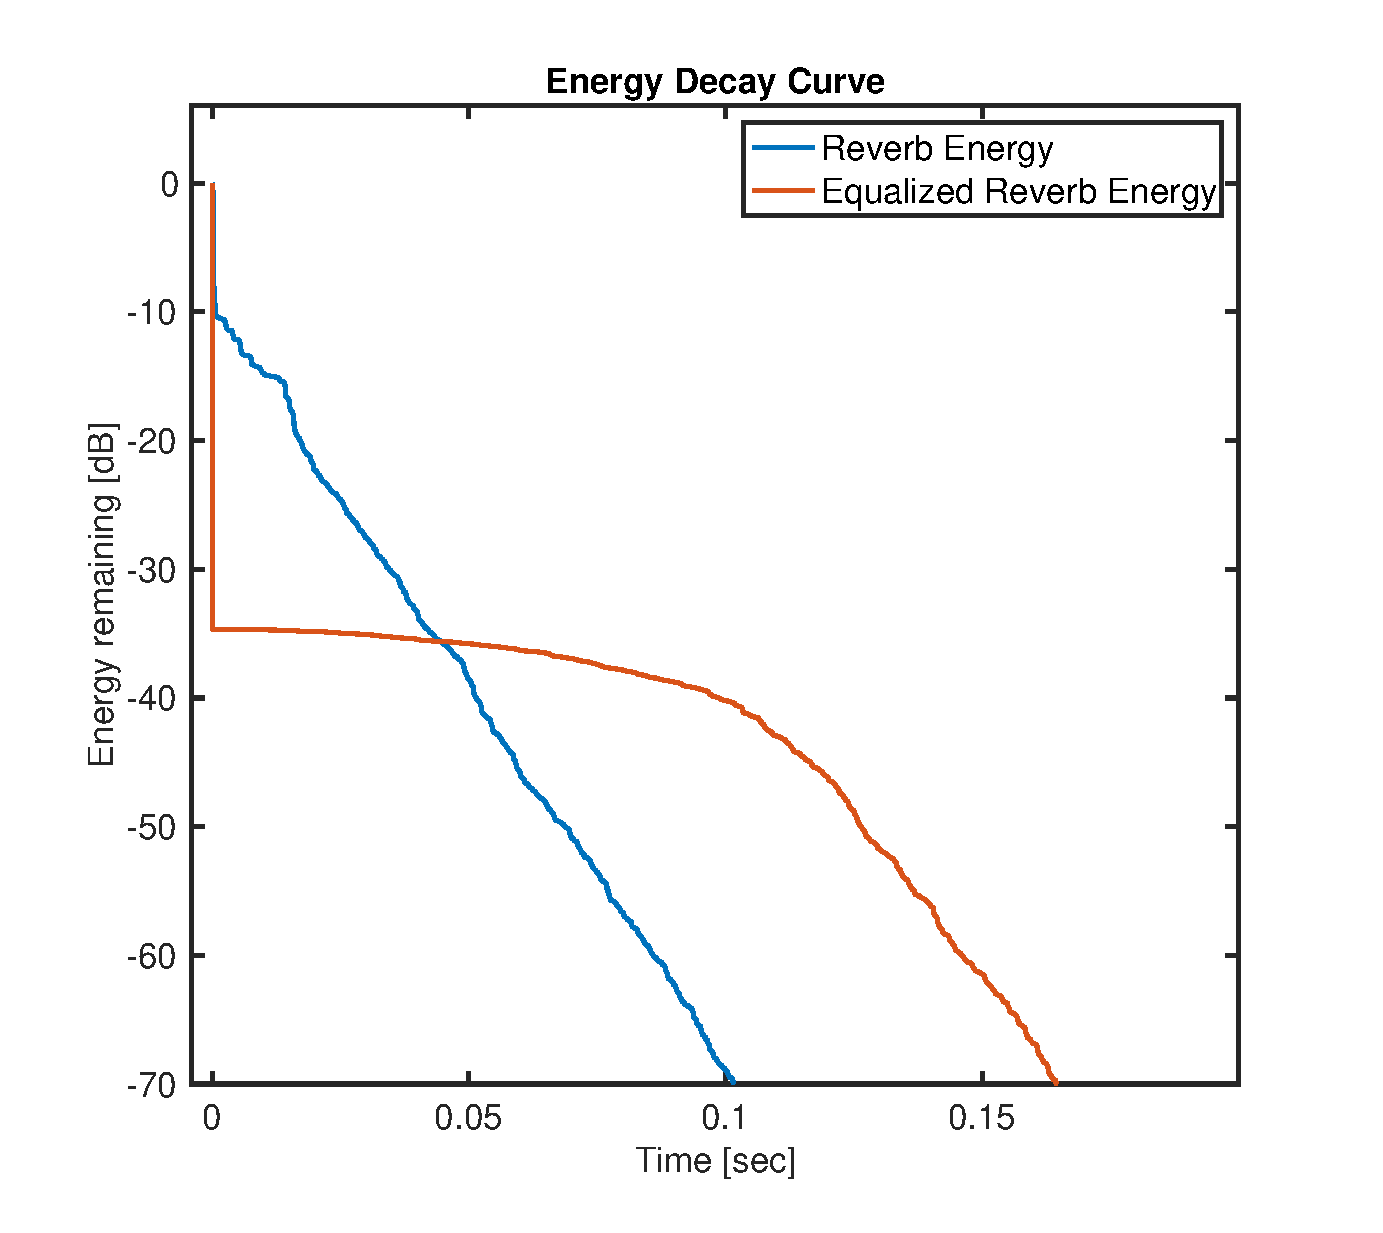
\includegraphics[width=\textwidth]{EDC_p1_2x_p2}
	\end{subfigure}
	\caption{Delay-and-Predict dereverberation performance with various source whitening prediction orders (p1) relative to the multichannel linear prediction order $\mathrm{p2} = \mathrm{N60} / (M-1)$}
	\label{fig:params_p1_compare}
\end{figure}


... beyond about p1 = 1.25 * p2 * (M-1) EDC performance saturates at approximately -35 dB reverb attenuation.



\section{Blind Deconvolution Performance}

Compare Spectrogram/EDC of Blind DAP, Supervised DAP and MINT

\begin{figure}[H]
	\centering
	\begin{subfigure}[b]{0.38\textwidth}
		\centering
		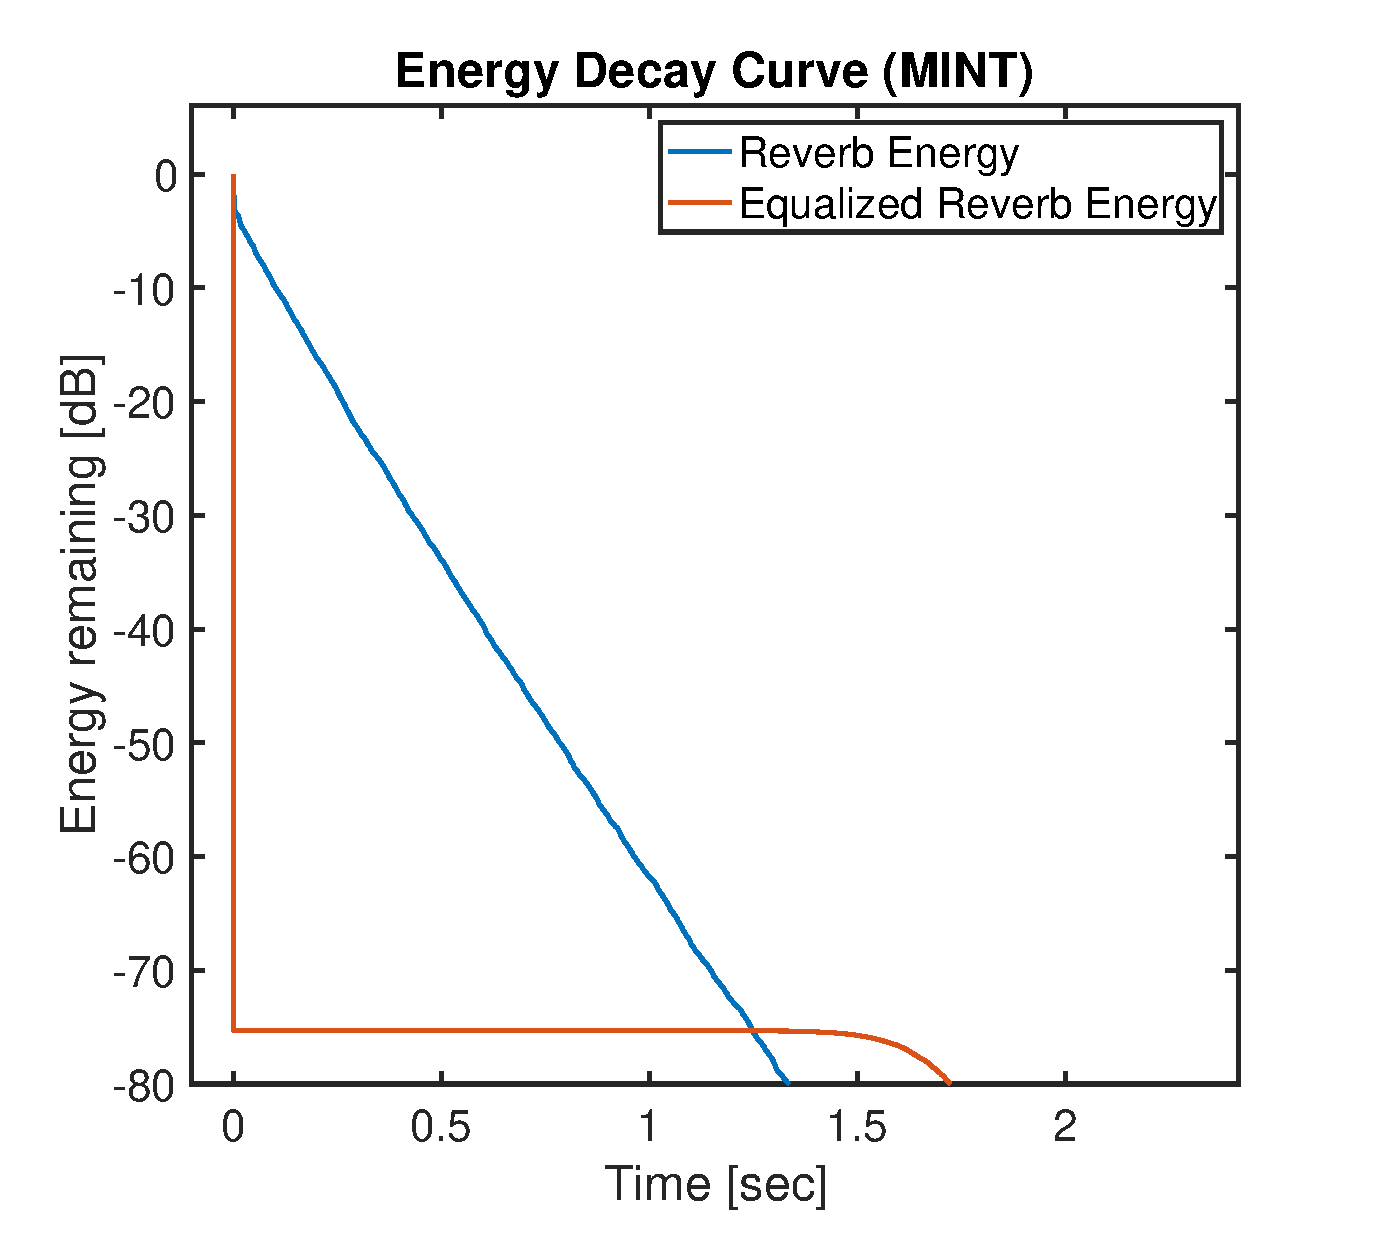
\includegraphics[width=\textwidth]{FullExample_MINT_EDC}
	\end{subfigure}
	\begin{subfigure}[b]{0.49\textwidth}
		\centering
		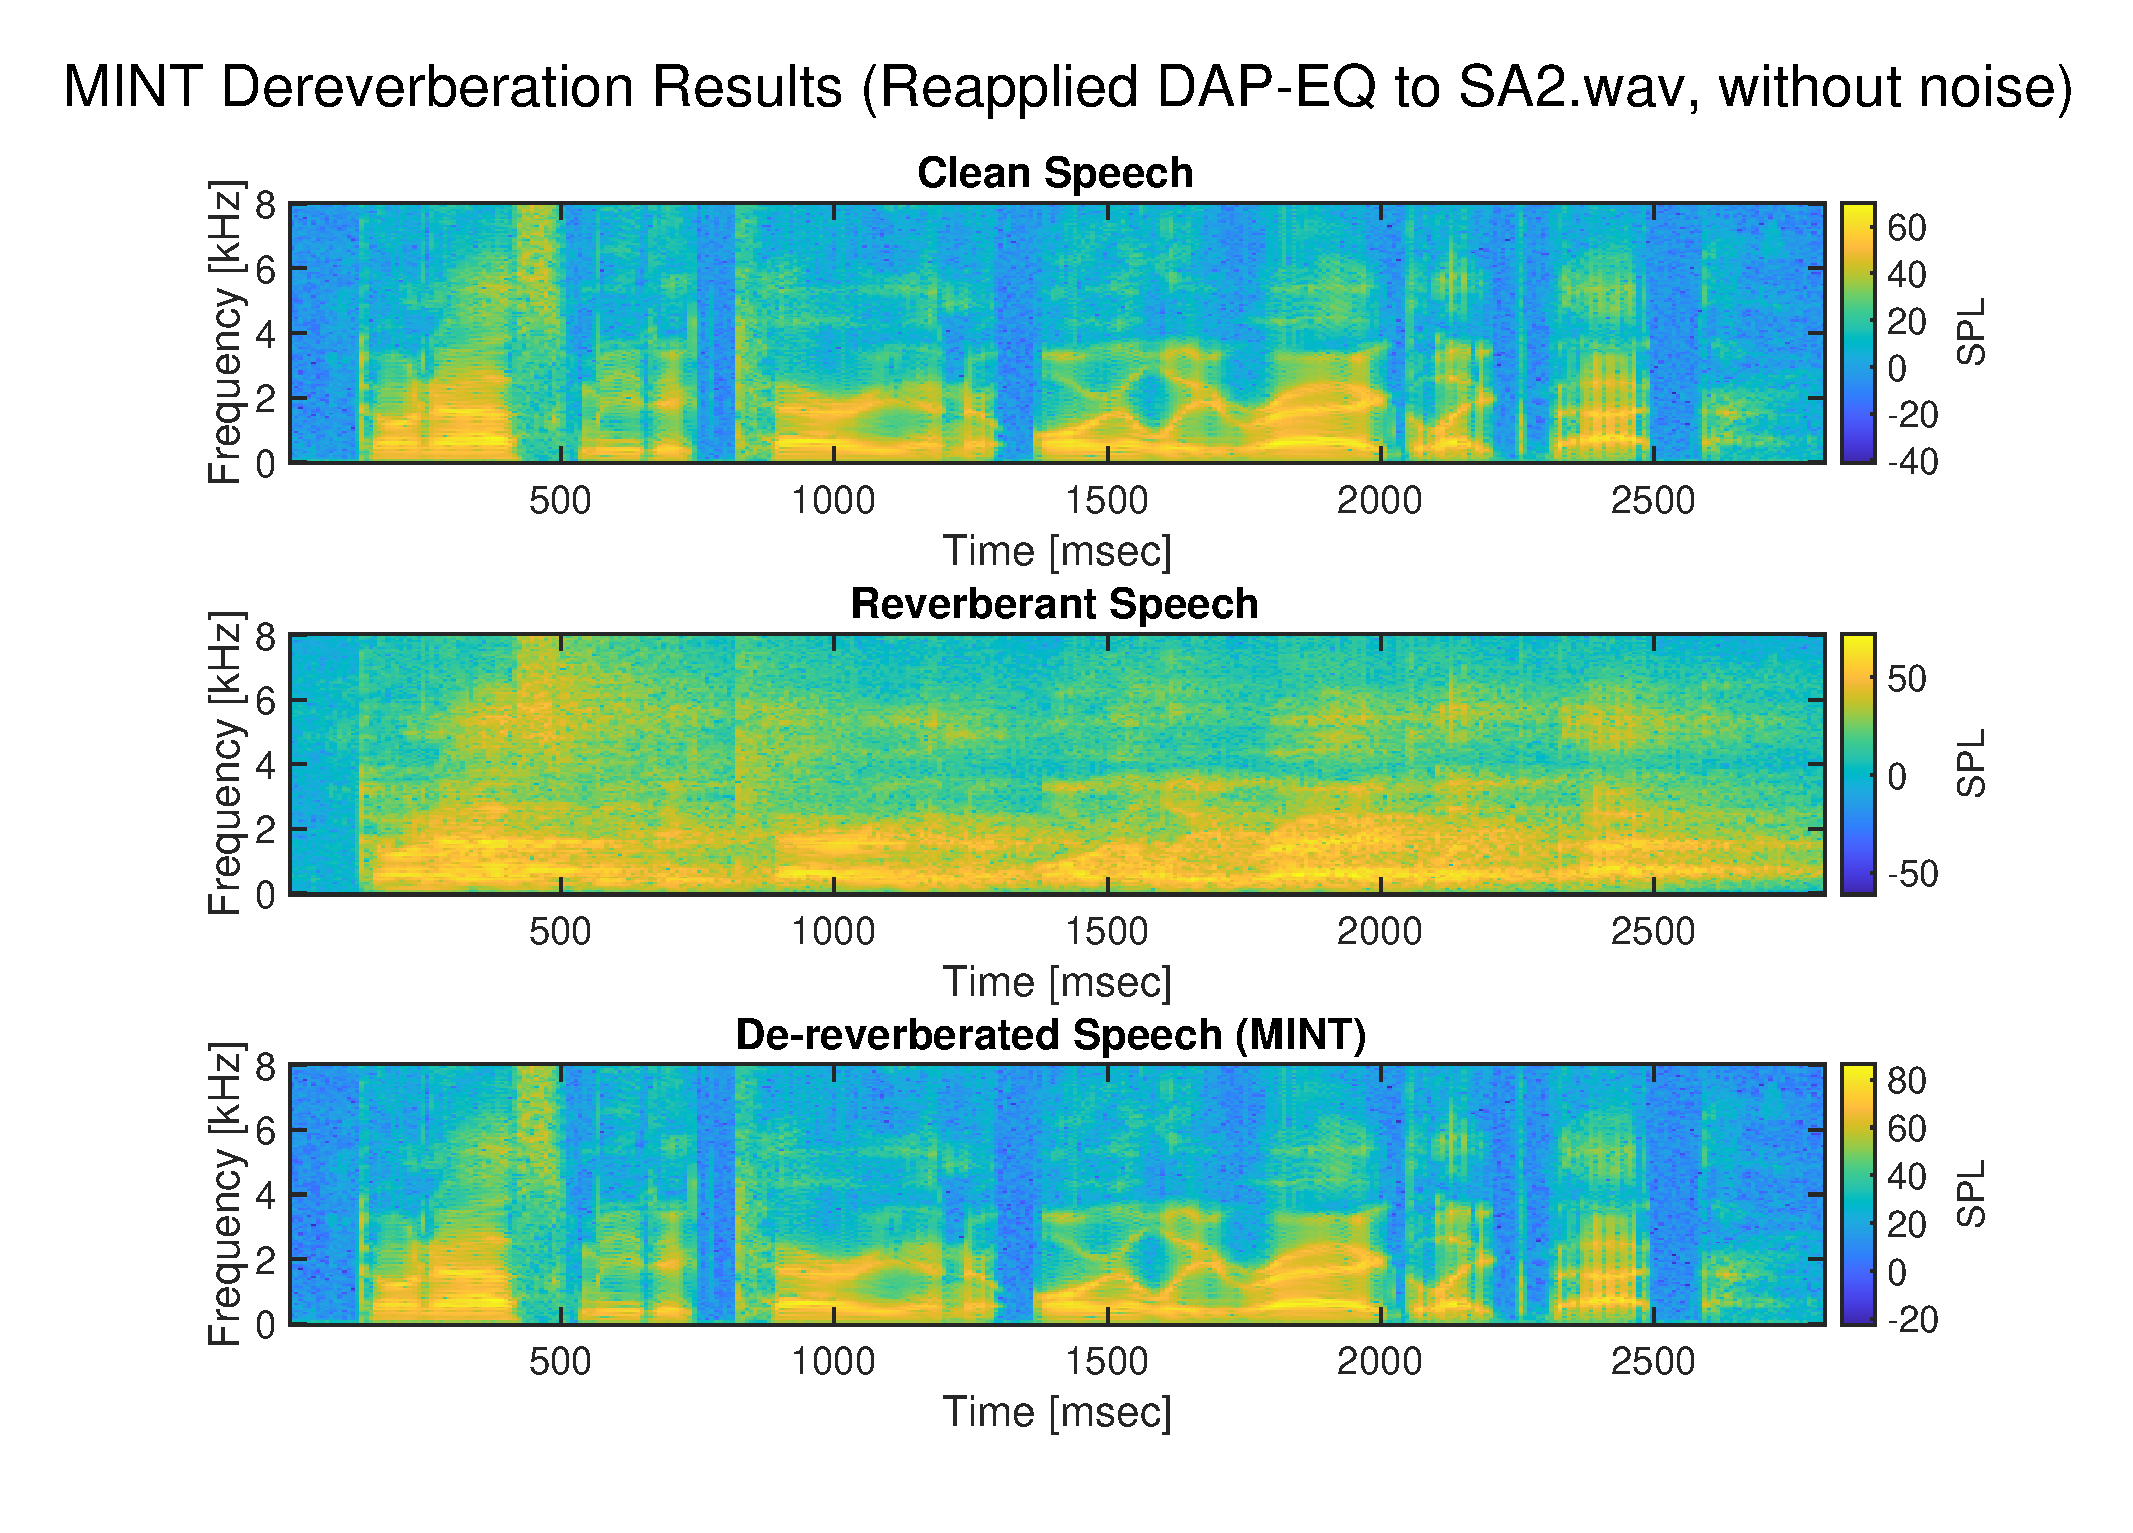
\includegraphics[width=\textwidth]{FullExample_MINT_Spectrogram}
	\end{subfigure}
	\caption{MINT Equalizer performance (EDC and Spectrogram)}
	\label{fig:fullExample_MINT}
\end{figure}


\begin{figure}[H]
	\centering
	\begin{subfigure}[b]{0.38\textwidth}
		\centering
		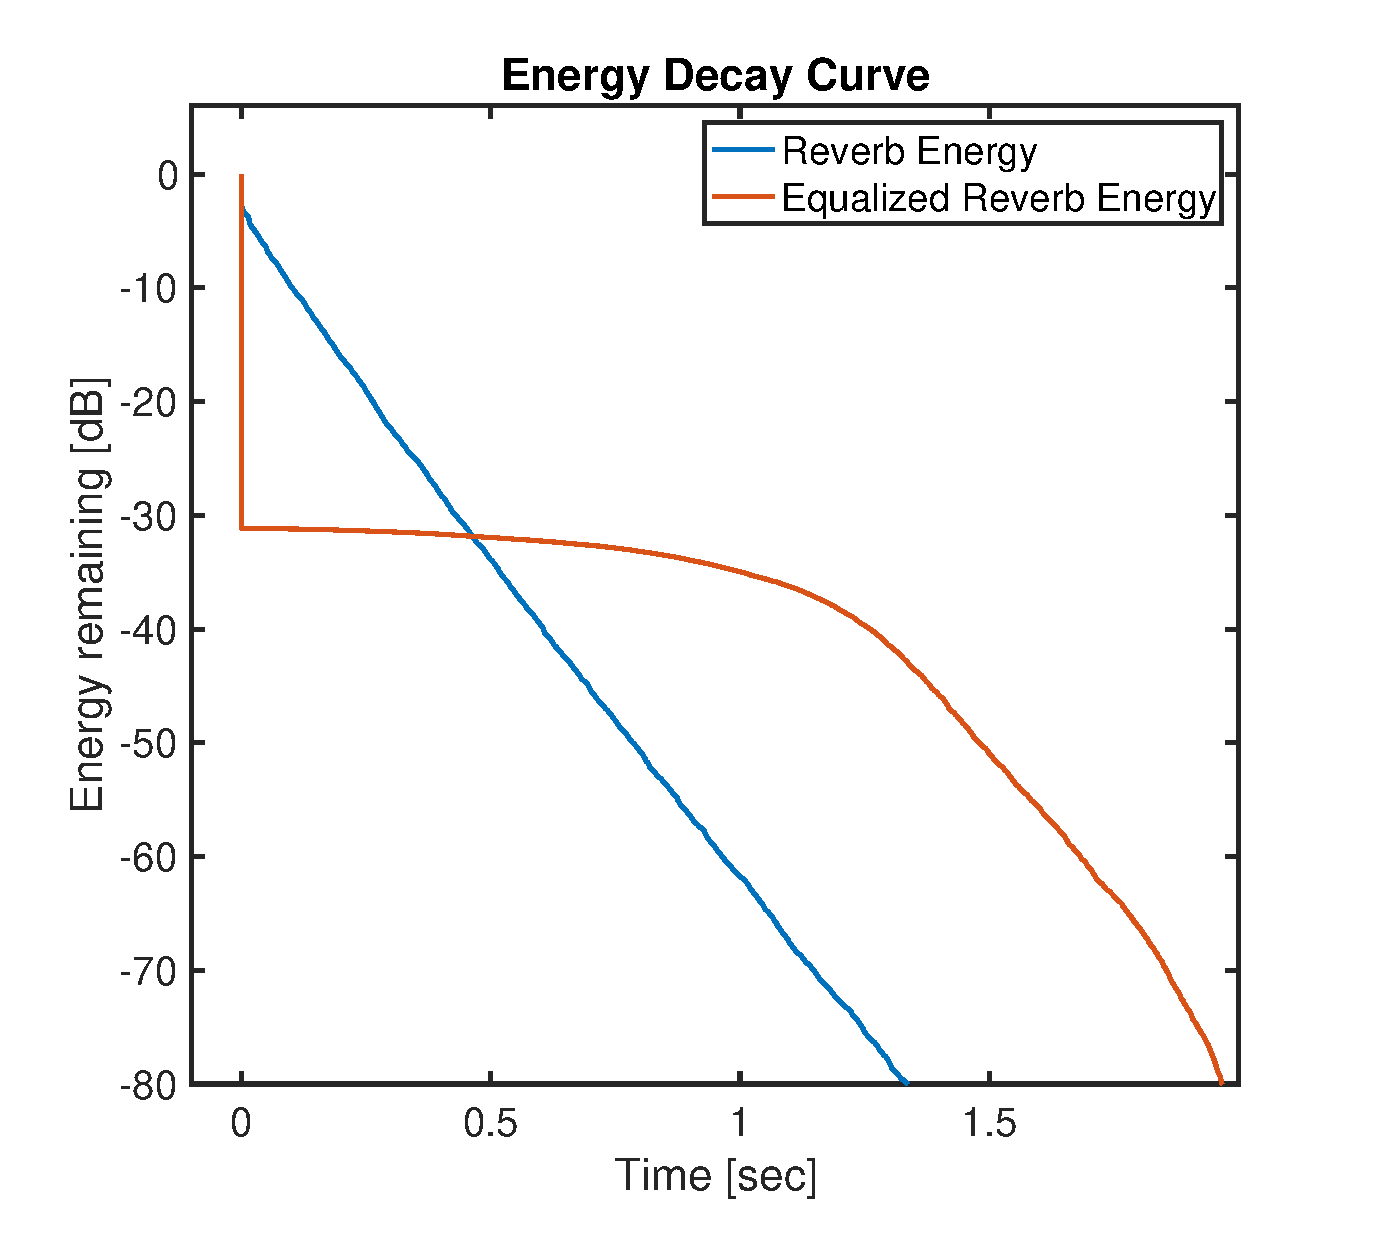
\includegraphics[width=\textwidth]{FullExample_NotBlind_EDC}
	\end{subfigure}
	\begin{subfigure}[b]{0.49\textwidth}
		\centering
		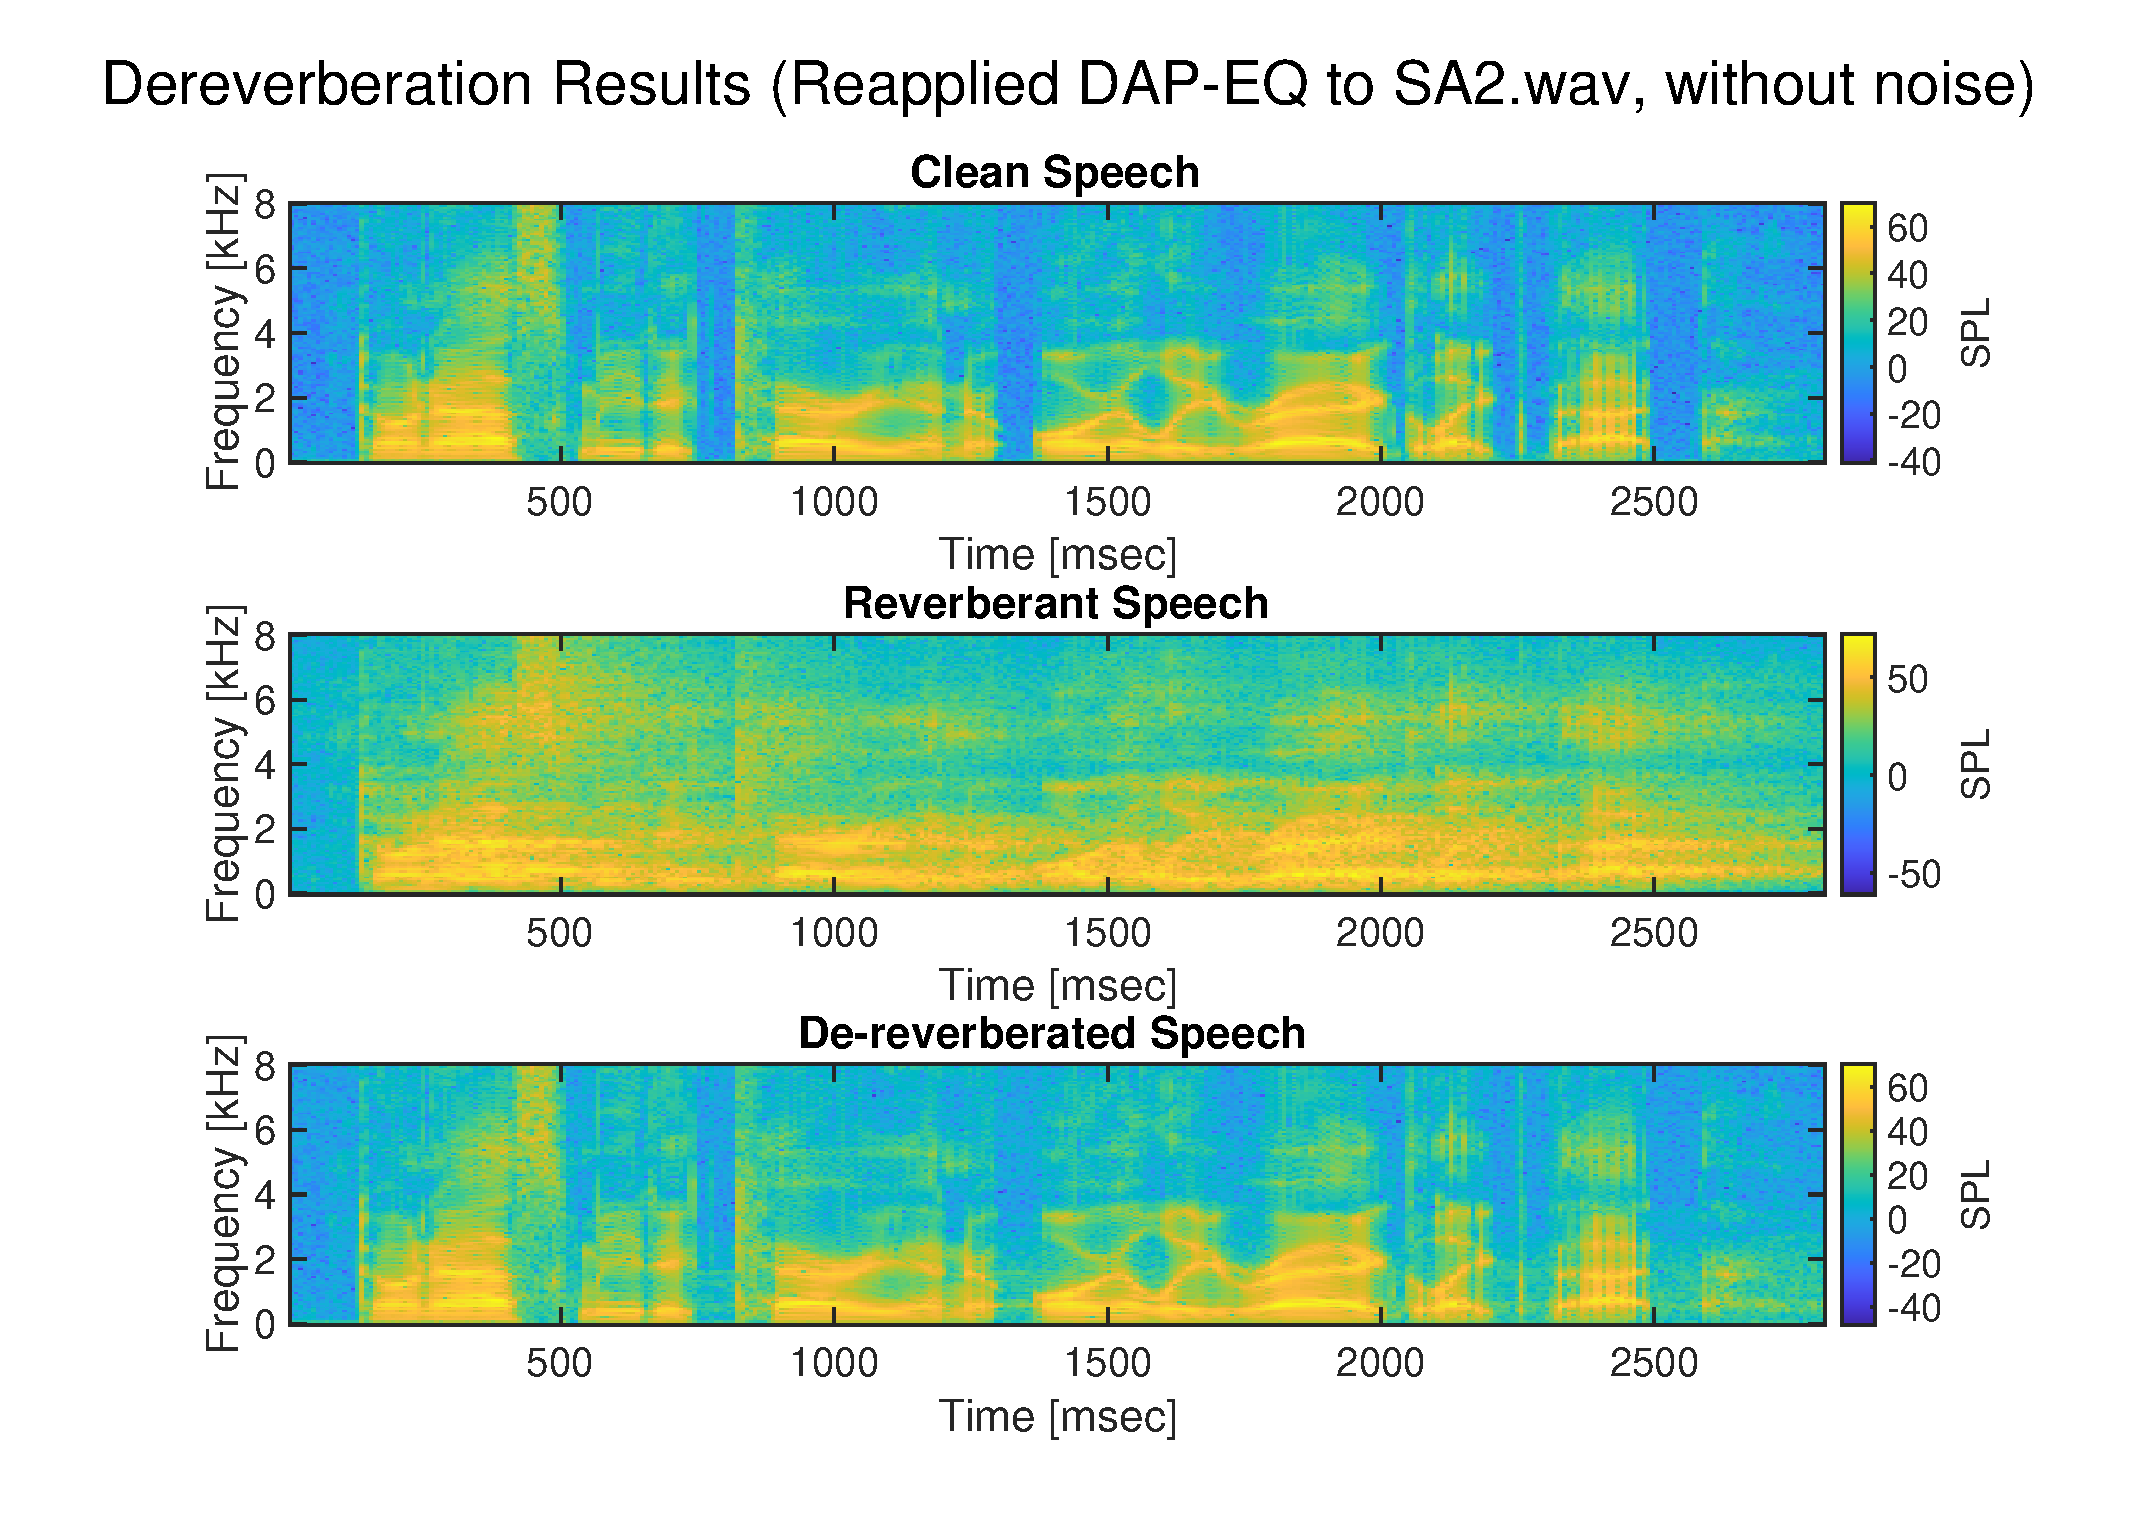
\includegraphics[width=\textwidth]{FullExample_NotBlind_Spectrogram}
	\end{subfigure}
	\caption{Delay-and-Predict Equalizer performance (EDC and Spectrogram) with the source-whitening filter computed using clean speech (i.e., not blind)}
	\label{fig:fullExample_NotBlind}
\end{figure}


\begin{figure}[H]
	\centering
	\begin{subfigure}[b]{0.38\textwidth}
		\centering
		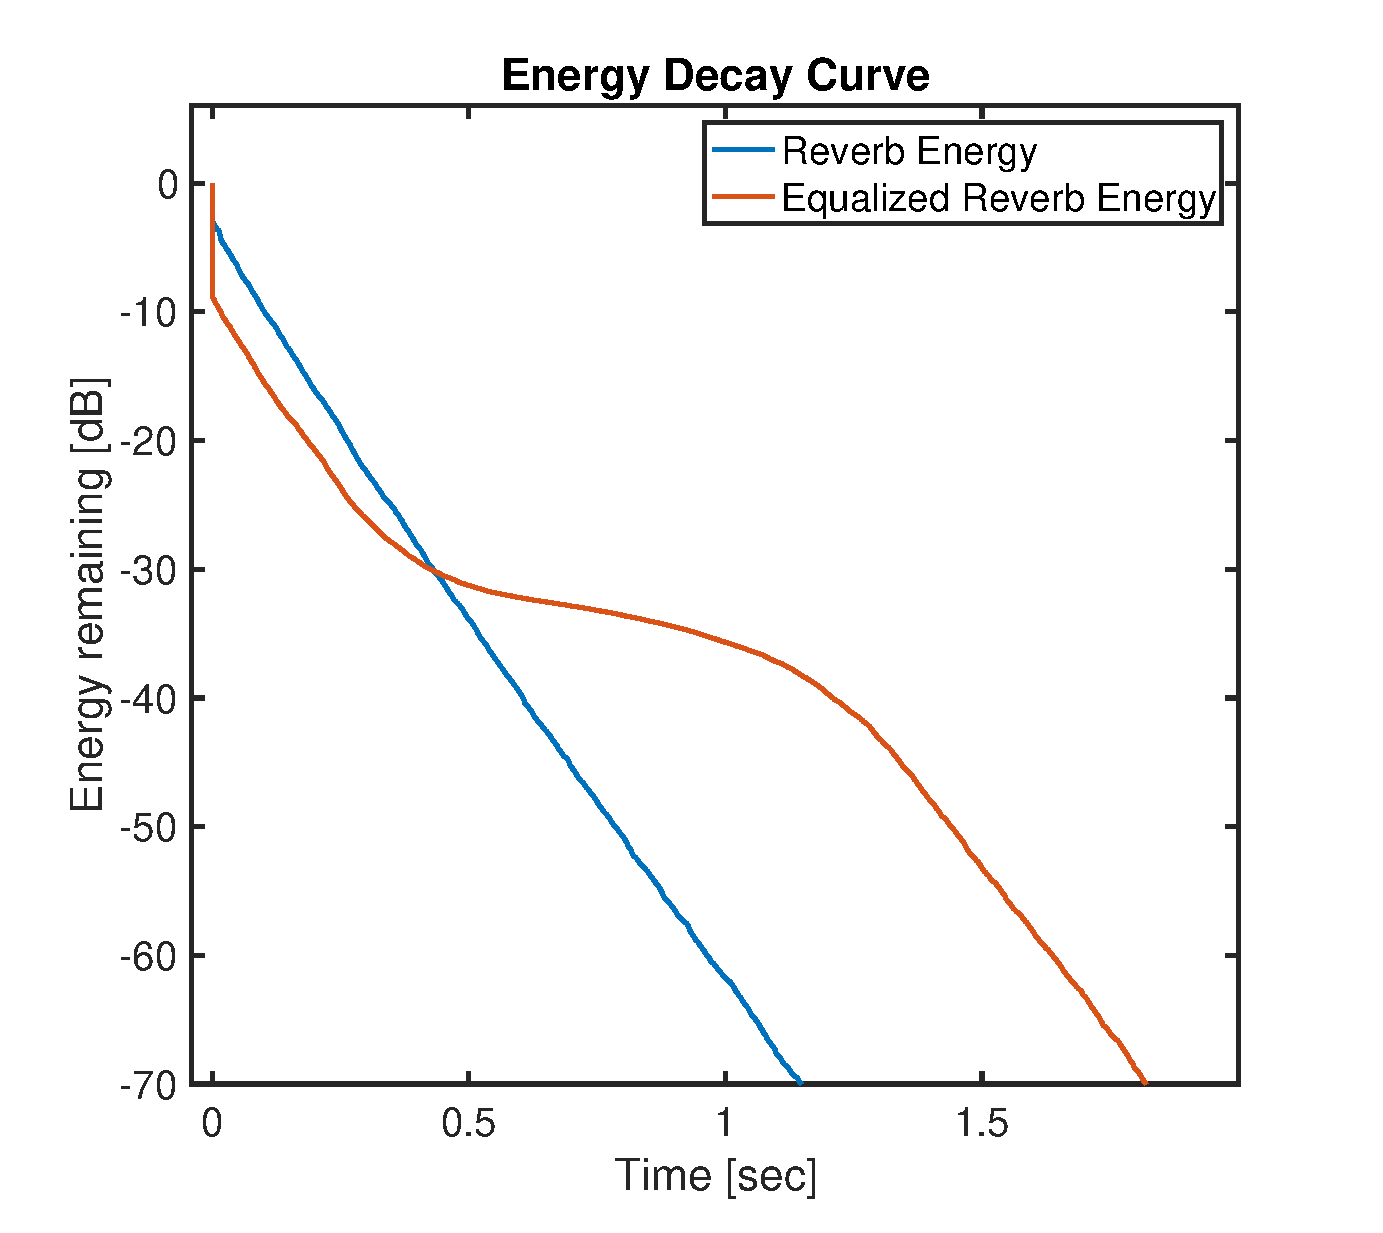
\includegraphics[width=\textwidth]{FullExample_Blind_EDC}
	\end{subfigure}
	\begin{subfigure}[b]{0.49\textwidth}
		\centering
		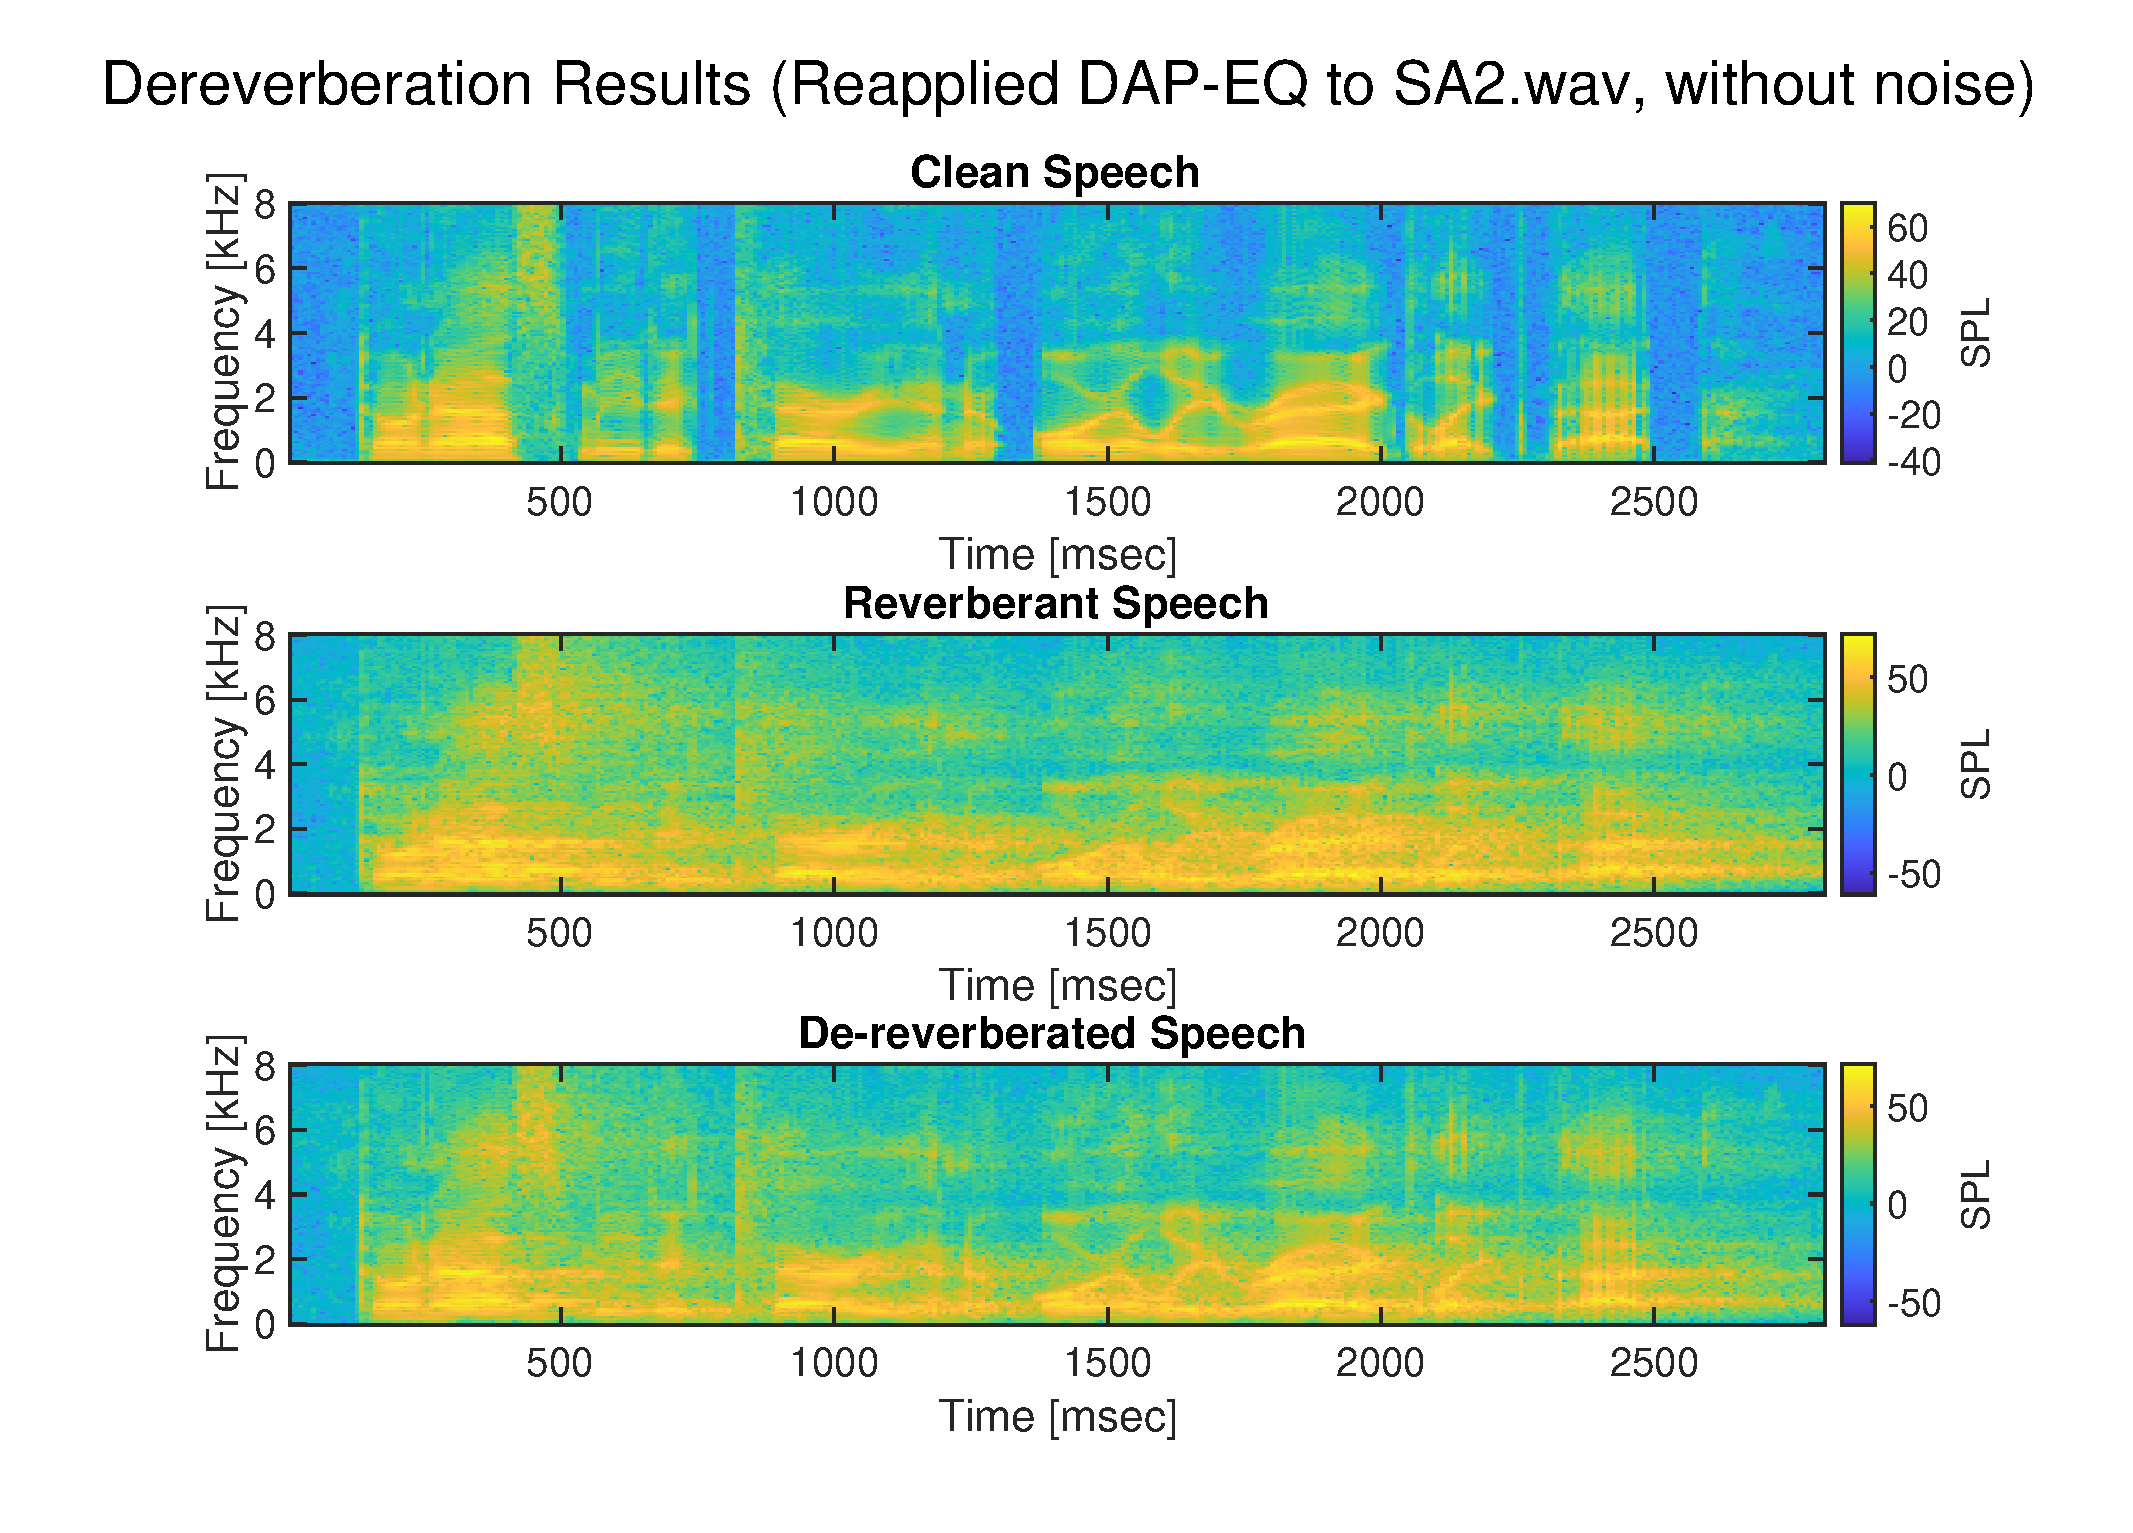
\includegraphics[width=\textwidth]{FullExample_Blind_Spectrogram}
	\end{subfigure}
	\caption{Delay-and-Predict Equalizer performance (EDC and Spectrogram) with the source-whitening filter computed using reverberant speech (i.e., blind)}
	\label{fig:fullExample_Blind}
\end{figure}




\section{Source Properties}


\subsection{Source Data Length}

Test: Same spectrum different length
•	Run 2x with source whitening done on clean (supervised) and revererant signals (blind)
•	Speech is SA1.wav looped X times
•	RIR = SAL truncated to 100 msec = 1600 samples, M = 4 mics
•	P1 = 2 * p2 * (M-1)
•	P2 = N60 / (M-1)
•	Reran exact same test for longer source sequences generated by looping SA1 – Exact same spectrum just more data (excludes spectrum dependency)

\textbf{Source Data Length Compare, Length = [58061  116122 174183 232244 ], Blind}

\begin{figure}[H]
	\centering
	\begin{subfigure}[b]{0.3\textwidth}
		\centering
		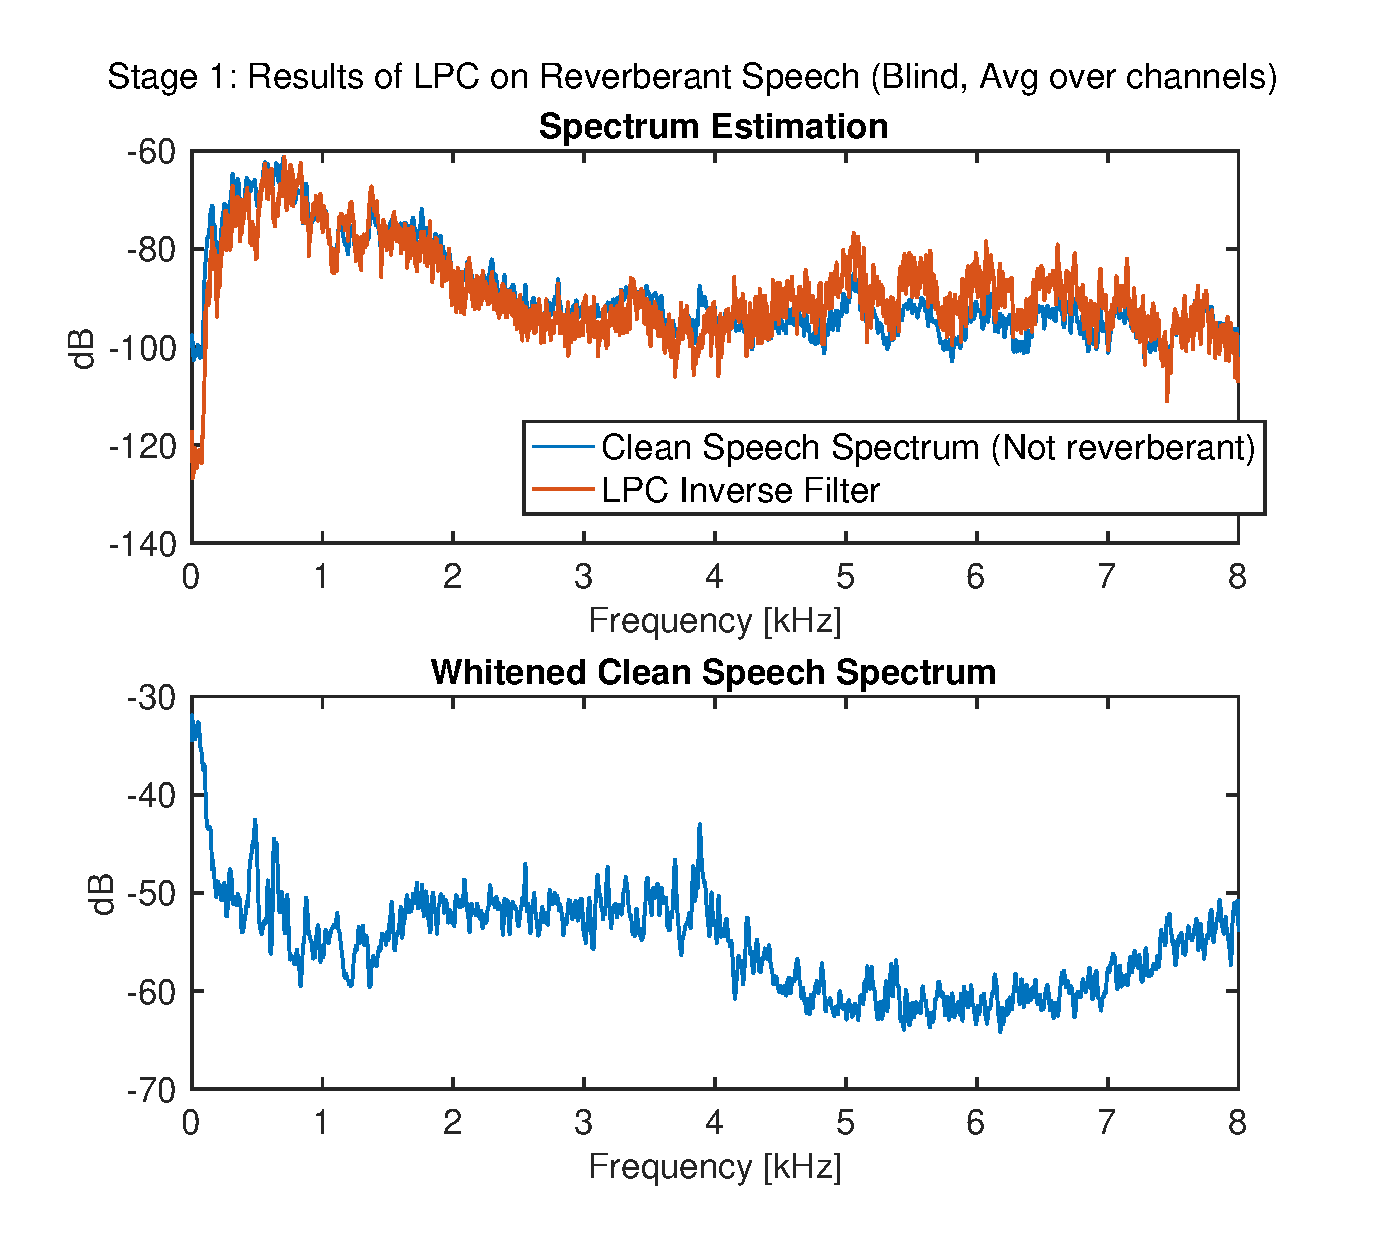
\includegraphics[width=\textwidth]{S1_SourceLength_1_Blind}
	\end{subfigure}
	\begin{subfigure}[b]{0.3\textwidth}
		\centering
		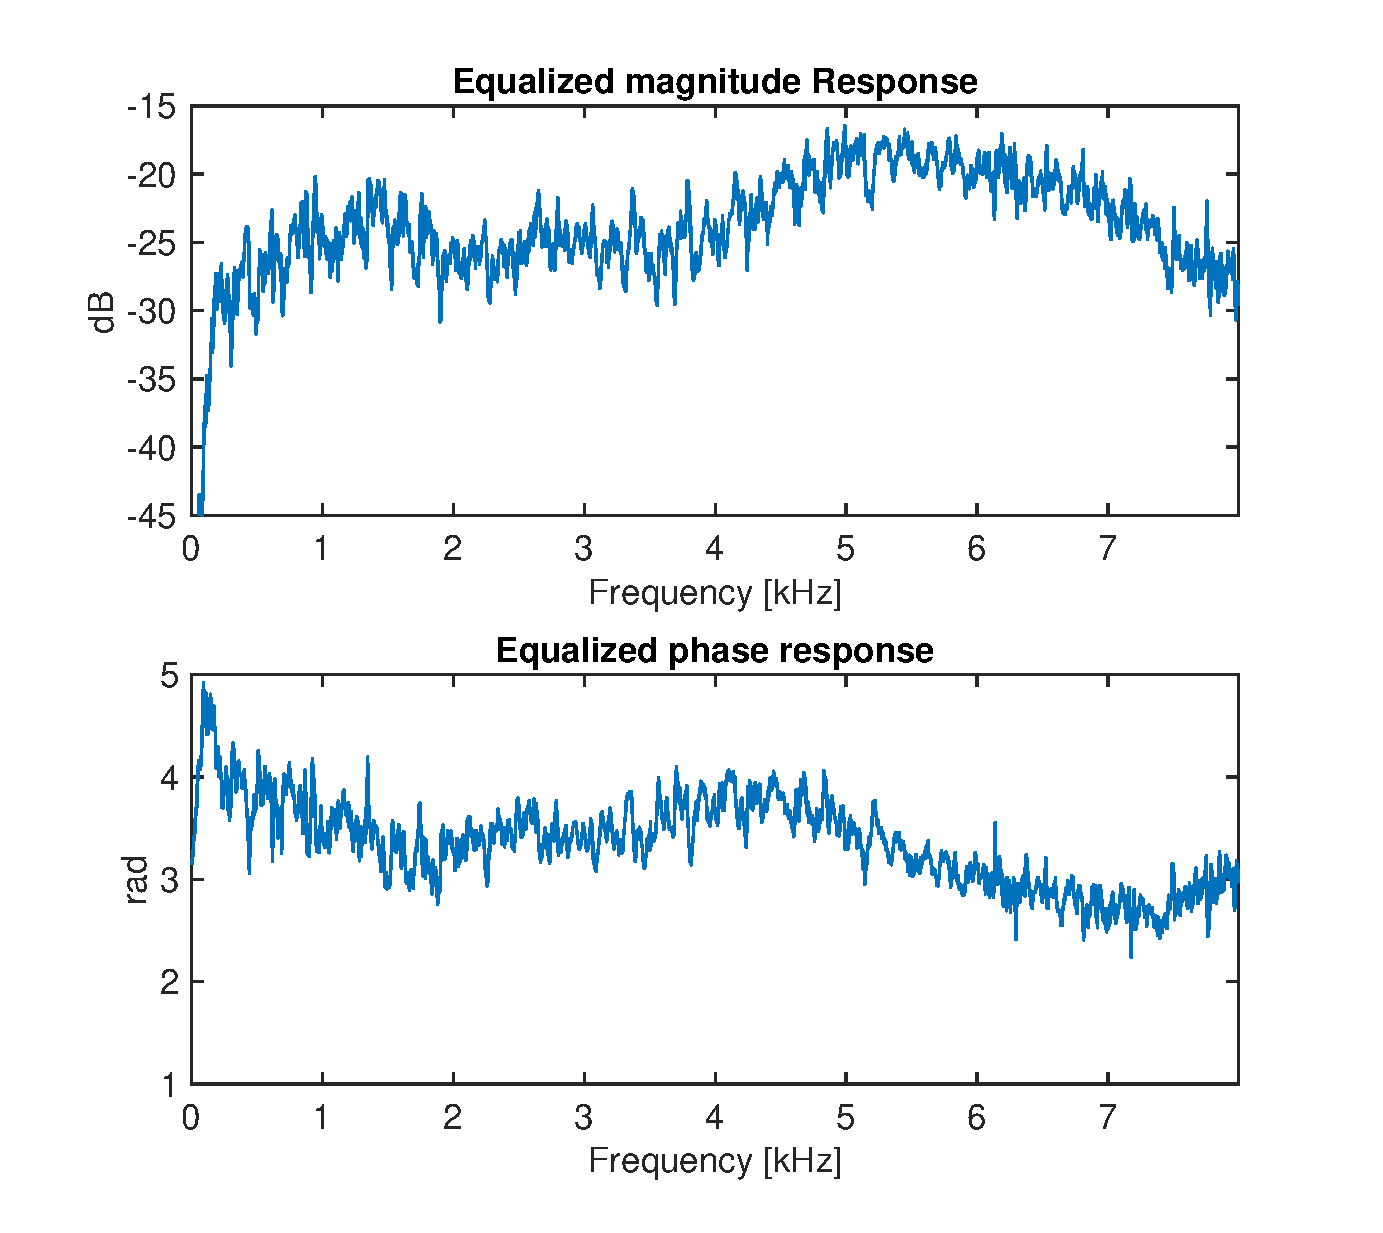
\includegraphics[width=\textwidth]{Equalized_RTF_SourceLength_1_Blind}
	\end{subfigure}
	\begin{subfigure}[b]{0.3\textwidth}
		\centering
		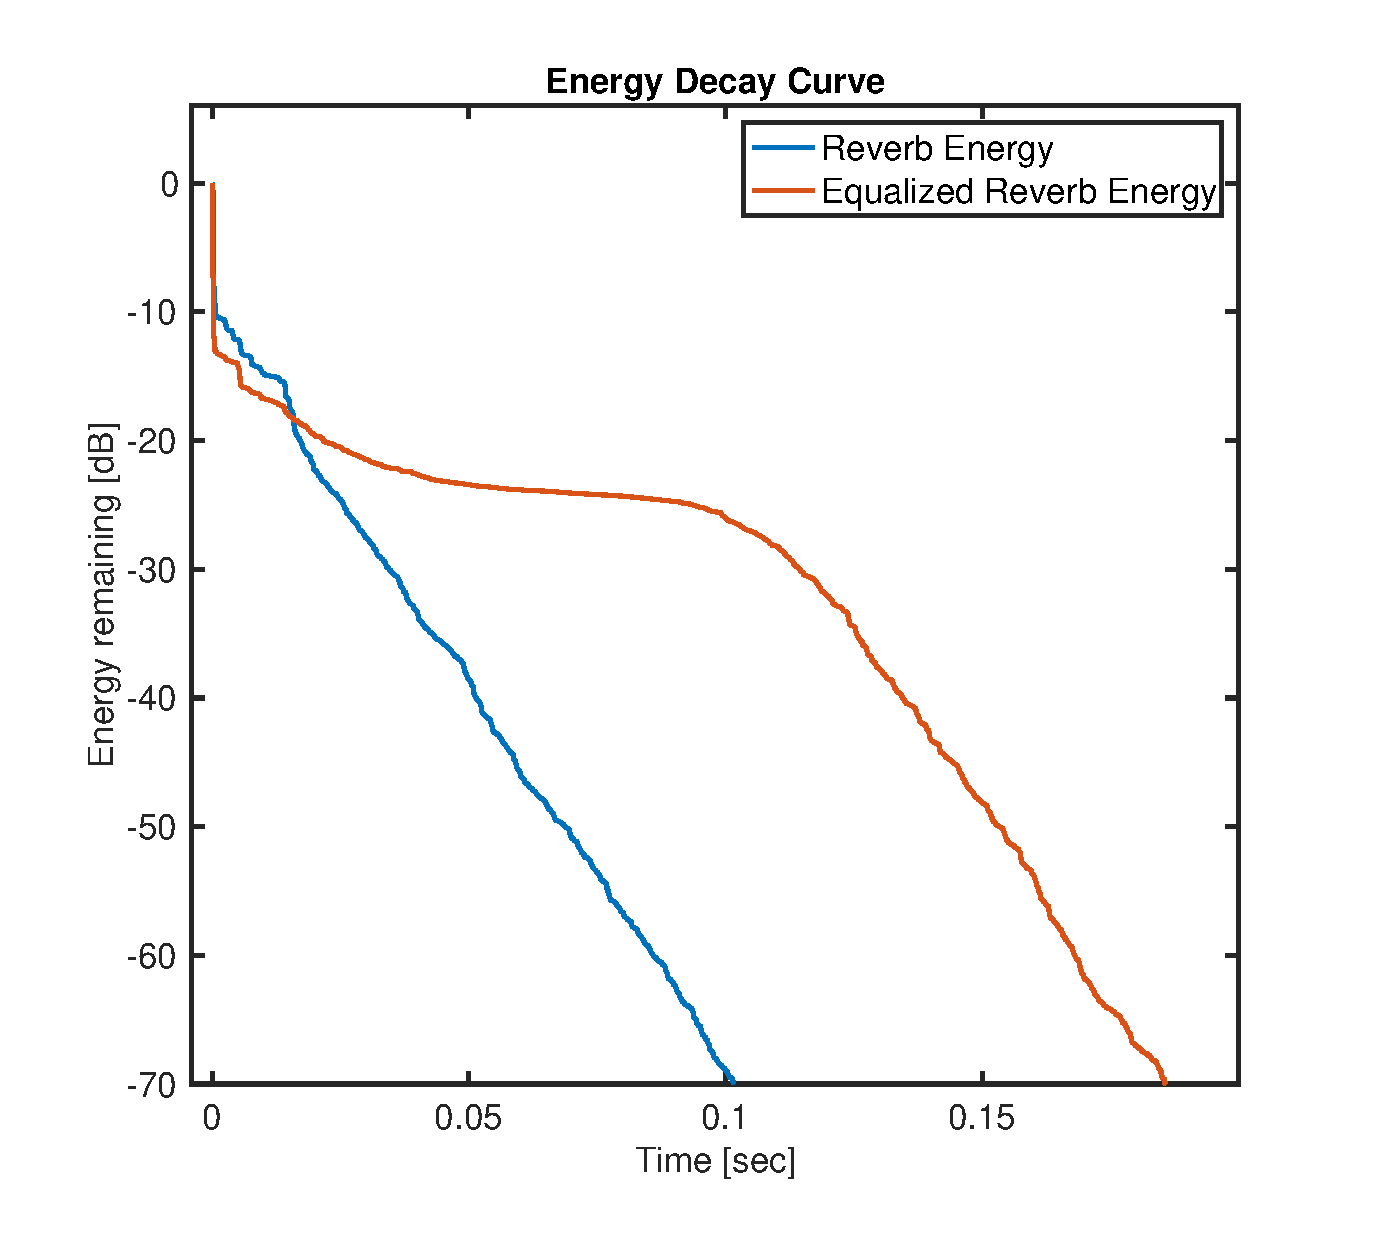
\includegraphics[width=\textwidth]{EDC_SourceLength_1_Blind}
	\end{subfigure}
	\begin{subfigure}[b]{0.3\textwidth}
		\centering
		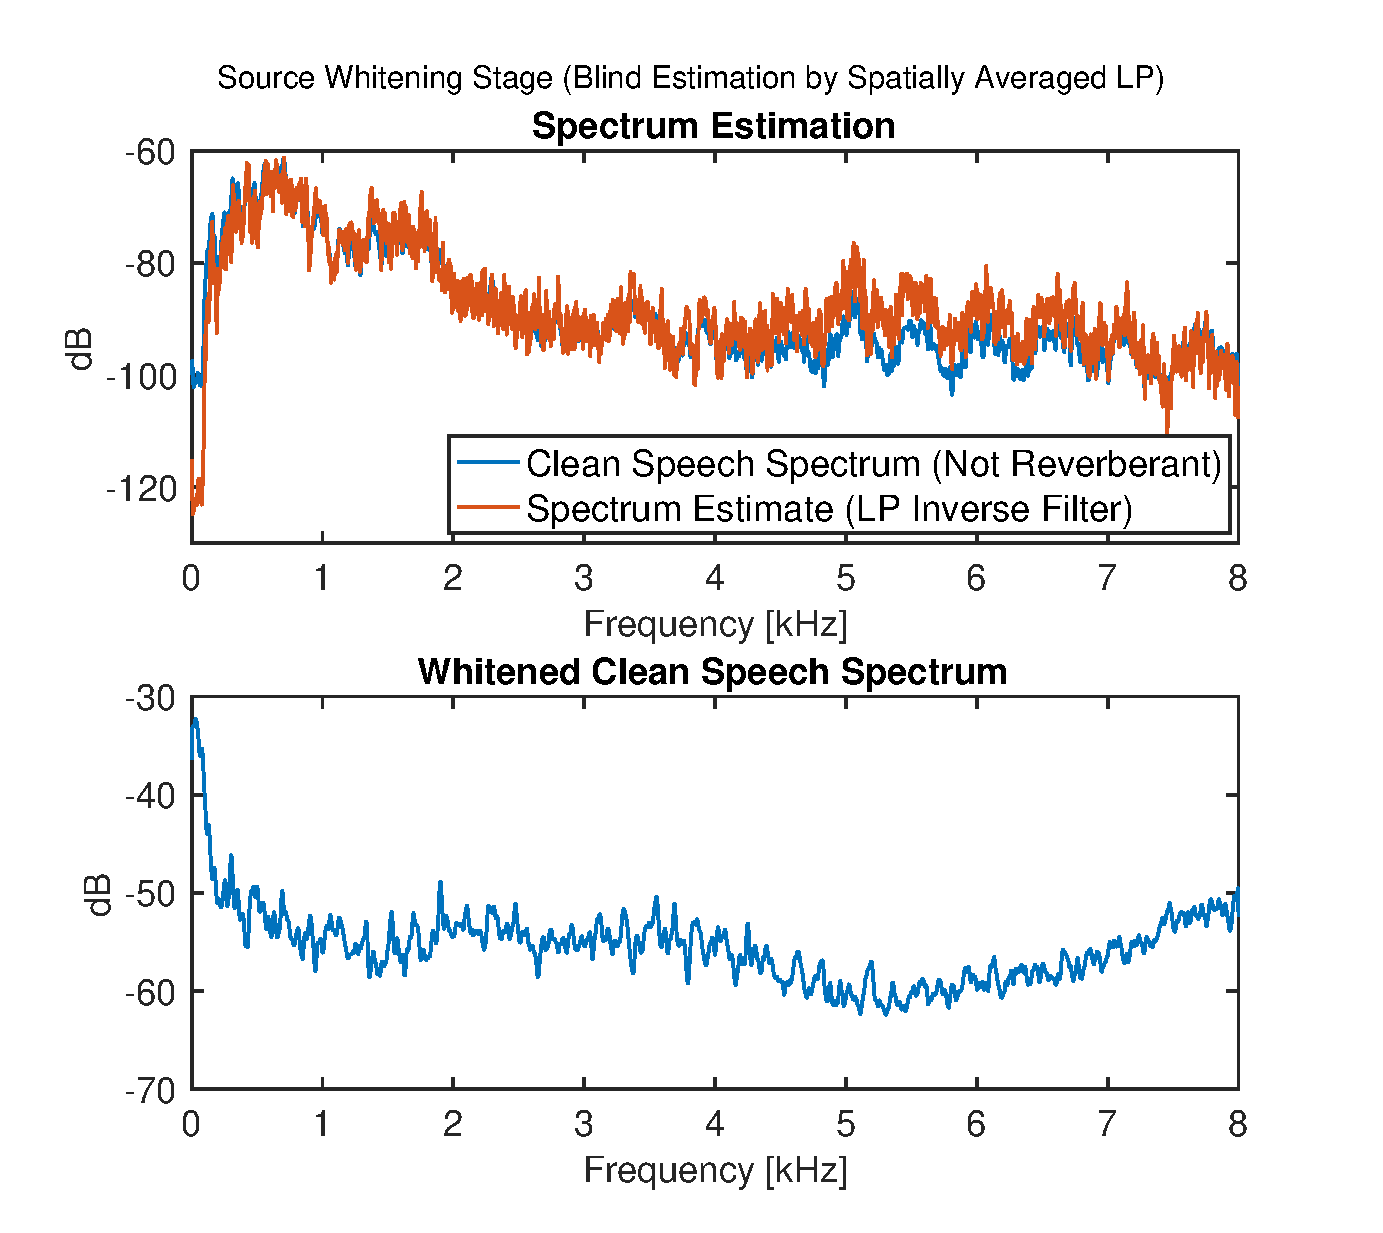
\includegraphics[width=\textwidth]{S1_SourceLength_2_Blind}
	\end{subfigure}
	\begin{subfigure}[b]{0.3\textwidth}
		\centering
		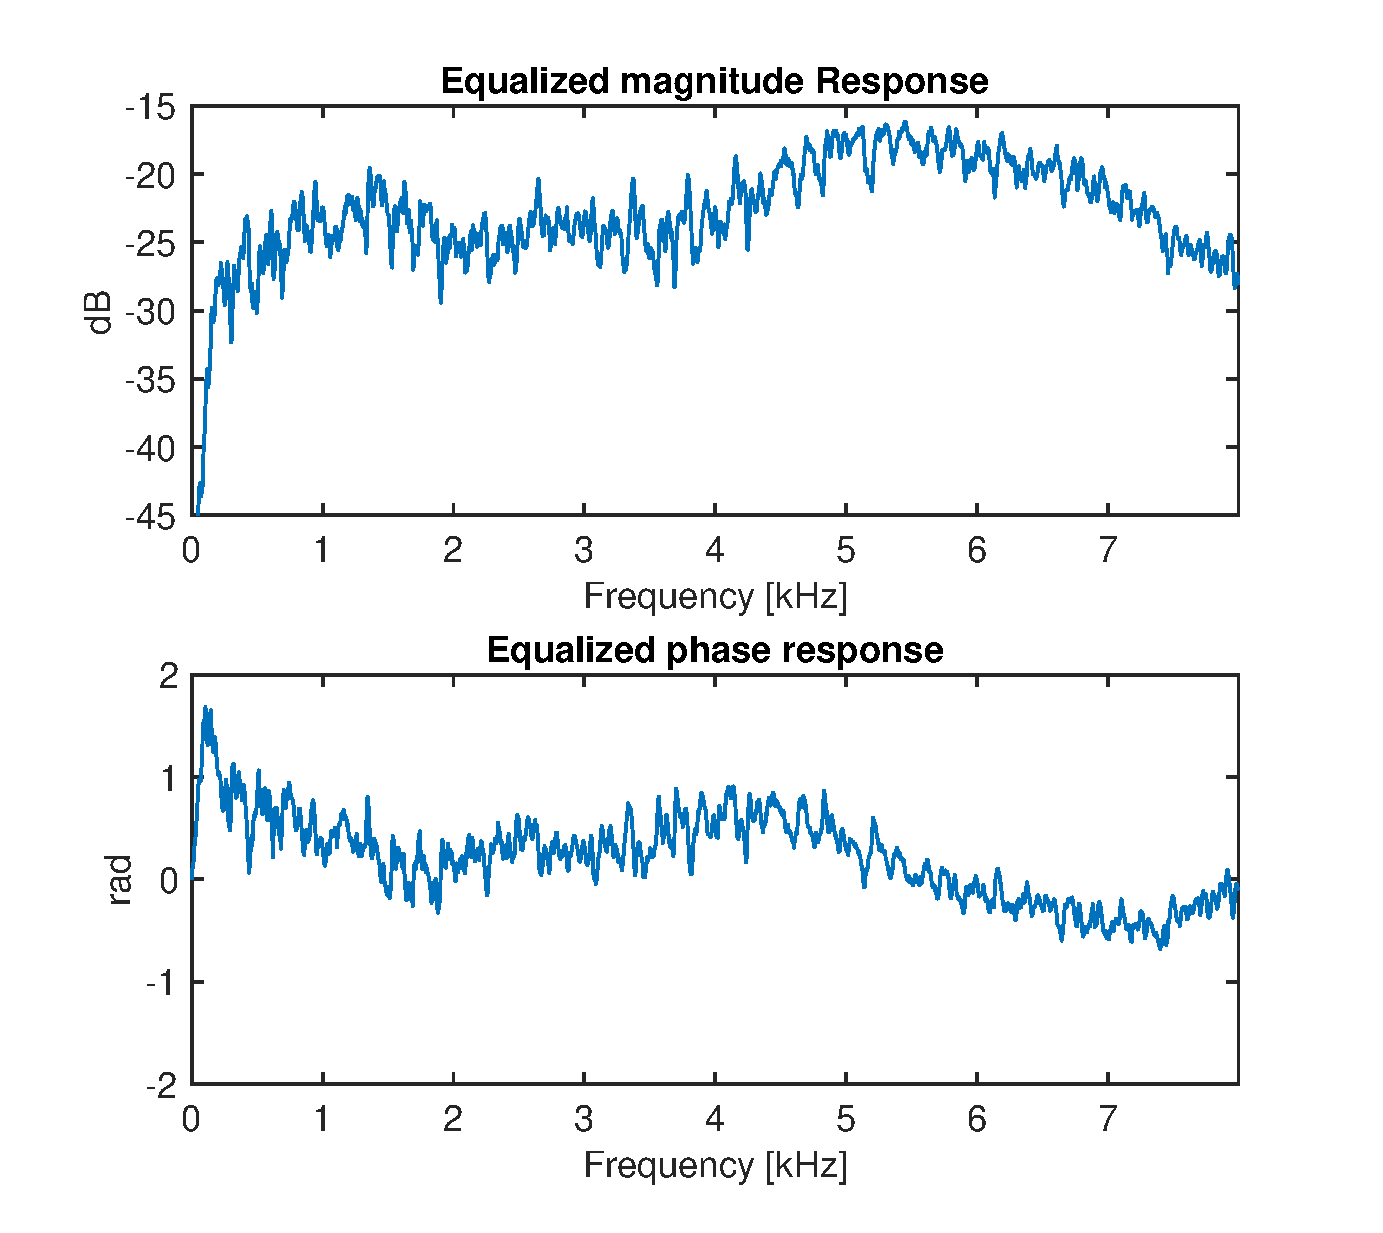
\includegraphics[width=\textwidth]{Equalized_RTF_SourceLength_2_Blind}
	\end{subfigure}
	\begin{subfigure}[b]{0.3\textwidth}
		\centering
		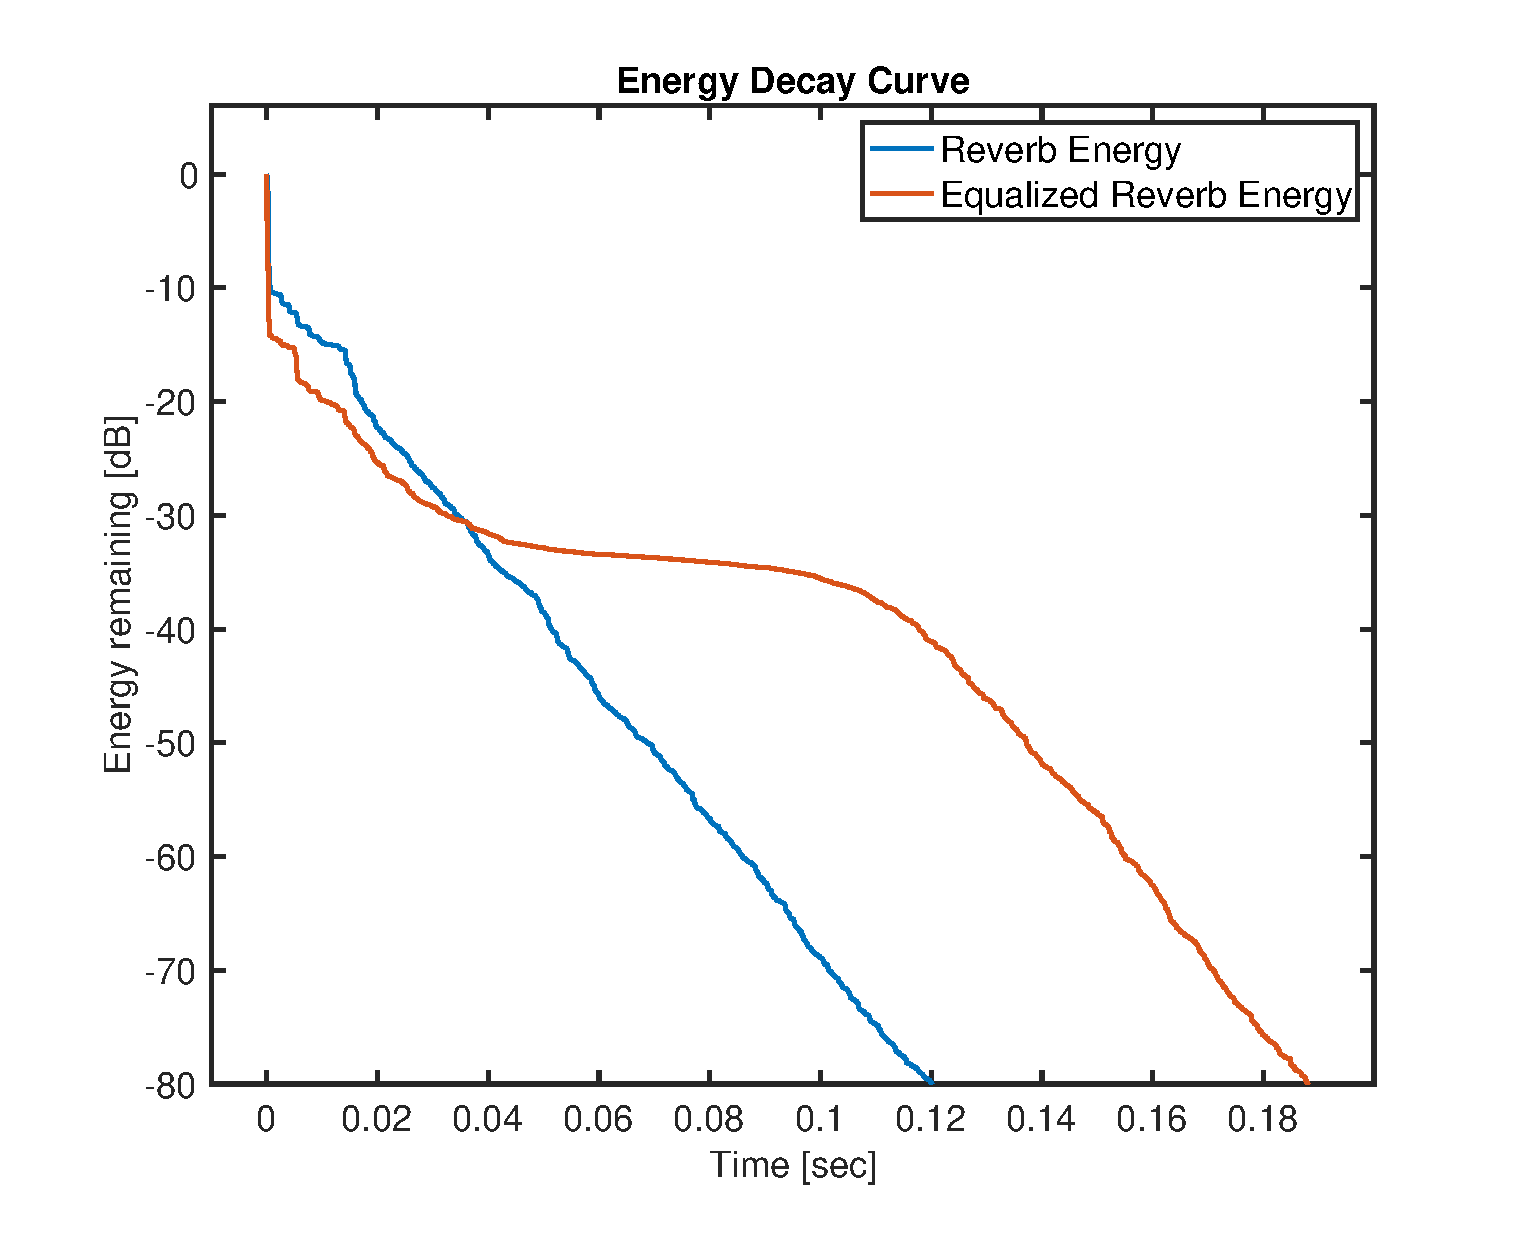
\includegraphics[width=\textwidth]{EDC_SourceLength_2_Blind}
	\end{subfigure}
	\begin{subfigure}[b]{0.3\textwidth}
		\centering
		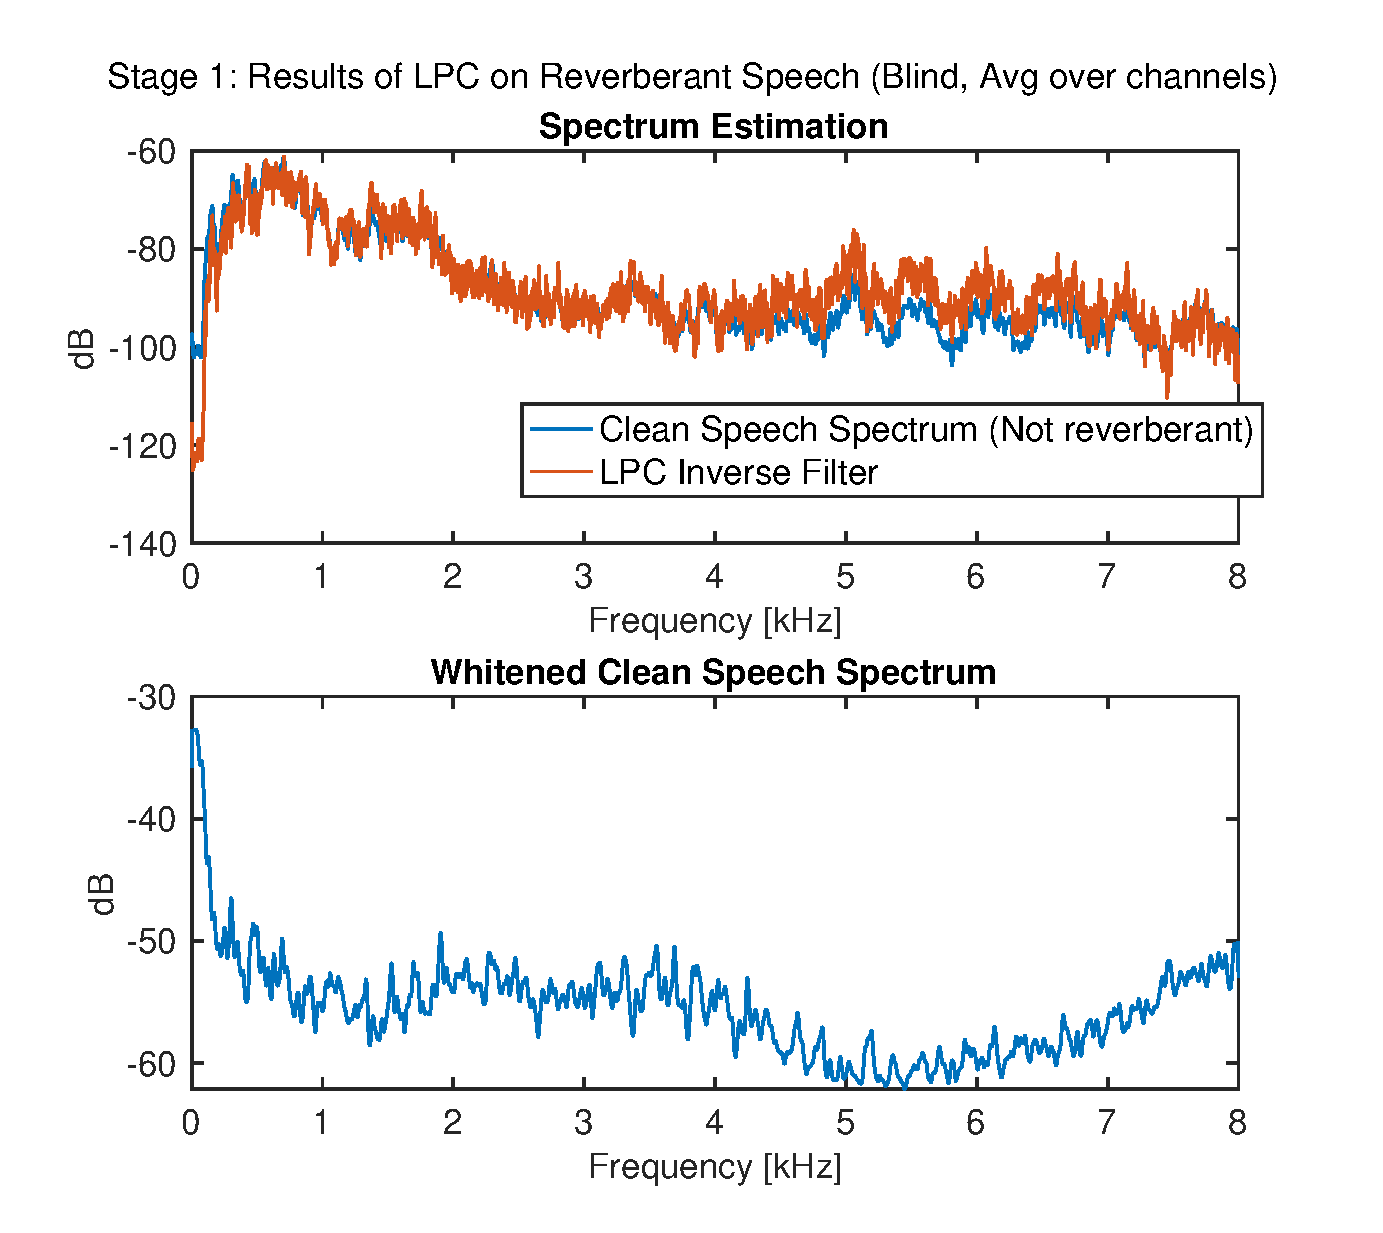
\includegraphics[width=\textwidth]{S1_SourceLength_3_Blind}
	\end{subfigure}
	\begin{subfigure}[b]{0.3\textwidth}
		\centering
		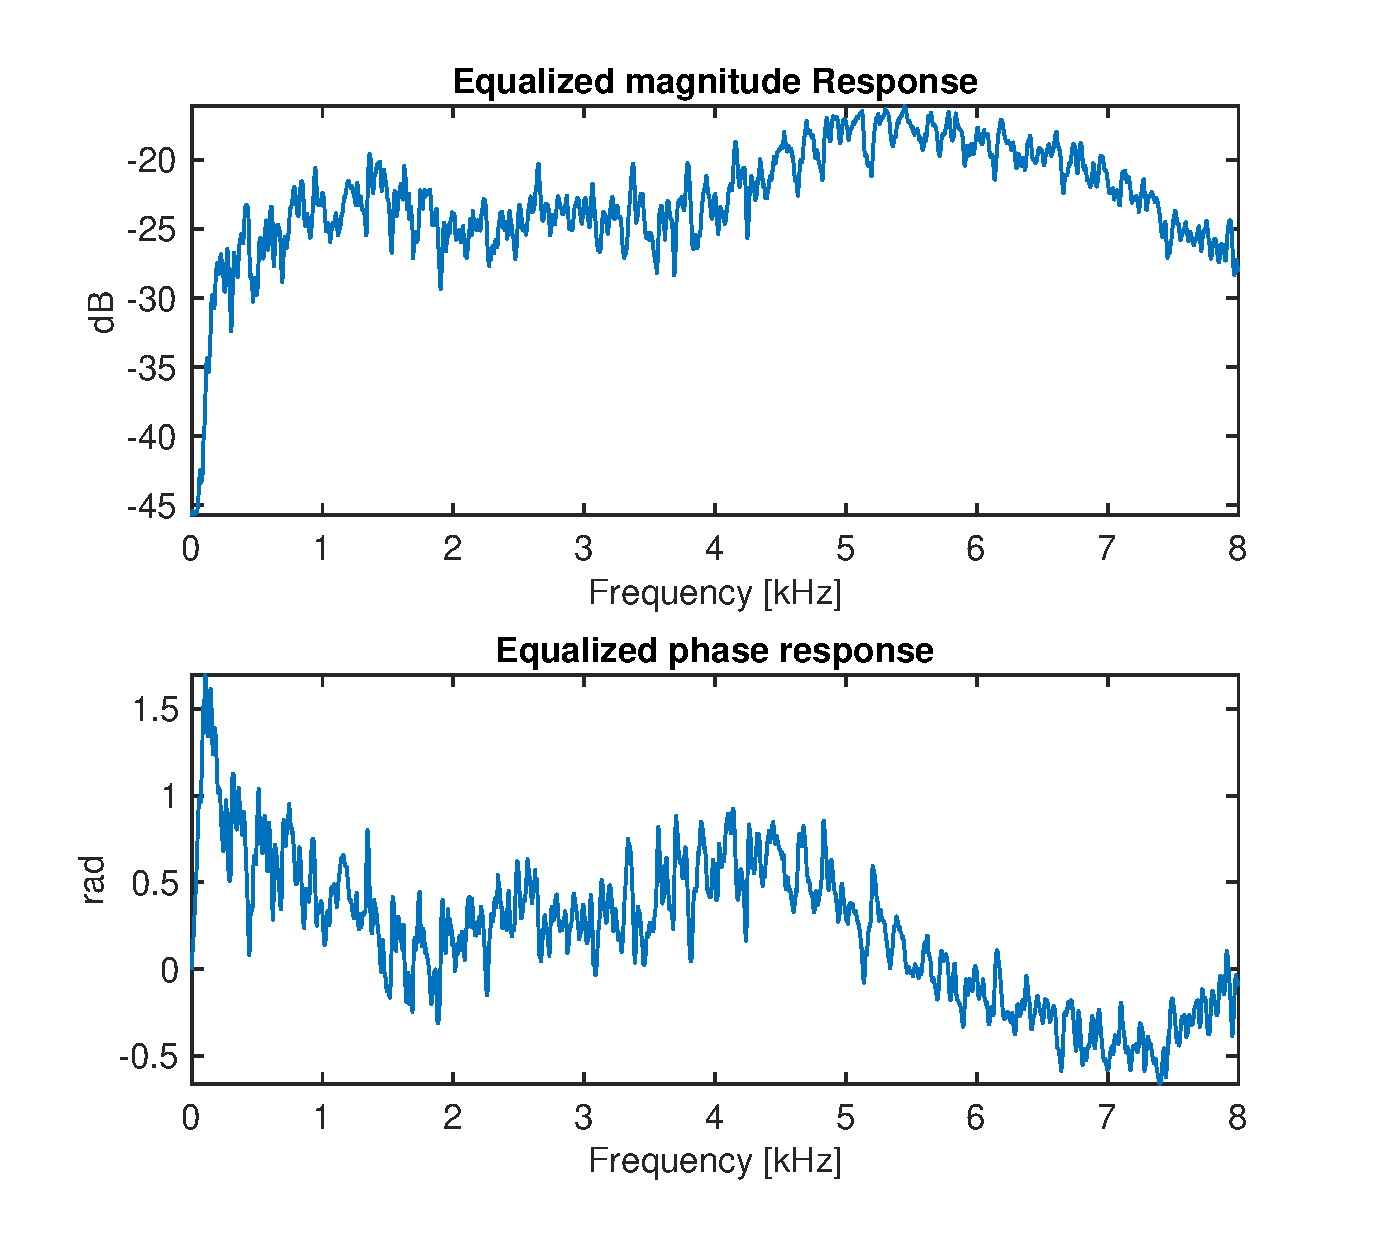
\includegraphics[width=\textwidth]{Equalized_RTF_SourceLength_3_Blind}
	\end{subfigure}
	\begin{subfigure}[b]{0.3\textwidth}
		\centering
		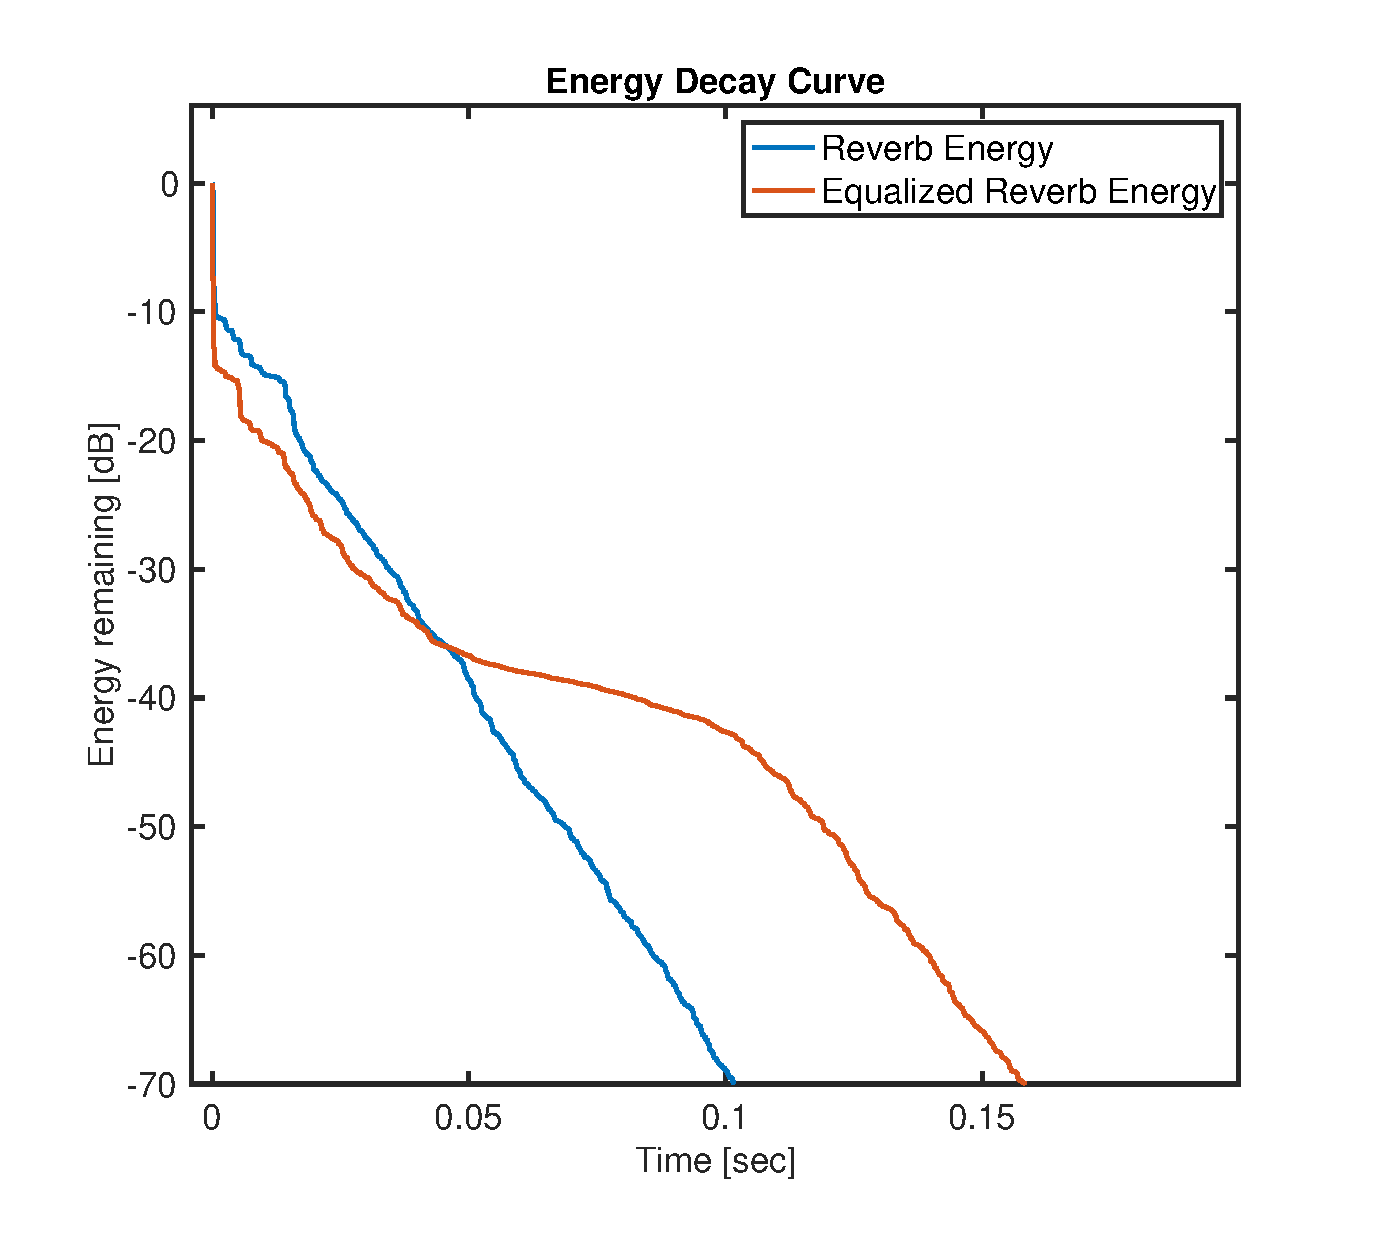
\includegraphics[width=\textwidth]{EDC_SourceLength_3_Blind}
	\end{subfigure}
	\begin{subfigure}[b]{0.3\textwidth}
		\centering
		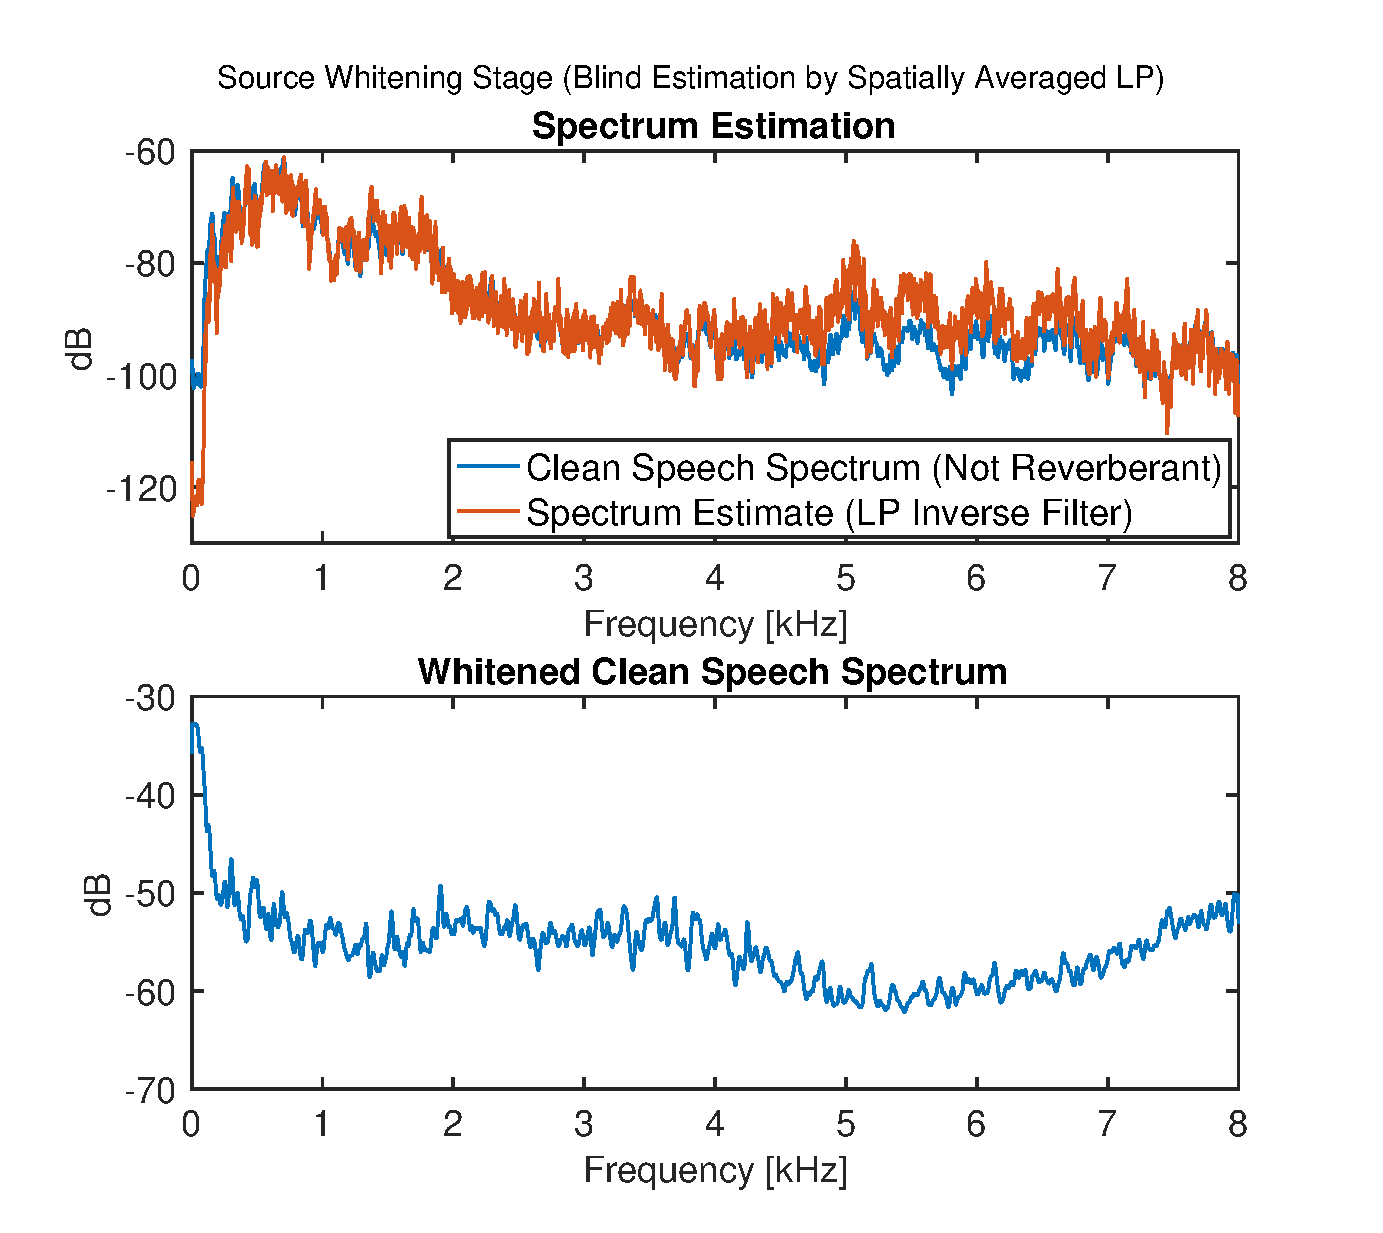
\includegraphics[width=\textwidth]{S1_SourceLength_4_Blind}
	\end{subfigure}
	\begin{subfigure}[b]{0.3\textwidth}
		\centering
		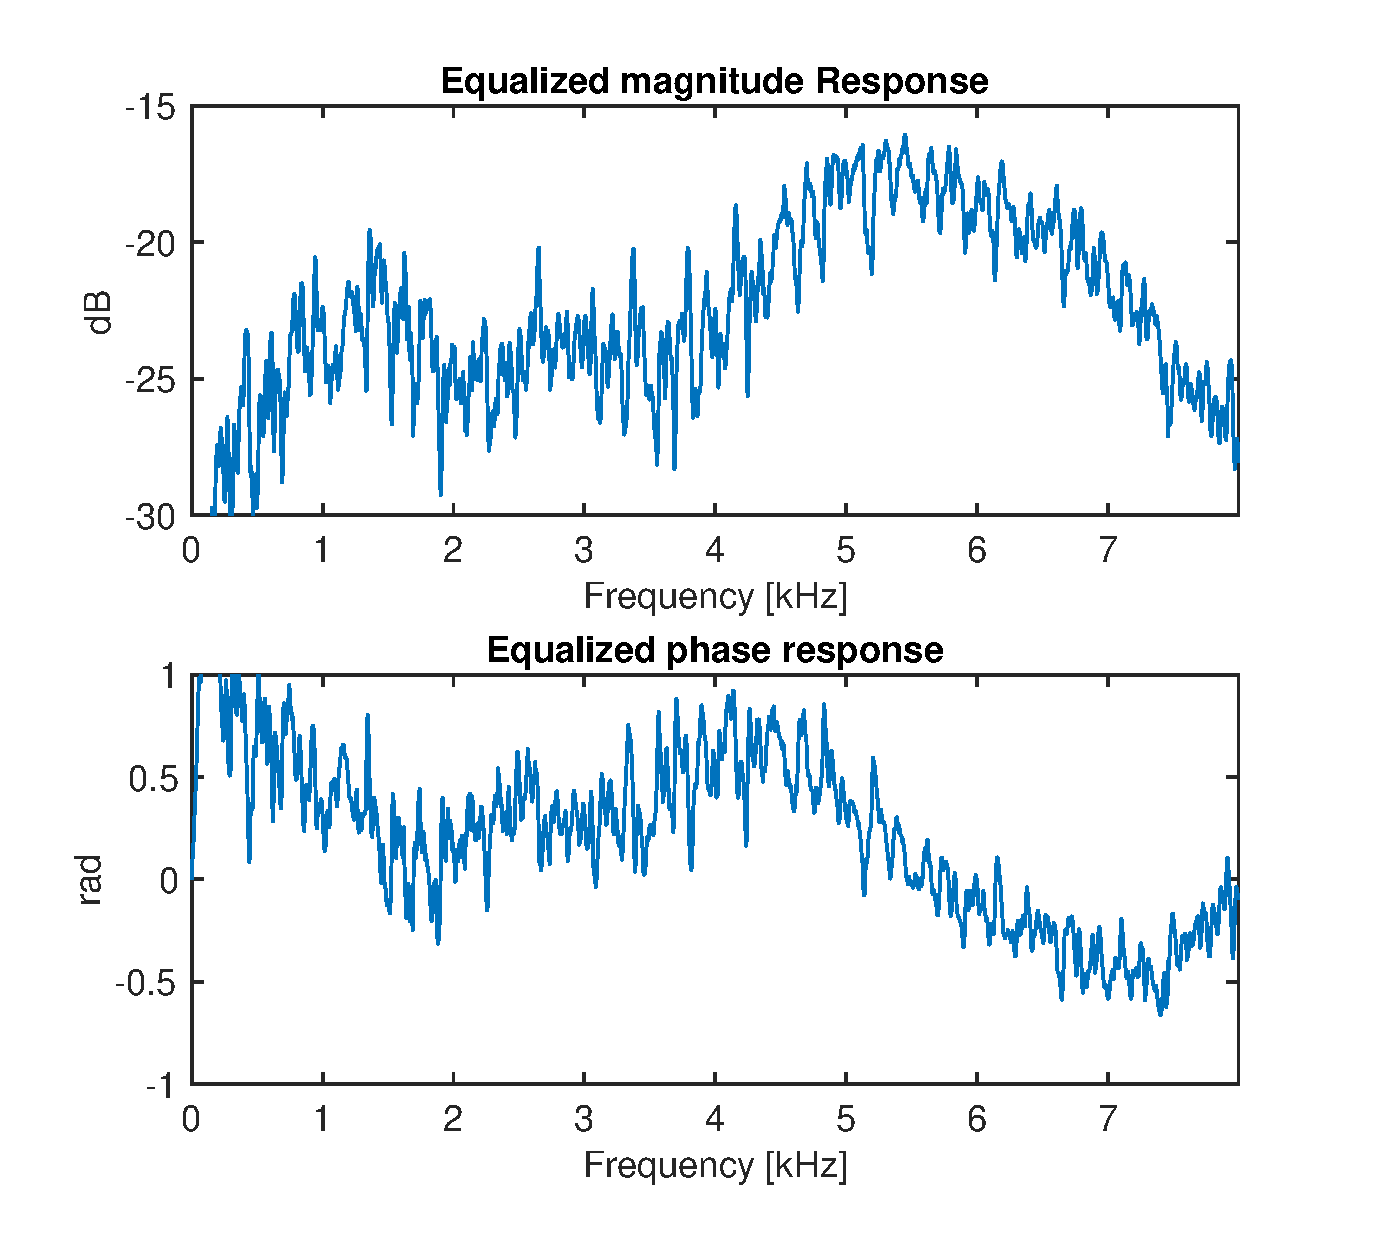
\includegraphics[width=\textwidth]{Equalized_RTF_SourceLength_4_Blind}
	\end{subfigure}
	\begin{subfigure}[b]{0.3\textwidth}
		\centering
		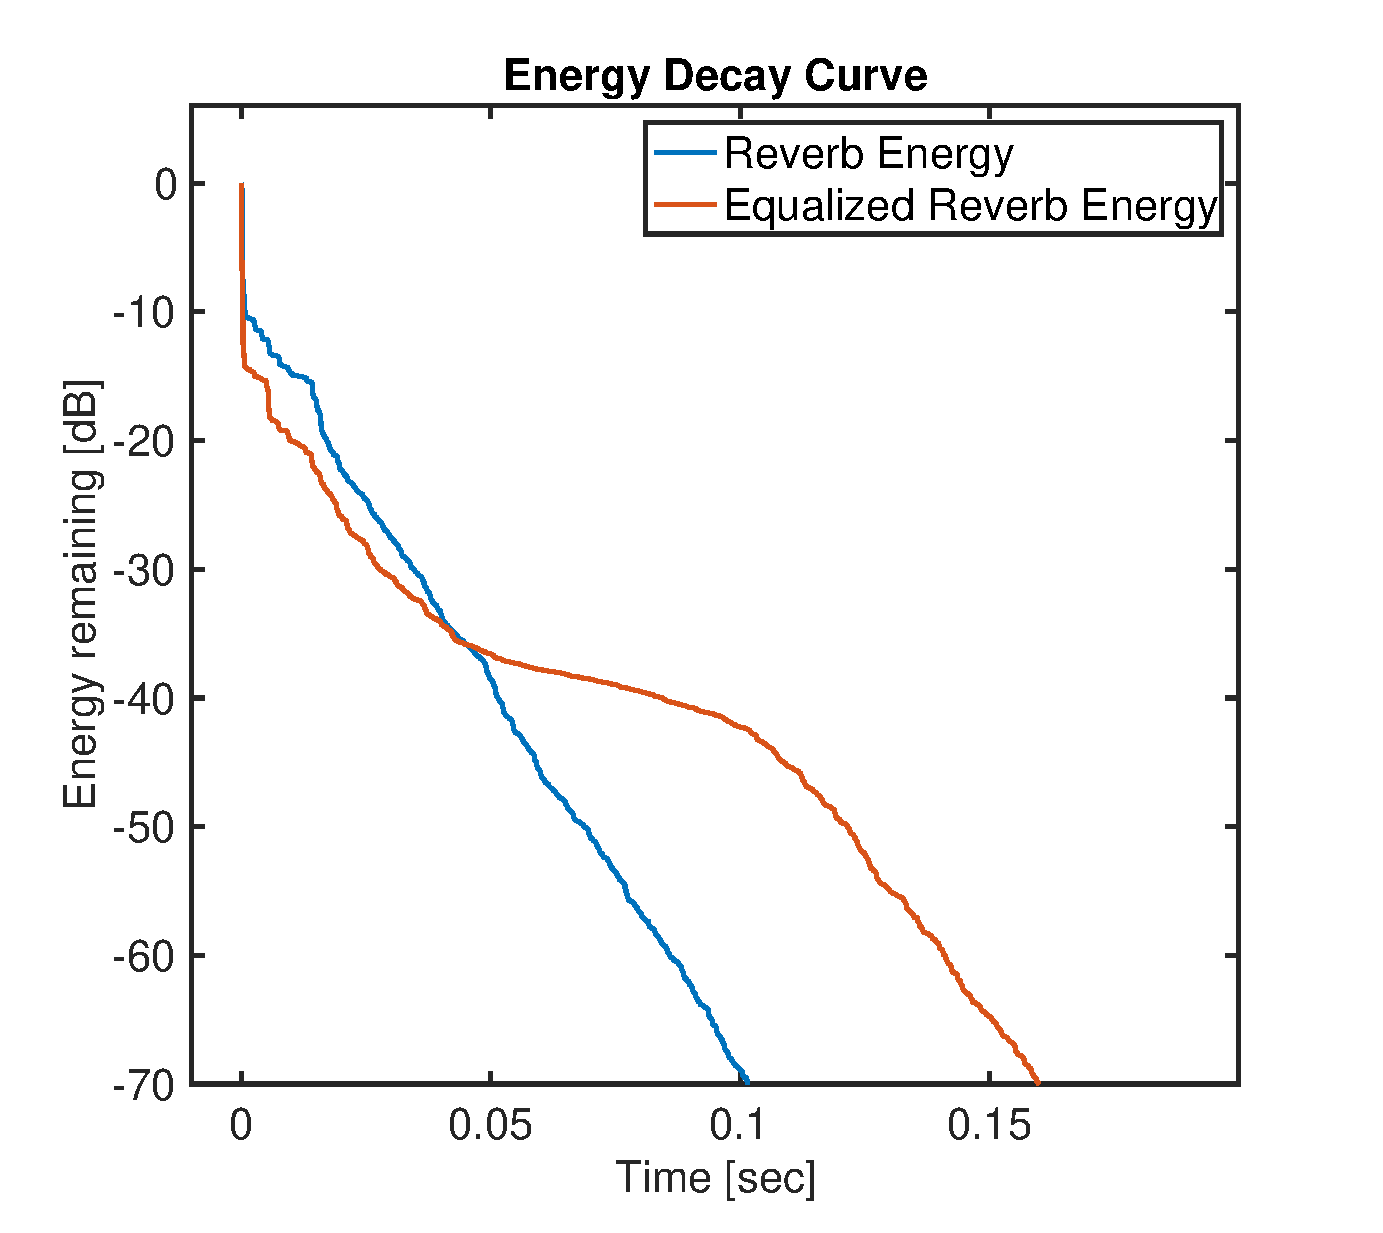
\includegraphics[width=\textwidth]{EDC_SourceLength_4_Blind}
	\end{subfigure}
	\caption{Delay-and-Predict dereverberation performance with the same speech sample (SA1.WAV, 58061 samples) looped to various data lengths to preserve the same spectrum. Source whitening prediction order was $\mathrm{p1} = 2 \cdot \mathrm{p2} \cdot (M-1)$ and multichannel linear prediction order was $\mathrm{p2} = \mathrm{N60} / (M-1)$. Source Whitening stage was performed on revererbant speech (i.e., blind).}
	\label{fig:params_source_length_compare}
\end{figure}

\textbf{TODO: Generate missing figures above, also add detailed ones to appendix, I think we can remove all the non blind ones from appendix}


...EDC Performance saturates around -35 dB beyond 3 loops.


This shows the dependency of LP performance on data length (reduces correlation variance).

Conclusion:
•	Performance depends on data length regardless of spectrum
•	Note: In LPC work I’ve done in the past, I got good performance for very short sequences (single phonemes), but this is for a very low-order LPC (order of 8-16 poles) --  a couple thoughts / explanations about this:
a.	Higher order LPC requires a lot of data is needed to analyze the fine time frequency characteristics (in low order, coarse resolution is sufficient to observe the location of a couple poles)?
b.	Higher order LPC requires a lot of data to estimate autocorrelation function out to very long lags?
c.	White noise filtered by a single pole (very low spectrum complexity) performs slightly better at low frequencies suggesting  (a) may be partially true
d.	As a final test, pre-computed and saved the whitened speech signal using very long sequence, but then extracted one 1:58061 iteration, and reran on just that. No improvement in performance compared to running on Signal Length = 58061 of non-whitened speech (SA1.wav). Reinforces that the source whitening dependency on data length exists regardless of speech spectrum.
*Note: Suprising that the whitened spectrum is identical for the two cases


\subsection{Source Spectrum}

Test: Same length different spectrum
•	Source whitening done on clean speech (no blind estimation)
•	Test: Speech is different length white noise sequences looped to length = 60 sec = 960000 (as original sequence length goes down, peakiness of spectrum goes up but final length doesn’t change)
•	RIR = SAL truncated to 100 msec = 1600 samples, M = 4 mics
•	P1 = 2 * p2 * (M-1)
•	P2 = N60 / (M-1)

\textbf{Source Spectrum Compare, Initial White noise sequence length = [0.1 sec 1 sec  10 sec], Blind}

\begin{figure}[H]
	\centering
	\begin{subfigure}[b]{0.3\textwidth}
		\centering
		\includegraphics[width=\textwidth]{S1_SourceSpectrum_100msecWhiteNoise_Blind}
	\end{subfigure}
	\begin{subfigure}[b]{0.3\textwidth}
		\centering
		\includegraphics[width=\textwidth]{Equalized_RTF_SourceSpectrum_100msecWhiteNoise_Blind}
	\end{subfigure}
	\begin{subfigure}[b]{0.3\textwidth}
		\centering
		\includegraphics[width=\textwidth]{EDC_SourceSpectrum_100msecWhiteNoise_Blind}
	\end{subfigure}
	\begin{subfigure}[b]{0.3\textwidth}
		\centering
		\includegraphics[width=\textwidth]{S1_SourceSpectrum_1secWhiteNoise_Blind}
	\end{subfigure}
	\begin{subfigure}[b]{0.3\textwidth}
		\centering
		\includegraphics[width=\textwidth]{Equalized_RTF_SourceSpectrum_1secWhiteNoise_Blind}
	\end{subfigure}
	\begin{subfigure}[b]{0.3\textwidth}
		\centering
		\includegraphics[width=\textwidth]{EDC_SourceSpectrum_1secWhiteNoise_Blind}
	\end{subfigure}
	\begin{subfigure}[b]{0.3\textwidth}
		\centering
		\includegraphics[width=\textwidth]{S1_SourceSpectrum_10secWhiteNoise_Blind}
	\end{subfigure}
	\begin{subfigure}[b]{0.3\textwidth}
		\centering
		\includegraphics[width=\textwidth]{Equalized_RTF_SourceSpectrum_10secWhiteNoise_Blind}
	\end{subfigure}
	\begin{subfigure}[b]{0.3\textwidth}
		\centering
		\includegraphics[width=\textwidth]{EDC_SourceSpectrum_10secWhiteNoise_Blind}
	\end{subfigure}
	\caption{Delay-and-Predict dereverberation performance with the source signal generated by looping various length white noise sequences looped the same data length (i.e., same data length, different spectra). Source whitening prediction order was $\mathrm{p1} = 2 \cdot \mathrm{p2} \cdot (M-1)$ and multichannel linear prediction order was $\mathrm{p2} = \mathrm{N60} / (M-1)$. Source Whitening stage was performed on revererbant speech (i.e., blind).}
	\label{fig:params_source_spectrum_compare}
\end{figure}

\textbf{Source Spectrum Compare, Initial SHAPED White noise sequence length = [0.1 sec 1 sec  10 sec], Blind}

\begin{figure}[H]
	\centering
	\begin{subfigure}[b]{0.3\textwidth}
		\centering
		\includegraphics[width=\textwidth]{S1_SourceSpectrum_10secShapedNoise_filter1_Blind}
	\end{subfigure}
	\begin{subfigure}[b]{0.3\textwidth}
		\centering
		\includegraphics[width=\textwidth]{Equalized_RTF_SourceSpectrum_10secShapedNoise_filter1_Blind}
	\end{subfigure}
	\begin{subfigure}[b]{0.3\textwidth}
		\centering
		\includegraphics[width=\textwidth]{EDC_SourceSpectrum_10secShapedNoise_filter1_Blind}
	\end{subfigure}
	\begin{subfigure}[b]{0.3\textwidth}
		\centering
		\includegraphics[width=\textwidth]{S1_SourceSpectrum_10secShapedNoise_filter2_Blind}
	\end{subfigure}
	\begin{subfigure}[b]{0.3\textwidth}
		\centering
		\includegraphics[width=\textwidth]{Equalized_RTF_SourceSpectrum_10secShapedNoise_filter2_Blind}
	\end{subfigure}
	\begin{subfigure}[b]{0.3\textwidth}
		\centering
		\includegraphics[width=\textwidth]{EDC_SourceSpectrum_10secShapedNoise_filter2_Blind}
	\end{subfigure}
		\begin{subfigure}[b]{0.3\textwidth}
		\centering
		\includegraphics[width=\textwidth]{S1_SourceSpectrum_10secShapedNoise_filter3_Blind}
	\end{subfigure}
	\begin{subfigure}[b]{0.3\textwidth}
		\centering
		\includegraphics[width=\textwidth]{Equalized_RTF_SourceSpectrum_10secShapedNoise_filter3_Blind}
	\end{subfigure}
	\begin{subfigure}[b]{0.3\textwidth}
		\centering
		\includegraphics[width=\textwidth]{EDC_SourceSpectrum_10secShapedNoise_filter3_Blind}
	\end{subfigure}
	\caption{Delay-and-Predict dereverberation performance with the source signal generated by filtering \qty{60}{\milli\sec} of speech with filters of various peakiness. Source whitening prediction order was $\mathrm{p1} = 2 \cdot \mathrm{p2} \cdot (M-1)$ and multichannel linear prediction order was $\mathrm{p2} = \mathrm{N60} / (M-1)$. Source Whitening stage was performed on revererbant speech (i.e., blind).}
	\label{fig:params_source_spectrum_shaped_compare}
\end{figure}

Conclusion:
•	Spectrum has a huge impact on performance, independent of signal length
•	It seems more related to complexity of spectrum than to peakiness
a.	Peakiness and complexity increase – major impact


\section{Time Alignment of RIRs and Linear Combiner}

Test:
•	Synthetic RIRs, delayed manually (incremental delay added per channel), T60=100msec
•	L channel = N60 * 2 = 3200 samples (~120 dB attenuation)
•	Source = SA1.wav looped for 20 sec
•	S1 on clean speech
•	Figures saved (.fig)

\textbf{Incremental delay of 2 sample}

\begin{figure}[H]
	\includegraphics[width=0.99\textwidth]{MC_EIR_TimeAlignment_2sampleDelay}
	\centering
	\caption{Showing the impact of RIR time alignment on multichannel linear prediction performance. The RIRs (left column) were synthetically generated exponentially decaying gaussians and an incremental delay of 2 samples was added to each channel. The right column shows the result of each individual prediction error filter (i.e., the top-most one is the result of predicting the current sample of microphone 1 from the past samples of microphones 1-4)}
	\label{fig:params_MC_EIR_TimeAlignment_2sampleDelay}
\end{figure}

See discussion in notes.

Add discussion about linear combiner and why the weighting vector suggested by slock makes sense (all based on time alignment)

\begin{figure}[H]
	\centering
	\begin{subfigure}[b]{0.32\textwidth}
		\centering
		\includegraphics[width=\textwidth]{EIR_TimeAlignment_2sampleDelay}
	\end{subfigure}
	\hfill
	\begin{subfigure}[b]{0.32\textwidth}
		\centering
		\includegraphics[width=\textwidth]{Equalized_RTF_TimeAlignment_2sampleDelay}
	\end{subfigure}
	\hfill
	\begin{subfigure}[b]{0.32\textwidth}
		\centering
		\includegraphics[width=\textwidth]{EDC_TimeAlignment_2sampleDelay}
	\end{subfigure}
	\hfill
	\caption{Delay-and-Predict dereverberation performance an incremental 2-sample delay added to each channel.}
	\label{fig:params_TimeAlignment_2sampleDelay}
\end{figure}


\textbf{No Delay}

\begin{figure}[H]
	\includegraphics[width=0.99\textwidth]{MC_EIR_TimeAlignment_0sampleDelay}
	\centering
	\caption{Repeating with no time delay}
	\label{fig:params_MC_EIR_TimeAlignment_0sampleDelay}
\end{figure}

\begin{figure}[H]
	\centering
	\begin{subfigure}[b]{0.32\textwidth}
		\centering
		\includegraphics[width=\textwidth]{EIR_TimeAlignment_0sampleDelay}
	\end{subfigure}
	\hfill
	\begin{subfigure}[b]{0.32\textwidth}
		\centering
		\includegraphics[width=\textwidth]{Equalized_RTF_TimeAlignment_0sampleDelay}
	\end{subfigure}
	\hfill
	\begin{subfigure}[b]{0.32\textwidth}
		\centering
		\includegraphics[width=\textwidth]{EDC_TimeAlignment_0sampleDelay}
	\end{subfigure}
	\hfill
	\caption{Delay-and-Predict dereverberation performance for perfectly time-aligned RIRs}
	\label{fig:params_TimeAlignment_0sampleDelay}
\end{figure}

\section{Algorithmic Complexity Analysis}

\begin{figure}[H]
	\centering
	\begin{subfigure}[b]{0.45\textwidth}
		\centering
		\includegraphics[width=\textwidth]{complexity_ops_comparison}
	\end{subfigure}
	\hfill
	\begin{subfigure}[b]{0.45\textwidth}
		\centering
		\includegraphics[width=\textwidth]{complexity_ops_comparison_zoomed}
	\end{subfigure}
	\caption{Analysis of the computational complexities of Least Squares solution and Inverse filter implementations as a function of T60, For $M=4$ microphones, $\mathrm{p2} = \mathrm{N60}/(M-1)$ and $\mathrm{p1} = 1.25 \cdot \mathrm{p2} \cdot (M-1)$. Complexity of LMS Solution also shown for comparison.}
	\label{fig:complexity_operations}
\end{figure}

\begin{figure}[H]
	\centering
	\begin{subfigure}[b]{0.45\textwidth}
		\centering
		\includegraphics[width=\textwidth]{complexity_mem_comparison}
	\end{subfigure}
	\hfill
	\begin{subfigure}[b]{0.45\textwidth}
		\centering
		\includegraphics[width=\textwidth]{complexity_mem_comparison_zoomed}
	\end{subfigure}
	\caption{Analysis of the algorithmic memory requirements  of Least Squares solution (could be temporary memory) and Inverse filter implementations (persistent memory) as a function of T60, For M=4 microphones, $\mathrm{p2} = \mathrm{N60}/(M-1)$ and $\mathrm{p1} = 1.25 \cdot \mathrm{p2} \cdot (M-1)$. Memory requirements of LMS Solution also shown for comparison.}
	\label{fig:complexity_memory}
\end{figure}



\section{Conclusions}

Summarize the role and requirements for each parameter



\section{Appendices}

\subsection{MC-LP Order}

\textbf{p2 = N60 / (M-1)  (MINT based on T60)}

\begin{figure}[H]
	\centering
	%\begin{subfigure}[b]{0.49\textwidth}
	%	\centering
	%	\includegraphics[width=\textwidth]{S1_N60_div_M_minus_1}
	%\end{subfigure}
	%\hfill
	\begin{subfigure}[b]{0.32\textwidth}
		\centering
		\includegraphics[width=\textwidth]{Equalized_RTF_N60_div_M_minus_1}
	\end{subfigure}
	\hfill
	\begin{subfigure}[b]{0.32\textwidth}
		\centering
		\includegraphics[width=\textwidth]{EIR_N60_div_M_minus_1}
	\end{subfigure}
	\hfill
	\begin{subfigure}[b]{0.32\textwidth}
		\centering
		\includegraphics[width=\textwidth]{EDC_N60_div_M_minus_1}
	\end{subfigure}
	\hfill
	\caption{Delay-and-Predict dereverberation performance with multichannel linear prediction order $\mathrm{p2} = \mathrm{N60} / (M-1)$, where N60 is the number of samples corresponding to the T60 and $M$ is the number of channels (i.e., the MINT condition based on T60 rather than the FIR RIR length). Figure \ref{fig:params_p2_stage1} shows the common source whitening filter used.}
	\label{fig:params_p2_N60}
\end{figure}

\textbf{p2 = 0p75 * N60 / (M-1) (Suboptimal)}

\begin{figure}[H]
	\centering
	%\begin{subfigure}[b]{0.49\textwidth}
	%	\centering
	%	\includegraphics[width=\textwidth]{S1_0p75N60_div_M_minus_1}
	%\end{subfigure}
	%\hfill
	\begin{subfigure}[b]{0.32\textwidth}
		\centering
		\includegraphics[width=\textwidth]{Equalized_RTF_0p75N60_div_M_minus_1}
	\end{subfigure}
	\hfill
	\begin{subfigure}[b]{0.32\textwidth}
		\centering
		\includegraphics[width=\textwidth]{EIR_0p75N60_div_M_minus_1}
	\end{subfigure}
	\hfill
	\begin{subfigure}[b]{0.32\textwidth}
		\centering
		\includegraphics[width=\textwidth]{EDC_0p75N60_div_M_minus_1}
	\end{subfigure}
	\hfill
	\caption{Delay-and-Predict dereverberation performance with multichannel linear prediction order $\mathrm{p2} = 0.75 \cdot \mathrm{N60} / (M-1)$, where N60 is the number of samples corresponding to the T60 and $M$ is the number of channels (i.e., suboptimal with respect to the MINT condition based on T60 rather than the FIR RIR length). Figure \ref{fig:params_p2_stage1} shows the common source whitening filter used.}
	\label{fig:params_p2_0p75_N60}
\end{figure}

\textbf{p2 = 0.5 * N60 / (M-1) (More suboptimal)}

\begin{figure}[H]
	\centering
	%\begin{subfigure}[b]{0.49\textwidth}
	%	\centering
	%	\includegraphics[width=\textwidth]{S1_0p5N60_div_M_minus_1}
	%\end{subfigure}
	%\hfill
	\begin{subfigure}[b]{0.32\textwidth}
		\centering
		\includegraphics[width=\textwidth]{Equalized_RTF_0p5N60_div_M_minus_1}
	\end{subfigure}
	\hfill
	\begin{subfigure}[b]{0.32\textwidth}
		\centering
		\includegraphics[width=\textwidth]{EIR_0p5N60_div_M_minus_1}
	\end{subfigure}
	\hfill
	\begin{subfigure}[b]{0.32\textwidth}
		\centering
		\includegraphics[width=\textwidth]{EDC_0p5N60_div_M_minus_1}
	\end{subfigure}
	\hfill
	\caption{Delay-and-Predict dereverberation performance with multichannel linear prediction order $\mathrm{p2} = 0.5 \cdot \mathrm{N60} / (M-1)$, where N60 is the number of samples corresponding to the T60 and $M$ is the number of channels (i.e., More suboptimal with respect to the MINT condition based on T60 rather than the FIR RIR length). Figure \ref{fig:params_p2_stage1} shows the common source whitening filter used.}
	\label{fig:params_p2_0p5_N60}
\end{figure}

\subsection{Source Whitening Order}

\textbf{p1 = 1000}

\begin{figure}[H]
	\centering
	\begin{subfigure}[b]{0.49\textwidth}
		\centering
		\includegraphics[width=\textwidth]{S1_p1_1000}
	\end{subfigure}
	\hfill
	\begin{subfigure}[b]{0.49\textwidth}
		\centering
		\includegraphics[width=\textwidth]{Equalized_RTF_p1_1000}
	\end{subfigure}
	\hfill
	\begin{subfigure}[b]{0.49\textwidth}
		\centering
		\includegraphics[width=\textwidth]{EIR_p1_1000}
	\end{subfigure}
	\hfill
	\begin{subfigure}[b]{0.49\textwidth}
		\centering
		\includegraphics[width=\textwidth]{EDC_p1_1000}
	\end{subfigure}
	\hfill
	\caption{Delay-and-Predict dereverberation performance with source whitening prediction order $\mathrm{p1} = 1000$ and multichannel linear prediction order $\mathrm{p2} = \mathrm{N60} / (M-1)$.}
	\label{fig:params_p1_1000}
\end{figure}

\textbf{p1 = p2 * (M-1) (whitened on the same spectral resolution as the MC-LP equalizer)}

\begin{figure}[H]
	\centering
	\begin{subfigure}[b]{0.49\textwidth}
		\centering
		\includegraphics[width=\textwidth]{S1_p1_based_on_p2}
	\end{subfigure}
	\hfill
	\begin{subfigure}[b]{0.49\textwidth}
		\centering
		\includegraphics[width=\textwidth]{Equalized_RTF_p1_based_on_p2}
	\end{subfigure}
	\hfill
	\begin{subfigure}[b]{0.49\textwidth}
		\centering
		\includegraphics[width=\textwidth]{EIR_p1_based_on_p2}
	\end{subfigure}
	\hfill
	\begin{subfigure}[b]{0.49\textwidth}
		\centering
		\includegraphics[width=\textwidth]{EDC_p1_based_on_p2}
	\end{subfigure}
	\hfill
	\caption{Delay-and-Predict dereverberation performance with source whitening prediction order $\mathrm{p1} = \mathrm{p2} \cdot (M-1)$ and multichannel linear prediction order $\mathrm{p2} = \mathrm{N60} / (M-1)$. I.e., The source whitening filter order is the same as the effective MINT filter order.}
	\label{fig:params_p1_based_on_p2}
\end{figure}

\textbf{p1 = 2 * p2  * (M-1) (Extra headroom)}

\begin{figure}[H]
	\centering
	\begin{subfigure}[b]{0.49\textwidth}
		\centering
		\includegraphics[width=\textwidth]{S1_p1_2x_p2}
	\end{subfigure}
	\hfill
	\begin{subfigure}[b]{0.49\textwidth}
		\centering
		\includegraphics[width=\textwidth]{Equalized_RTF_p1_2x_p2}
	\end{subfigure}
	\hfill
	\begin{subfigure}[b]{0.49\textwidth}
		\centering
		\includegraphics[width=\textwidth]{EIR_p1_2x_p2}
	\end{subfigure}
	\hfill
	\begin{subfigure}[b]{0.49\textwidth}
		\centering
		\includegraphics[width=\textwidth]{EDC_p1_2x_p2}
	\end{subfigure}
	\hfill
	\caption{Delay-and-Predict dereverberation performance with source whitening prediction order $\mathrm{p1} = 2 \cdot \mathrm{p2} \cdot (M-1)$ and multichannel linear prediction order $\mathrm{p2} = \mathrm{N60} / (M-1)$. I.e., The source whitening filter order is twice the effective MINT filter order.}
	\label{fig:params_p1_2x_p2}
\end{figure}

... beyond about p1 = 1.25 * p2 * (M-1) EDC performance saturates at approximately -35 dB reverb attenuation.

\subsection{Source Properties: Data Length}

\textbf{Signal Length = 58061 (num loops = 1)}

\begin{figure}[H]
	\centering
	\begin{subfigure}[b]{0.49\textwidth}
		\centering
		\includegraphics[width=\textwidth]{S1_SourceLength_1_NotBlind}
	\end{subfigure}
	\hfill
	\begin{subfigure}[b]{0.49\textwidth}
		\centering
		\includegraphics[width=\textwidth]{Equalized_RTF_SourceLength_1_NotBlind}
	\end{subfigure}
	\hfill
	\begin{subfigure}[b]{0.49\textwidth}
		\centering
		\includegraphics[width=\textwidth]{EIR_SourceLength_1_NotBlind}
	\end{subfigure}
	\hfill
	\begin{subfigure}[b]{0.49\textwidth}
		\centering
		\includegraphics[width=\textwidth]{EDC_SourceLength_1_NotBlind}
	\end{subfigure}
	\hfill
	\caption{Delay-and-Predict dereverberation performance for a \qty{3.6}{second} speech source (58061 samples). Source whitening prediction order was $\mathrm{p1} = 2 \cdot \mathrm{p2} \cdot (M-1)$ and multichannel linear prediction order was $\mathrm{p2} = \mathrm{N60} / (M-1)$. Source whitening filter was estimated using clean speech.}
	\label{fig:params_source_length_1_not_blind}
\end{figure}

\begin{figure}[H]
	\centering
	\begin{subfigure}[b]{0.49\textwidth}
		\centering
		\includegraphics[width=\textwidth]{S1_SourceLength_1_Blind}
	\end{subfigure}
	\hfill
	\begin{subfigure}[b]{0.49\textwidth}
		\centering
		\includegraphics[width=\textwidth]{Equalized_RTF_SourceLength_1_Blind}
	\end{subfigure}
	\hfill
	\begin{subfigure}[b]{0.49\textwidth}
		\centering
		\includegraphics[width=\textwidth]{EIR_SourceLength_1_Blind}
	\end{subfigure}
	\hfill
	\begin{subfigure}[b]{0.49\textwidth}
		\centering
		\includegraphics[width=\textwidth]{EDC_SourceLength_1_Blind}
	\end{subfigure}
	\hfill
	\caption{Delay-and-Predict dereverberation performance for a  \qty{3.6}{second} speech source (58061 samples). Source whitening prediction order was $\mathrm{p1} = 2 \cdot \mathrm{p2} \cdot (M-1)$ and multichannel linear prediction order was $\mathrm{p2} = \mathrm{N60} / (M-1)$. Source whitening filter was estimated using reverberant speech (blind estimation).}
	\label{fig:params_source_length_1_blind}
\end{figure}



\textbf{Signal Length = 174183 (num loops = 3)}

\begin{figure}[H]
	\centering
	\begin{subfigure}[b]{0.49\textwidth}
		\centering
		\includegraphics[width=\textwidth]{S1_SourceLength_3_NotBlind}
	\end{subfigure}
	\hfill
	\begin{subfigure}[b]{0.49\textwidth}
		\centering
		\includegraphics[width=\textwidth]{Equalized_RTF_SourceLength_3_NotBlind}
	\end{subfigure}
	\hfill
	\begin{subfigure}[b]{0.49\textwidth}
		\centering
		\includegraphics[width=\textwidth]{EIR_SourceLength_3_NotBlind}
	\end{subfigure}
	\hfill
	\begin{subfigure}[b]{0.49\textwidth}
		\centering
		\includegraphics[width=\textwidth]{EDC_SourceLength_3_NotBlind}
	\end{subfigure}
	\hfill
	\caption{Delay-and-Predict dereverberation performance for a \qty{10.9}{second} speech source (174183 samples). The source was generated by looping the same \qty{3.6}{second} source 3 times to maintain the same spectrum. Source whitening prediction order was $\mathrm{p1} = 2 \cdot \mathrm{p2} \cdot (M-1)$ and multichannel linear prediction order was $\mathrm{p2} = \mathrm{N60} / (M-1)$. Source whitening filter was estimated using clean speech.}
	\label{fig:params_source_length_3_not_blind}
\end{figure}

\begin{figure}[H]
	\centering
	\begin{subfigure}[b]{0.49\textwidth}
		\centering
		\includegraphics[width=\textwidth]{S1_SourceLength_3_Blind}
	\end{subfigure}
	\hfill
	\begin{subfigure}[b]{0.49\textwidth}
		\centering
		\includegraphics[width=\textwidth]{Equalized_RTF_SourceLength_3_Blind}
	\end{subfigure}
	\hfill
	\begin{subfigure}[b]{0.49\textwidth}
		\centering
		\includegraphics[width=\textwidth]{EIR_SourceLength_3_Blind}
	\end{subfigure}
	\hfill
	\begin{subfigure}[b]{0.49\textwidth}
		\centering
		\includegraphics[width=\textwidth]{EDC_SourceLength_3_Blind}
	\end{subfigure}
	\hfill
	\caption{Delay-and-Predict dereverberation performance for a \qty{10.9}{second} speech source (174183 samples). The source was generated by looping the same \qty{3.6}{second} source 3 times to maintain the same spectrum. Source whitening prediction order was $\mathrm{p1} = 2 \cdot \mathrm{p2} \cdot (M-1)$ and multichannel linear prediction order was $\mathrm{p2} = \mathrm{N60} / (M-1)$. Source whitening filter was estimated using revererant speech (blind estimation).}
	\label{fig:params_source_length_3_blind}
\end{figure}

\subsection{Source Properties: Spectrum}

\textbf{Original length = 1 sec white noise, loop count = 60}

\begin{figure}[H]
	\centering
	\begin{subfigure}[b]{0.49\textwidth}
		\centering
		\includegraphics[width=\textwidth]{S1_SourceSpectrum_1secWhiteNoise_NotBlind}
	\end{subfigure}
	\hfill
	\begin{subfigure}[b]{0.49\textwidth}
		\centering
		\includegraphics[width=\textwidth]{Equalized_RTF_SourceSpectrum_1secWhiteNoise_NotBlind}
	\end{subfigure}
	\hfill
	\begin{subfigure}[b]{0.49\textwidth}
		\centering
		\includegraphics[width=\textwidth]{EIR_SourceSpectrum_1secWhiteNoise_NotBlind}
	\end{subfigure}
	\hfill
	\begin{subfigure}[b]{0.49\textwidth}
		\centering
		\includegraphics[width=\textwidth]{EDC_SourceSpectrum_1secWhiteNoise_NotBlind}
	\end{subfigure}
	\hfill
	\caption{Delay-and-Predict dereverberation performance with source being 1 second of white noise looped to 60 seconds. Source whitening prediction order was $\mathrm{p1} = 2 \cdot \mathrm{p2} \cdot (M-1)$ and multichannel linear prediction order was $\mathrm{p2} = \mathrm{N60} / (M-1)$. Source whitening filter was estimated using clean speech.}
	\label{fig:params_source_spectrum_1sec_not_blind}
\end{figure}

\begin{figure}[H]
	\centering
	\begin{subfigure}[b]{0.49\textwidth}
		\centering
		\includegraphics[width=\textwidth]{S1_SourceSpectrum_1secWhiteNoise_Blind}
	\end{subfigure}
	\hfill
	\begin{subfigure}[b]{0.49\textwidth}
		\centering
		\includegraphics[width=\textwidth]{Equalized_RTF_SourceSpectrum_1secWhiteNoise_Blind}
	\end{subfigure}
	\hfill
	\begin{subfigure}[b]{0.49\textwidth}
		\centering
		\includegraphics[width=\textwidth]{EIR_SourceSpectrum_1secWhiteNoise_Blind}
	\end{subfigure}
	\hfill
	\begin{subfigure}[b]{0.49\textwidth}
		\centering
		\includegraphics[width=\textwidth]{EDC_SourceSpectrum_1secWhiteNoise_Blind}
	\end{subfigure}
	\hfill
	\caption{Delay-and-Predict dereverberation performance with source being 1 second of white noise looped to 60 seconds. Source whitening prediction order was $\mathrm{p1} = 2 \cdot \mathrm{p2} * (M-1)$ and multichannel linear prediction order was $\mathrm{p2} = \mathrm{N60} / (M-1)$. Source whitening filter was estimated using revererant speech (blind estimation).}
	\label{fig:params_source_spectrum_1sec_blind}
\end{figure}


\textbf{Original length = 10 sec white noise, loop count = 6}

\begin{figure}[H]
	\centering
	\begin{subfigure}[b]{0.49\textwidth}
		\centering
		\includegraphics[width=\textwidth]{S1_SourceSpectrum_10secWhiteNoise_NotBlind}
	\end{subfigure}
	\hfill
	\begin{subfigure}[b]{0.49\textwidth}
		\centering
		\includegraphics[width=\textwidth]{Equalized_RTF_SourceSpectrum_10secWhiteNoise_NotBlind}
	\end{subfigure}
	\hfill
	\begin{subfigure}[b]{0.49\textwidth}
		\centering
		\includegraphics[width=\textwidth]{EIR_SourceSpectrum_10secWhiteNoise_NotBlind}
	\end{subfigure}
	\hfill
	\begin{subfigure}[b]{0.49\textwidth}
		\centering
		\includegraphics[width=\textwidth]{EDC_SourceSpectrum_10secWhiteNoise_NotBlind}
	\end{subfigure}
	\hfill
	\caption{Delay-and-Predict dereverberation performance with source being 10 seconds of white noise looped to 60 seconds (i.e., source is less peaky than the previous case). Source whitening prediction order was $\mathrm{p1} = 2 \cdot \mathrm{p2} * (M-1)$ and multichannel linear prediction order was $\mathrm{p2} = \mathrm{N60} / (M-1)$. Source whitening filter was estimated using clean speech.}
	\label{fig:params_source_spectrum_10sec_not_blind}
\end{figure}

\begin{figure}[H]
	\centering
	\begin{subfigure}[b]{0.49\textwidth}
		\centering
		\includegraphics[width=\textwidth]{S1_SourceSpectrum_10secWhiteNoise_Blind}
	\end{subfigure}
	\hfill
	\begin{subfigure}[b]{0.49\textwidth}
		\centering
		\includegraphics[width=\textwidth]{Equalized_RTF_SourceSpectrum_10secWhiteNoise_Blind}
	\end{subfigure}
	\hfill
	\begin{subfigure}[b]{0.49\textwidth}
		\centering
		\includegraphics[width=\textwidth]{EIR_SourceSpectrum_10secWhiteNoise_Blind}
	\end{subfigure}
	\hfill
	\begin{subfigure}[b]{0.49\textwidth}
		\centering
		\includegraphics[width=\textwidth]{EDC_SourceSpectrum_10secWhiteNoise_Blind}
	\end{subfigure}
	\hfill
	\caption{Delay-and-Predict dereverberation performance with source being 10 seconds of white noise looped to 60 seconds (i.e., source is less peaky than the previous case). Source whitening prediction order was $\mathrm{p1} = 2 \cdot \mathrm{p2} \cdot (M-1)$ and multichannel linear prediction order was $\mathrm{p2} = \mathrm{N60} / (M-1)$. Source whitening filter was estimated using revererant speech (blind estimation).}
	\label{fig:params_source_spectrum_10sec_blind}
\end{figure}


